\documentclass[]{usiinfthesis}
\usepackage{lipsum}
\usepackage[draft]{fixme}
\usepackage{tikz}
\usepackage{algorithm}
\usepackage[noend]{algpseudocode}
\usetikzlibrary{automata}
% \usepackage{adjustbox}
%\setstretch{1.05}

\usepackage{graphicx}
\usepackage{subfigure}
\usepackage{listings}
\usepackage{multirow}
\usepackage{amsmath}

\newcommand{\aseeker}{{AccelSeeker}} 
\newcommand{\eseeker}{{EnergySeeker}} 
\newcommand{\rseeker}{{RegionSeeker}} 
\newcommand{\multi}{MuLTiVersioning}
\newcommand{\simulator}{\texttt{gem5-aladdin}} 
\newcommand{\HW}{{Hardware}}
\newcommand{\SW}{{Software}}
\newcommand{\HLS}{{High Level Synthesis}}
\newcommand{\SoC}{{System-on-Chip}}
\newcommand{\htsf}{{H.264}}
\newcommand{\SoTA}{{state-of-the-art}}
\newcommand{\plm}{{private local memory}}
\newcommand{\plms}{{private local memories}}

\newcommand{\ML}{{Machine Learning}}
\newcommand{\RF}{{Random Forest}}
\newcommand{\SVM}{{Support Vector Machines}}
\newcommand{\NN}{{Near Neighbor}}
\newcommand{\ItRef}{{Iterative Refinement}}

\newcommand{\dataflow}{data flow}
\newcommand{\controlflow}{control flow}
\newcommand{\CFG}{Control Flow Graph}
\newcommand{\CFGs}{Control Flow Graphs}

\newcommand{\compute}{\texttt{compute bound}} 
\newcommand{\iobound}{\texttt{I/O bound}} 

%algorithms
\newcommand{\exact}{\texttt{exact}}
\newcommand{\greedy}{\texttt{greedy}}
\newcommand{\exactC}{\texttt{exact-on-cropped}}

\newcommand{\candidate}{{AccelCand}} 
\newcommand{\candidates}{{AccelCand}s} 
\newcommand{\candidateW}{candidate} 
\newcommand{\candidatesW}{candidates} 

% \newcommand{\htsf}{\texttt{h264}}
\newcommand{\adpcm}{\texttt{adpcm}}
\newcommand{\sha}{\texttt{sha}}
\newcommand{\jpeg}{\texttt{jpeg}}
\newcommand{\mpeg}{\texttt{mpeg2}}
\newcommand{\aes}{\texttt{aes}}
\newcommand{\dfmul}{\texttt{dfmul}}
\newcommand{\dfsin}{\texttt{dfsin}}
\newcommand{\gsm}{\texttt{gsm}}
\newcommand{\stencil}{\texttt{stencil}}

\newcommand{\rsprobname}{\emph{Region Selection}} 
\newcommand{\asprobname}{\emph{Accel Selection}} 

\newcommand{\numofhtsfregs}{1745} % number of regions for h264
\newcommand{\numofjpegregs}{168} %number of regions for jpeg
\newcommand{\numberOfcandidates}{{63}} 

%change 'sl' to 'bf' for bold, or 'normalfont' for no special
%formatting
\captionsetup{labelfont={sl,sf}}

\lstdefinelanguage{algebra}
{morekeywords={import,sort,constructors,observers,transformers,axioms,if,
else,end},
sensitive=false,
morecomment=[l]{//s},
}


\title{Software Analysis for\\ Heterogeneous Computing Architectures} %compulsory
\subtitle{A research automation framework 
towards more efficient\\ HW/SW co-design} %optional 
\author{Georgios Zacharopoulos} %compulsory
\advisor{Professor Laura Pozzi} %compulsory
%\coadvisor{Co-Advisor} %optional
\Day{21} %compulsory
\Month{October} %compulsory
\Year{2019} %compulsory, put only the year
\place{Lugano} %compulsory
\programDirector{The PhD program Director \emph{pro tempore}} %compulsory


\committee{%
  \committeeMember{Alonzo Church}{University of California, Los Angeles, USA}
  \committeeMember{Alan M. Turing}{Princeton University, USA}
  %there can as many members as you like
} %the committee is compulsory

\dedication{To my parents Areti and Dimitris.\\For always being there for me.} %optional
\openepigraph{Legacy. What is a legacy?\\ Planting seeds in a garden you never get to see.}{Alexander Hamilton}
\openepigraph
{Men give me credit for some genius. All the genius I have lies in this; when I have a subject in hand, I study 
it profoundly. Day and night it is before me. My mind becomes pervaded with it. Then the effort that I have made 
is what people are pleased to call the fruit of genius. It is the fruit of labor and thought.} {Alexander Hamilton} %optional

\makeindex %optional, also comment out \theindex at the end

\begin{document}

\maketitle %generates the titlepage, this is FIXED

\frontmatter %generates the frontmatter, this is FIXED

\begin{abstract}
\textbf{NOTE: The abstract will be written in the end of the thesis.}\\
Performance increase, in terms of faster execution and higher energy efficiency, 
is a never-ending research endeavor  %story 
and does not come for free.
The breakdown of Dennard scaling, along with the seemingly inevitable end of 
Moore's law economic aspect, present a new challenge to computer architects striving to achieve
better performance in the modern computer systems. Heterogeneous computing is 
emerging as one of the solutions to overcome these limitations in order to keep the performance 
trend rising. This is achieved by turning the focus to specialized Hardware (HW) that 
can accelerate the execution of a Software (SW) application or a part of that application.
The goal is to design efficient HW/SW computer architectures, where a general purpose CPU
is coupled with a number of specialized HW accelerators.\\
The choice of which parts of an application to be accelerated, though, as well as the type 
of accelerators to be used, while taking into account the underlying memory system, are all
non-trivial research questions and depend heavily on the SW applications characteristics that
are going to be accelerated. Therefore, an in-depth SW analysis can be crucial, prior to 
designing a heterogeneous system, as it can provide valuable information and subsequently 
highly benefit performance. My initial research is revolving around various ways that SW
analysis, by extending the compiler frameworks and, hence, their potential, can offer this 
type of information and move one step closer towards optimizing and automating the design of 
hybrid HW/SW systems.
\end{abstract}

% \begin{abstract}[Zusammenfassung]
% optional, use only if  external advisor requires it in his/er
% language 
% \\

% \lipsum
% \end{abstract}

\begin{acknowledgements}
This is where I acknowledge people.

% \lipsum 
\end{acknowledgements}

\tableofcontents 
%\listoffigures %optional
% \listoftables %optional

\mainmatter

%
%
%  
%     INTRO
%
%
%

\chapter*{Introduction}
\addcontentsline{toc}{chapter}{Introduction}

Performance increase, in terms of faster execution and higher energy efficiency, 
is a never-ending research domain and does not come for free.
Living in an era where there is an immense amount of data, the demand for %the execution
performance by modern computing systems rises even more.
Technological giants, such as Google and Facebook, gather and compute loads of data, for instance 
during Machine Learning related applications and lengthy simulations. This large amount of data
processing requires immense computational power and ends up in lengthier and lengthier execution
 time.\par

Moore's law \cite{schaller1997moore}, an observation made by the co-founder of Intel Gordon Moore, 
predicts that the number of transistors that can be used in the same area of an integrated 
circuit will double roughly every 18 months. Complimentary to that, Dennard scaling 
\cite{dennard1974design}, 
also known as MOSFET scaling, states that voltage and current are 
proportional to the size of a transistor. Therefore, as long as the same chip area is retained, 
power stays constant and, at the same time, more transistors of smaller size can fit onto it.
Unfortunately, this is no longer the case. The transistor size has decreased over 
the years, but the amount of power per transistor has, recently, stopped decreasing accordingly,  
resulting in current leakage, a phenomenon also known as the 
Breakdown of Dennard scaling \cite{esmaeilzadeh2011dark}.\par

The breakdown of Dennard scaling \cite{esmaeilzadeh2011dark}, along with the seemingly inevitable 
end of Moore's law economic aspect \cite{simonite2016moore}, present a new challenge to computer 
architects striving to achieve
better performance in the modern computer systems.
Heterogeneous computing is emerging as one of the solutions in order to keep the performance 
trend rising. This is achieved by turning the focus to specialized Hardware (HW) that 
can accelerate the execution of a Software (SW) application or a part of that application. Specialized HW 
accelerators are implemented in platforms where they can be either reprogrammable, 
thus allowing for a large degree of flexibility as various implementations may take place utilizing
the HW resources of the platform (e.g. an FPGA board), or hardwired, such as an Application-Specific Integrated 
Circuit (ASIC). The first type of HW implementation sacrifices part of the potential 
performance achieved by allowing for flexible designs, as the same HW resources can be reprogrammed.
The latter offer no flexibility but can provide better performance in comparison to FPGAs. Under 
the scope of this research both HW implementations were considered.  \par
%
% This is a link
%
Since the performance of a general purpose CPU is becoming limited, due to physical and technological 
constrains, alternative computer architectures are required. Homogeneous parallel CPUs are used in 
order to expose parallelism of computation in SW applications, but performance is still restricted 
by the parts of computation that cannot be parallelized, a fact known also as Amdahl's law.
Instead of a 
general purpose CPU -- or homogeneous parallel CPUs -- managing the execution of SW applications, 
specialized pieces
of HW, namely accelerators, can be used alongside with a general purpose CPU and execute the
most demanding parts of an application in terms of computation. Consequently, the need for 
a powerful single CPU is no more that critical, as the execution can be offloaded to other
parts of HW as well. %The gain is twofold, as 
As a result, we achieve both a more balanced execution with 
the use of different HW resources, and we offload the execution of specific, more demanding 
parts of the computation to specialized HW accelerators.\par

One example of a widely spread heterogeneous architecture is the addition of a GPU to a CPU on the 
same chip, in order to exploit the parallelism and computing power that a GPU has to offer, when 
it comes to image processing and 3D graphics rendering. Other examples are general purpose CPUs 
coupled with dedicated HW that execute specific kernels or even full applications. The latter 
architecture could come in a number of variations, with one or more HW accelerators, and different 
types of coupling, tightly or loosely \cite{CotaJun15}. The design of the first option, tightly or 
co-processor model, is done by using the accelerator as an Instruction Set Extension in the default 
pipeline of the CPU. The latter implements the connection between CPU and accelerator loosely, without 
any knowledge of the underlying CPU micro-architecture.\par
%
% End of link
%
The goal of HW/SW co-design research is to design efficient heterogeneous computer architectures, so that the
time latency and energy requirements are ever decreasing. The heterogeneous system
that I considered during my research comprises a general purpose CPU, loosely coupled with a number of 
specialized HW accelerators, dedicated to the acceleration of specific parts of an application.\par

The choice of which parts of an application to be accelerated, though, as well as the type 
of accelerators to be used, while taking into account the underlying memory system, are all
non-trivial research questions and depend heavily on the SW applications characteristics that
are going to be accelerated. In addition to the accelerator selection problem, 
every HW accelerator can be synthesized with a number of optimizations embedded onto it, according to 
the characteristics of the task that is targeted for acceleration. For instance, in case 
a loop is included in the execution, there could be a loop unrolling factor taken into account during 
the synthesis of the accelerator that may dramatically affect execution time. Another example 
would be the addition of a memory buffer, e.g. a scratchpad memory, to reduce the memory latency
of the execution. Furthermore, the underlying memory system, as in every computer architecture, can
significantly affect the overall performance, due to communication latency, and should be taken into 
account during the selection of the accelerators to be implemented, along with their respective 
potential optimizations.\par

Therefore, an in-depth SW analysis can be crucial, prior to 
designing a heterogeneous system, as it can provide valuable information and subsequently 
highly benefit performance. Furthermore, such an analysis can be performed in short time (typically within a 
few seconds) and can be portable to other target applications or platforms. 
The research during my PhD has revolved around various ways that SW
analysis, by extending the LLVM compiler framework \cite{LattnerMar04} and, hence, its potential,
can guide a HW engineer %synthesizing HW accelerators 
by making informed decisions early in the development cycle.

\begin{figure}[t]
\centering
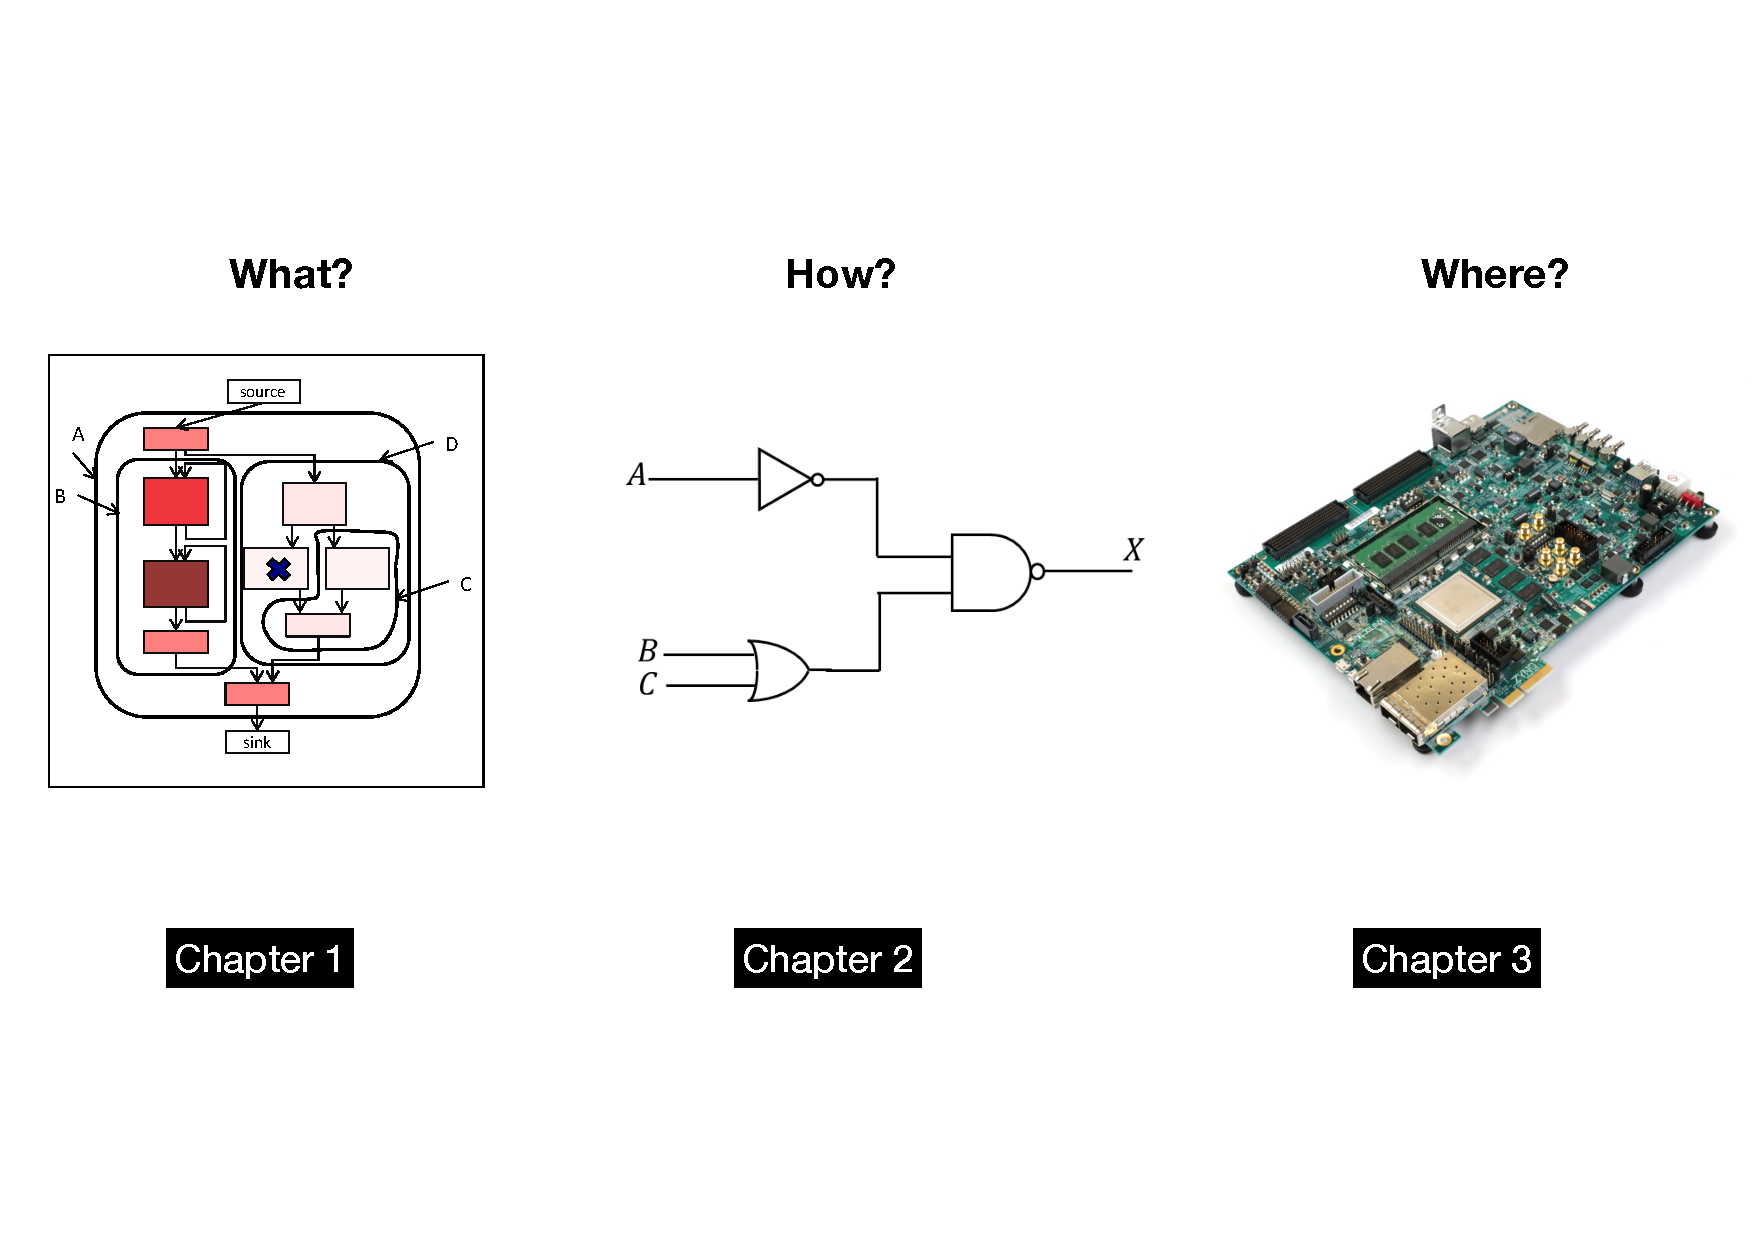
\includegraphics[width= 1 \linewidth]{figs/Research_Carol}
% a figure\dots
\caption{Overview of the research that has been conducted during my PhD and the respective chapters
of the PhD thesis.}
%\vspace{-0.5cm}
\label{fig:overview}
\end{figure}

An overview of the research conducted during my PhD is depicted in Figure \ref{fig:overview}.
This can be viewed as a map of this PhD thesis in order to navigate throughout my 
research time-line and present a high level view of how each piece is connected to each other.\par

Chapter 1 answers the question of {\em what} should be accelerated, namely which parts of 
computation, given a constraint on HW area resources. 
Under the scope of this chapter the \rseeker\ tool-chain is presented \cite{ZacharopoulosApr19}. 
\rseeker\ is an LLVM based framework 
that, given a SW application provided as input, identifies and selects, in a fully automatic fashion, HW 
accelerators under the constraint of an area (HW resources) budget. The granularity of the candidates for 
acceleration considered is that of a subgraph of the control flow graph of a function, with a single control 
input and a single control output. These candidates are called regions. After identification takes place, a 
selection algorithm solves the problem of 
finding the subset of the initial regions list that, under a given area constraint, maximizes the collective 
speedup obtained. The evaluation of \rseeker\ took place by using both an industrial tool, such as Xilinx
Vivado HLS \cite{VivadoHLSMar17}, and a research HW accelerator simulator, such as Aladdin \cite{ShaoJul14}. 
Experiments carried out with these tools revealed an improvement of performance compared to the \SoTA\
and a speedup gain of up to 4.6x. 
\par

In Chapter 2, the 
analysis that is presented attempts to answer the research question of {\em how} the identified and 
selected HW accelerators should be implemented in order to achieve improved performance. 
Under that scope, Data Reuse analysis, during the execution of a specific domain of applications, 
reveals the effectiveness of private local memory structures \cite{ZacharopoulosJan17}. 
This is achieved with the aid of compiler polyhedral analysis that detects the amount of data 
reuse on a specific domain of applications. The analysis provides automatically the appropriate dimensions 
of a memory buffer attached to the HW accelerator that would carry out the execution of the applications
and minimize the communication between the accelerator and the main memory.
Furthermore, for HW accelerators that contain loops, an optimal
Loop Unrolling factor can be predicted for each of the included loops \cite{ZacharopoulosJul18}. 
The most suitable Loop Unrolling factor
for each loop is defined according to the target of optimization, which can be either less use of HW
 resources or better speedup. With the aid of a prior LLVM based analysis 
 of the loops and Machine Learning classification, predictions can be performed on a set of loops and the respective 
Loop Unrolling factors may be subsequently applied during the synthesis phase of the accelerators. \par

Finally, Chapter 3 tackles the research question of what should be accelerated but at the same time
taking into account {\em where} the specialized HW is hosted.
An analysis of the system at hand and its memory hierarchy can affect vastly the selection
of HW accelerators and subsequently the performance achieved. Latency due to data exchange
between the HW accelerators and main memory could add a significant overhead to the overall 
computation time. In this chapter \aseeker, an LLVM based tool-chain, is presented. \aseeker\ 
performs thorough analysis of applications
and estimates memory latency along with computational latency of candidates for acceleration. The 
granularity of the candidates for acceleration is that of a subgraph of the entire call graph of 
the application. 
%with a root function (node) and zero outgoing edges of the identified subgraph. 
HW accelerators are selected by an algorithm that maximizes speedup, or energy efficiency 
under a given area budget. The evaluation 
of \aseeker\ took place on Zynq UltraScale platform by Xilinx, considering a demanding and complex 
application such as \htsf. With respect to methodologies based solely on profiling information \aseeker\ 
attained an improved performance with an up to 2x speedup over a general purpose SW processor.\\
Automating the design and implementation of heterogeneous systems, while
improving their performance is the broad goal of this PhD thesis. All chapters of this document 
attempt to provide a step closer on attaining this goal and expanding the \SoTA, as well as opening 
new paths to future work.

% \lipsum[1-4]

%
%
%
%
%  
%     CHAPTER 1
%
%
%
%
%

% \chapter[Short title]{A chapter title which will run over two lines --- it's for
%   testing purpose}
\chapter%[Automatic Identification and Selection of HW Accelerators]
{Automatic Identification and Selection of Accelerators}

Moving towards a heterogeneous era, HW accelerators, dedicated to a specific task, can
improve both speedup of execution and energy efficiency in comparison to a general 
purpose CPU or a set of homogeneous CPUs. 
Under the scope of the current chapter, the focus will be on HW accelerators that minimize
latency and increase speedup. Nonetheless, the identification and selection 
of which parts of the computation are to be implemented in HW is a complex and demanding task. 
A thorough understanding of the application to be accelerated is necessary, the HW resources
(area) budget is often tight and the granularity of the candidates for acceleration 
can dramatically affect the overall execution time. Furthermore, optimizations may be applied
to a given, identified HW accelerator and this can produce multiple versions of equivalent
computation instances, that in turn can result in various heterogeneous architectures with different
characteristics and different performance gains.
In order to address these issues I present an automated methodology
that receives as input the source code of a given application and outputs a number of 
HW accelerators to be considered for acceleration. Among these candidates a selection takes 
place that maximizes collective speedup, given an area constraint. Finally, 
multiple versions of the same candidate can be considered during the selection phase as well.

\section{Motivation}
\label{sec:mot}


\begin{figure}[t]
\centering
%\hspace*{-2cm}
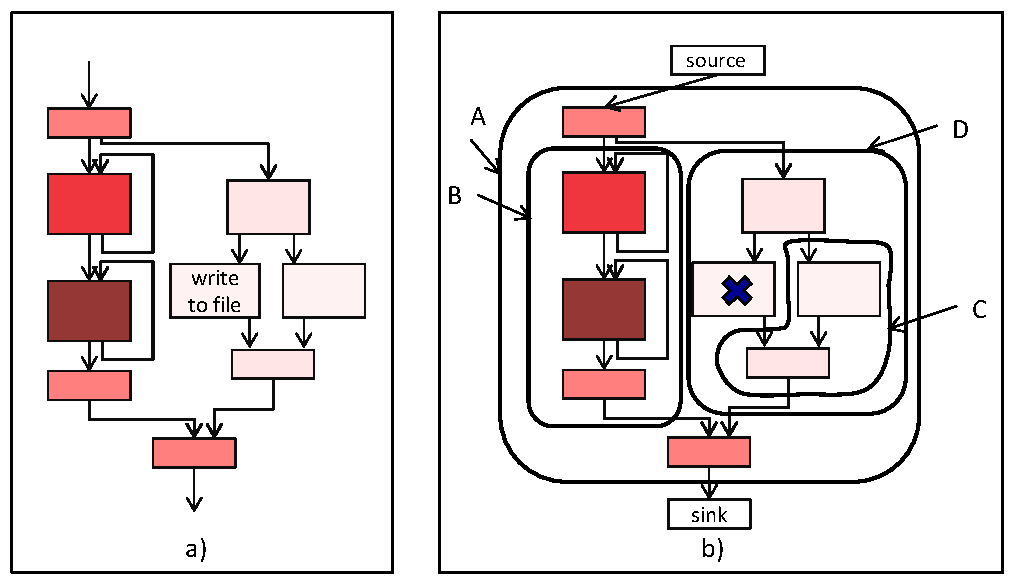
\includegraphics[width= .7 \linewidth]{Figs/cfg_example}
\caption{a) Example \CFG\ of a function, color-coded with frequency
  of execution (the darker the basic block, the more frequent). b) B
  and C are Valid Subgraphs; A and D are not Valid Subgraphs because
  they contain a forbidden node. B is also a CFG region, because it has a
  single \controlflow\ input and output.}
\label{fig:cfg-example}
\end{figure}


What is the rationale behind designer choices, when manually choosing
application parts to be accelerated in HW, and how can those choices
be replicated by an automated tool instead? Although it is possible,
perhaps, that \emph{all} of a designer's rationale cannot be
replicated automatically --- potentially because it requires a deep
knowledge of the application at hand --- it is certainly still
desirable to identify at least a subset of the actions that can be
automated.\par

Typically the designer aim will be: given an available accelerator
area, extract as much as possible of the computation, under the
constraint to require no more than that area, in order to maximize the
resulting speedup.\par 

Under the scope of this research I identify subgraphs of the \controlflow\ 
graph that have a single input control point and a single output control point, 
which herein will be called \emph{regions}, as good candidates for 
acceleration. The rationale
is that these subgraphs have a single entry point, and this
corresponds to the moment of execution when the accelerator is called,
and a single exit point, hence duly returning to a single location in
software when the accelerator is done. Note that this type of
\controlflow\ subgraph has been previously proposed and explored in
compiler research --- under the name of \emph{SESE} (Single Entry
Single Exit) in~\cite{AguilarJune16}, \cite{JohnsonJun94}, and under
the name of \emph{Simple Region} in an LLVM
implementation~\cite{LattnerMar04} --- with the aim of improving the
quality of \emph{SW code generation}, and as a scope for applying
compiler optimizations and parallelization. The idea of
identifying the same type of subgraph is borrowed and applied here in a 
novel way and to a different scenario and aim: that of automatically 
selecting HW accelerators.\par

A motivational example is provided in Figure~\ref{fig:cfg-example}a,
which depicts the CFG of an example function, color-coded with
frequency of execution (the darker the basic block, the more
frequent). A possible choice, when \emph{manually} identifying
accelerators, is to work at the granularity of functions: implement,
in HW, the function most frequently executed. However, this choice
might not be ideal, as the downside can be twofold: 1) a part of a
function might be less frequently executed than other parts (the right
side of the CFG, in the example in Figure~\ref{fig:cfg-example}a),
therefore effectively wasting accelerator real estate. 2) a part of a
function might contain non-synthesizable constructs --- such as the
``write to file" system call in Figure~\ref{fig:cfg-example}a or a function 
call that cannot be inlined.  On the
other side of the spectrum, choosing simply within the scope of single
basic blocks --- therefore, the body of the frequently executed loop
in the picture --- may not be ideal either, as the accelerator will be
called once in every iteration of the loop, which may results in a
large overhead. Furthermore, some speedup potential might be missed,
as larger CFG regions might expose better synthesis optimizations.\par

CFG regions are proposed therefore as candidates for
accelerators considering a granularity that can go from a
single loop to an entire function, and anything in between. 
The main body of my research for this work is the consideration 
of CFG regions as candidates and a method to 
automatically identify and select these regions.

%
%
% 1.2  Problem Formulation
%
%
%
%
%

\section{Problem Formulation}
\label{sec:prob}

The suggested methodology identifies and investigates the performance of regions
by analyzing, at the Intermediate Representation (IR) level, the
\CFGs\ of the functions comprising a target application. A CFG
represents the flow of control through a program.\par

Definition: \textbf{CFG}. A CFG is a Directed Cyclic Graph $G$, where
$V(G)$ is the set of nodes and $E(G)$ is the set of edges. Each node
in a CFG corresponds to a basic block in a function, and each edge to
the \controlflow\ within that function.\par

A source node is added, connected only to the entry basic block of
the function, and a sink node, connected only to the exit of the
function. Figure \ref{fig:cfg-example}b shows an example of CFG. A
node in the CFG is marked as forbidden if it corresponds to a basic
block containing instructions that cannot be synthesized in HW --- for
example operating system calls.\par

Definition: \textbf{Valid Subgraph.}  A Valid Subgraph is any subgraph
of the CFG that does not contain a forbidden node. In
Figure~\ref{fig:cfg-example}b: B, and C are Valid Subgraphs; A and D
are not Valid Subgraphs because they contain a forbidden node.\par

Definition: \textbf{Region.} A region $R$ of a CFG $G$ is a Valid
Subgraph such that there exists a \emph{single} edge going from a node
in $V(G)\setminus V(R)$ to a node in $V(R)$ and a \emph{single} edge
going from a node in $V(R)$ to a node in $V(G)\setminus V(R)$. In
Figure~\ref{fig:cfg-example}b: B is a region, while C is not.\par

Under the scope of this chapter, all and only regions are considered as
candidates for identification of accelerators.
Given a merit $M()$ and cost $C()$ function for each region 
we can formulate the problem of selecting accelerators as follows:

\textbf{Problem: Region Selection}

Let $\mathcal{R} = \{ R_1, R_2, \ldots, R_n \}$ be a set of regions,
with associated cost and merit functions $C$ and $M$.
For any subset $X\subseteq \{1,2,\ldots,n\}$ of regions,
we denote by $M(X) = \sum_{i\in X} M(R_i)$ the sum of the merits of
its regions, and we denote by $C(X) = \sum_{i\in X} C(R_i)$ the sum of
the costs of its regions.

We want to select a subset $X$ of regions such that
\begin{enumerate}
\item No two regions belonging to the same CFG overlap, i.e.,
  $V(R_i)\cap V(R_j) = \emptyset$, for all $1\le i,j\le n$
\item The cost $C(X)$ is within a user-given cost budget $C_{\max}$
\item The merit $M(X)$ is maximized
\end{enumerate}

This problem definition maps to what we have identified in the previous 
section as the designer aim: given an available
accelerator area, extract as much as possible of the computation,
under the constraint to require no more than that area, in order to
maximize the resulting speedup.

%
%
% 1.3  Selection Algos
%
%
%
%
%

\section{Region Selection Algorithms}
\label{sec:rs_algos}


The \rsprobname\ Problem requires a previously identified set of regions
as input. To identify regions, and hence gather such set, an existing LLVM 
pass is reused, which in turn is based on an algorithm of linear
time complexity published in~\cite{JohnsonJun94}. Then, given the
available set of regions, the more computationally expensive
\rsprobname\ Problem must be tackled, and algorithms to solve it are
explained in the following.\par

\begin{figure}
\centering
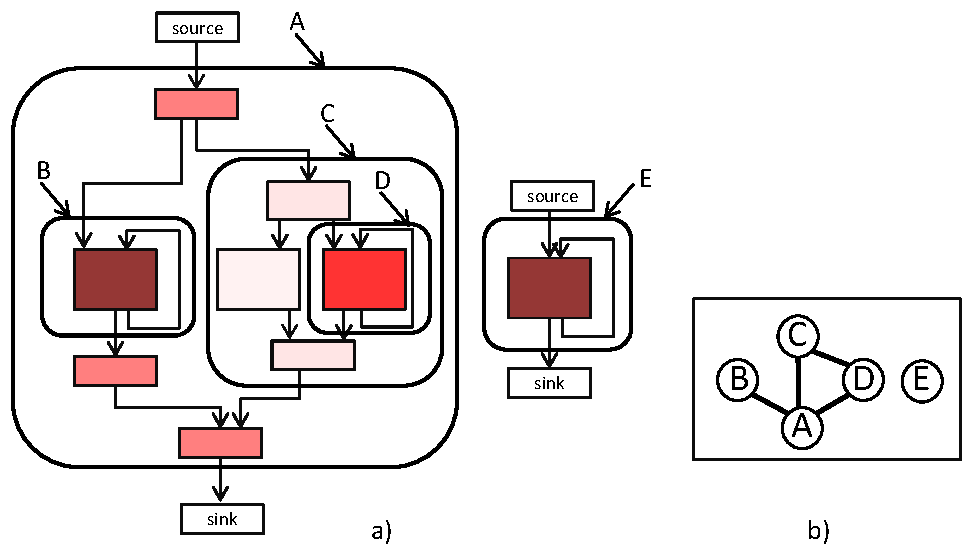
\includegraphics[width= .7 \linewidth]{figs/exact_example.pdf}
\caption{a) Running example, used to explain the selection algorithms:
  the CFGs of two functions are depicted, with five regions identified
  in them --- labelled from A to E. b) The overlap graph for the five
  regions.}
\label{fig:exact_example}
\end{figure}

Firstly an exponential, \exact\ branch-and-bound method
based on a binary-tree search is provided; secondly, a fast (polynomial)
non-exact, \greedy\ method; thirdly, a meet-in-the-middle approach,
still exponential but scaling faster than \exact, that we call
\exactC.\par

Before delving into the algorithm explanation, a running example
is provided in Figure~\ref{fig:exact_example}. The
Figure depicts the CFGs of two functions, and highlights five regions
identified within them (labeled A,B,C,D,E in the picture).\par
In the following, we denote by $O$ the set of region overlaps, i.e.,
the set
$$
\{ (i, j)\ |\ V(R_i)\cap V(R_j) \neq \emptyset \}\,.
$$
The edges of the graph represented in Figure ~\ref{fig:exact_example}b
correspond to the set $O$ of region overlaps, for the running example.


\subsection{Exact Method}
\label{sec:algo-exact}

In the \exact\ method the Problem \rsprobname\ is reduced to the
\emph{independent set problem}. In particular, we construct an
undirected graph $G$ where $V(G) = \{ 1, 2, \ldots, n \}$, i.e., there
is one node for each region, and $E(G) = O$, i.e., two nodes are
connected if the corresponding regions overlap. It is easy to see that
a set $\{ i_1, i_2, \ldots, i_r \}$ satisfies condition $1$ of the
\rsprobname\ Problem if it is an independent set of $G$.
Figure~\ref{fig:exact_example}b shows the overlap graph $G$
corresponding to the running example: region A overlaps with all
regions but E, hence edges are added linking A with B, C and D, and so
on. Examples of independent sets in this graph are $\{A\}$, $\{B,D\}$,
$\{B,C,E\}$.\par

The algorithm recursively explores the independent sets of $G$,
similarly to %the Bron-Kerbosch algorithm~
\cite{BronKerbosch73}, and
its steps will be followed with the aid of the running example, and
with its corresponding tree exploration, shown in
Figure~\ref{fig:exact_tree}. The algorithm maintains a set $X$, which
is the active independent set (initialized to $\emptyset$) and a set
$P$ of available nodes (initialized to $V(G)$). At each iteration, the
algorithm chooses a node $u$ in $P$ such that $C(X\cup \{u\})\le
C_{\max}$, i.e., it satisfies condition $2$ of the \rsprobname\ Problem,
and recursively explores the configurations
\begin{enumerate}
\item $X' = X\cup \{u\}$, $P' = P\setminus (\{u\}\cup N(u))$
\item $X' = X$, $P' = P\setminus \{u\}$
\end{enumerate}

where $N(u) = \{ v\ |\ (u,v)\in E(G) \}$ is the set of neighbours of
$u$ in the overlap graph.
Configuration 1 traverses all the independent sets that contain $X$
and $u$. The choice of $P'$ maintains this invariant, as all the
neighbours of $u$ are removed from $P$. Instead, configuration 2
traverses all the independent sets that contain $X$ but not $u$. Note
that any independent set is visited \emph{once only}.

This process can be exemplified through Figure~\ref{fig:exact_tree}:
the root of the tree represents the empty set, and set $P$ at this
point contains all regions. Then, inclusion of region A is first
explored, and the set P is updated by removing all regions overlapping
with A: $P = \{E\}$. According to the merit and costs of all regions
in this example, shown in the table within the picture, the merit (60)
and cost (35) of the solution currently explored is also updated.

At every point of the exploration, a new node $u$ is considered for
addition in the current independent set. If there is no node $u$
satisfying condition $2$ of the \rsprobname\ Problem, the algorithm
records the set $X$ and backtracks, as $X$ is maximal with respect to
condition $2$.  For the running example in
Figure~\ref{fig:exact_tree}, the cost budget $C_{\max}$ is equal to
$35$. Hence, exploration stops at $X=\{A\}$ because the cost budget
has been reached, and backtracks. The next region chosen is $B$, sets
$X$ and $P$ are again updated accordingly, to $X=\{B\}$ and
$P=\{C,D,E\}$, and exploration continues.

\emph{Optimization 1:} To speed up the search, the algorithm maintains
the maximum merit $M_{\max}$ of the independent sets explored so
far. In this way, if $M(X\cup P) < M_{\max}$ the algorithm can
backtrack, as no superset of $X$ has a merit larger than the maximum
one found so far. This optimization can be seen at work, among others,
in the tree-node where $X=\{B\}$ and $P=\{D,E\}$. In fact, $M_{\max}$
is $75$ at that point in the exploration (it was reached by set
$X=\{B,C,E\}$), while the current merit $M(\{B\})$ is $30$, and the
remaining potential gain of $P=\{D,E\}$ is $40$. $M_{\max}$ cannot be
reached, and the algorithm can backtrack.

\emph{Optimization 2:} To make the above exact pruning strategy
effective, the algorithm adopts the strategy of choosing the node $u$
with maximum merit among the ones which satisfy condition $2$ of the
\rsprobname\ Problem. In practice, this means that candidate regions are
considered in order of decreasing merit. In Subsection
\ref{subsec:algo-perf}, it is shown that these two optimizations greatly
increase the scalability of the exact method.

At the end of the exploration, the algorithm reports the set(s)
recorded with merit equal to $M_{\max}$, i.e., satisfying condition
$3$ of the \rsprobname\ Problem. In the running example, this
corresponds to set $X=\{B,C,E\}$.

\begin{figure*}[t]
\centering
%\includegraphics[width= \linewidth]{figs/figs_from_pptx/exact_tree.pdf}
\includegraphics[width= .9 \linewidth]{Figs/exact_tree.pdf}
\caption{Tree exploration performed by \exact, for the running example
  of Figure~\ref{fig:exact_example}, and for a cost budget of 35.}
\label{fig:exact_tree}
\end{figure*}


\subsection{Greedy Method}

The algorithm implementing a greedy selection maintains a set $X$
(initialized to $\emptyset$), which is the current partial solution,
and a set $P$ of available regions (initialized to $\{ 1, 2, \ldots, n
\}$). At each iteration, the algorithm selects the region $u$ in $P$
with largest merit such that $C(X\cup \{u\})\le C_{\max}$, and
continues to the next iteration with $X' = X\cup \{u\}$ and $P' =
P\setminus (\{u\}\cup\{ v\ |\ (u,v)\in O \})$. The choice of $P'$
guarantees that the set $X$ satisfies condition $1$ in each
iteration. If there is no region $u$ satisfying condition $2$ the
algorithm terminates and reports $X$.  In the running example of
Figure~\ref{fig:exact_tree}, this corresponds to simply stopping
exploration at set $X=\{A\}$.

Since the greedy method never backtracks, it is often trapped in local
minima, and therefore cannot guarantee optimality. On the other hand,
it converges to a solution very fast, and is used as a naive solution
for generating comparative results (Subsection \ref{subsec:algo-perf}).

\subsection{Exact-on-cropped Method}

The previous two algorithms represent two ends of the spectrum: exact
and exponential on one side; non-exact, fast and naive on the other.
A third solution, which strikes a balance between them, comes from the
observation that while the list of regions identified in an
application is long --- potentially too long to be processed exactly
--- the list of \emph{meaningful} regions is short, where by
meaningful is mean contributing tangibly to the overall speedup. In
other words, the distribution of regions with respect to speedup
provided is very skewed.

The third algorithm alternative is therefore to apply the \emph{exact}
algorithm (Section~\ref{sec:algo-exact}), but only to a \emph{cropped}
list of regions in input. This in practice corresponds to ignoring a
number of low-speedup regions in the selection problem. In
Subsection~\ref{subsec:algo-perf} it is showed that such approach, while of
course still of exponential complexity, can greatly improve the
scalability of the \exact\ algorithm, still retrieving high-quality
solutions.

\section{The RegionSeeker Framework}
\label{sec:rs}

The RegionSeeker framework is an automated methodology that 
identifies candidates for HW acceleration from application source 
code. An extensive SW analysis, based on the LLVM compiler infrastructure,
performs, apart from
the identification, an estimation of the performance gain (merit), along with
the HW resources (cost), of each candidate. Subsequently given a HW resources
constraint, a selection of the identified HW accelerators takes place that
maximizes the cumulative performance gain, as detailed in Section~\ref{sec:rs_algos}.
First the LLVM toolchain built for this purpose is analyzed, then the employed 
platform model and the benchmarks used for a comparative evaluation are detailed.

\subsection{LLVM Toolchain}

% LLVM RegionSeeker Analysis Pass.
% %
\begin{algorithm}[t]
\begin{flushleft}
\textbf{Input:}  Application written in C/C++\\
\textbf{Output:} List of Identified and Profiled Regions\\
\end{flushleft}
\begin{algorithmic}[1]
\Function{$RunOnFunction()$}{}
\State\Call{$Region\_List=NULL$}{}
\State\Call{$RI=getRegionInfoAnalysis()$}{}
  \For {$Region\ in\ Function$}
    \If {\Call{$RegionIsValid()$}{}}
      \State\Call{$EvaluateRegion$}{Region}
      \State{$Region\_List.Add(Region)$}     
    \EndIf
  \EndFor
  \State{$return\ Region\_List$}  

\EndFunction
\State
\State{$/* Estimate\ Merit\ for\ Region*/$}
\Function{$EvaluateRegion$}{Region}
  \For {$Basic\ Block\ in\ Region$}
    \State\Call{$getProfilingInfo$}{Basic\ Block}
  \EndFor
\EndFunction
\end{algorithmic}
\caption{LLVM Analysis Pass - Region Identification} 
\label{algo:reg}
\end{algorithm}

The analysis passes of \rseeker\ were built within the latest version (3.8) of the \emph{LLVM
  Compiler and Toolchain} \cite{LattnerMar04}. The LLVM infrastructure
provided the compiler ground in order to develop my own analysis
passes, as well as the tools used for profiling. 
\emph{Region Identification} pass, as depicted in Algorithm \ref{algo:reg}, 
was developed to identify and provide an initial estimated evaluation to 
the identified regions. The pass receives as input applications developed
in C or C++ and performs the analysis in the Intermediate Representation
(IR) level. \par

\emph{Region Identification} pass iterates over every function of the provided 
input applications and, using the existing \emph{RegionInfo} LLVM pass 
\cite{GrosserApr12}, identifies regions within every function. Subsequently, 
forbidden nodes within regions are identified and labeled, such as system
calls or calls to functions that are not inlined. The regions containing
these nodes are marked as invalid. Conversely, the valid regions are 
evaluated by a profiling via instrumentation routine.
Profiling via
instrumentation requires generating an instrumented version of the
code, which gives more detailed results than a sampling
profiler. Using this information, the basic blocks are annotated
 in each function with their respective execution frequency, along
 with the aid of \emph{ClrFreqCFGPrinter} LLVM pass \cite{ZacharopoulosMar17}.\par
 

By exploiting the execution frequency of every basic block, the respective evaluation 
for every region is computed, which is being associated to the region as estimated merit, 
and the region is being added to the list of identified regions.
The final output of our analysis pass is a list of valid regions, 
or else accelerator candidates, with an estimated merit attached to them.\par

The region list output is saved in a file, which is in turn processed by the 
selection algorithms \exact, \greedy\ and \exactC, which are 
implemented as standalone programs in C++.

\begin{figure}
\centering
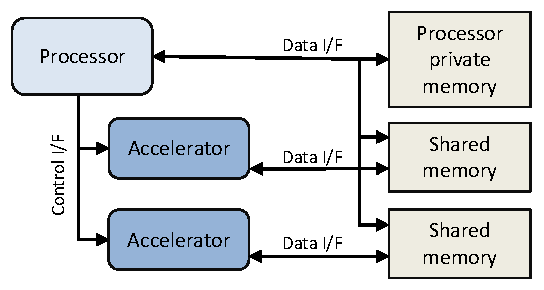
\includegraphics[width= .6 \linewidth]{figs/platform.pdf}
\caption{Target ASIP model, featuring a host processor interfacing
  special-function accelerators through control interfaces and shared
  data memories.}
\label{fig:platform}
\end{figure}

\subsection{Platform Model and Performance Metrics}
\label{subsec:platform}

The performance benefit achievable by application-specific
acceleration is dependent on multiple target-specific parameters,
including the adopted memory hierarchy, the employed bus protocol, the
interconnect strategy and the number of considered processors,
accelerators and memories.\par

In order to assess the performance of \rseeker, a system comprising
a single processor and multiple accelerators was assumed, exchanging shared data 
with scratchpad memories (Figure \ref{fig:platform}). 
The processor activates the accelerators via a memory-mapped
interface, thus requiring a transaction on the system bus. 
When activated, accelerators read and
write data to and from the scratchpads, computing their outputs, which
can then be accessed by the processor. In
this way, no data movement surrounding the execution of accelerations
is required. Accelerators are interfaced to scratchpad memories
with ports having a latency of one clock cycle. The
control interface between the processor and the accelerators has a
latency of 10 clock cycles.  These parameters correspond to the ones
employed by the \texttt{ap\_memory} and \texttt{s\_axilite}
interfaces, respectively, provided by Xilinx Vivado.\par

The run-times of the non-accelerated part of the considered
benchmarks are measured using the Gem5
simulator~\cite{BinkertFeb11}, modeling an ARMv8-A processor with an
issue width of 1. The processor model is atomic, with in-order
execution. It is interfaced with separate instruction and data
memories with an access latency of one clock cycle.\par

Hardware execution times are retrieved using \emph{two different HLS
  frameworks}: the Aladdin simulator and the Xilinx Vivado HLS
commercial tool-suite. Aladdin targets ASIC implementations. It
allows a fast evaluation, but does not produce a synthesizable netlist
as output; nonetheless, the estimations offered by this tool are
within 1\% of the ones derived from an RTL implementation
\cite{ShaoJul14}. Hardware instances generated with Vivado HLS are
instead intended for FPGA designs. Synthesis-runs within this
framework are more time-consuming, but provide exact cost (HW resources)
and merit (speedup) figures of each accelerator, as well as a direct
path to its realization.\par

The cost $C()$ of regions (and, for comparison, basic
blocks and functions) was computed as the amount of required resources. We
expressed them in terms of IC area in the case of Aladdin ($mM^2$), and the
maximum between their required flip-flops and look-up tables,
on a Virtex7 FPGA, in the case of Vivado. The merit $M()$ of a
region was set as the difference between its hardware and software run
time, across all its invocations in an application.

\subsection{Benchmarks}
\label{subsec:benchmarks}
\vspace{.3cm}


Real-world applications of varying size from the CHStone
embedded applications benchmark suite \cite{HaraMay08} were considered. 
\adpcm\ performs an encoding routine, whereas \sha\ is a secure hash
encryption algorithm, widely used for generating digital signatures
and the exchange of cryptographic keys. \aes\ is a symmetric-key
encryption algorithm. \gsm\ performs a linear predictive coding
analysis, used for mobile communication.  \dfmul\ and \dfsin\ are
smaller kernels that perform double-precision floating-point
multiplication and sine functions employing integer arithmetics.
\jpeg\ and \mpeg\ are larger applications, implementing JPEG and
MPEG-2 compression, respectively.  
% \subsection{Methodology}
% \label{subsec:meth}

% There are three parts comprising the methodology, detailed as follows.
% The first step is to automatically identify valid regions that are suitable candidates
% for HW acceleration. Secondly, an estimation of their potential merit, in terms of cycles saved
% (the difference between SW and HW execution cycles),
% is computed along with the respective cost, which is the HW resources (area) required
% for each region. Finally, a selection algorithm is utilized in order to optimally solve the 
% problem of selecting a subset of these
% regions that maximize the accumulated merit under a given cost, i.e., an area constraint.

% \subsubsection{Region Identification}
% \label{subsec:reg_id}

% To identify regions in both an automatic and efficient way, a
%  \emph{Region Identification} pass was developed under the version 3.8 
% of the \emph{LLVM Compiler framework} \cite{LattnerMar04}. 
% The pass receives as input applications developed in C or C++ and performs 
% their analysis at the Intermediate Representation (IR) level, a type
% of code used internally by LLVM to represent source code and allow
% data flow analysis and optimizations.\par

% The pass iterates over every function of an
%  application and, using the existing \emph{RegionInfo} LLVM pass 
% \cite{GrosserApr12}, identifies regions within every function.
% %, as seen in Figure \ref{fig:region}. 
% Subsequently, nodes that cannot be synthesized, such as system
% calls or calls to functions that are not inlined, are identified 
% and labeled as forbidden.
% %forbidden nodes inside regions are identified and labeled, such as system
% %calls or calls to functions that are not inlined. 
% The regions containing
% these nodes are marked as invalid. Conversely, the valid regions are 
% evaluated by a profiling-via-instrumentation routine.
% Profiling via
% instrumentation requires generating an instrumented version of the
% code, which gives more detailed results than a sampling
% profiler. 
% The output of the profiling is a file that contains information regarding 
% the execution frequency of each basic block and the total number of calls to each 
% function, i.e., the execution frequency of each function.
% Using this information, the basic blocks are annotated
%  in each function with their respective execution frequency. 
% % with the aid of \emph{ClrFreqCFGPrinter} LLVM pass \cite{ZacharopoulosMar17},
%  %that I have developed.


% % LLVM RegionSeeker Analysis Pass.
% % %
% \begin{algorithm}[t]
% \begin{flushleft}
% \textbf{Input:}  Application written in C/C++\\
% \textbf{Output:} List of Identified and Profiled Regions\\
% \end{flushleft}
% \begin{algorithmic}[1]
% \Function{$RunOnFunction()$}{}
% \State\Call{$Region\_List=NULL$}{}
% \State\Call{$RI=getRegionInfoAnalysis()$}{}
%   \For {$Region\ in\ Function$}
%     \If {\Call{$RegionIsValid()$}{}}
%       \State\Call{$EvaluateRegion$}{Region}
%       \State{$Region\_List.Add(Region)$}     
%     \EndIf
%   \EndFor
%   \State{$return\ Region\_List$}  
% \EndFunction

% \State
% \State{$/* Estimate\ Merit\ for\ Region*/$}
% \Function{$EvaluateRegion$}{Region}
%   \For {$Basic\ Block\ in\ Region$}
%     \State\Call{$getProfilingInfo$}{Basic\ Block}
%   \EndFor
% \EndFunction
% \end{algorithmic}
% \caption{LLVM Analysis Pass - Region Identification} 
% \label{algo:reg}
% \end{algorithm}

% \subsubsection{Merit and Cost Estimation}
% \label{subsec:mer_cost}

% The Region Identification pass, apart from the identification of regions detailed above, 
% performs an early evaluation of the merit and cost of a region, implemented
% directly within the LLVM tool-chain. The evaluation relies on the LLVM intermediate
% representation and does not need any manual modification to perform function out-lining
% on the benchmark source code. 
% The estimation of merit and the cost of a region is performed as follows.\par

% \emph{Merit Estimation.} 
% The merit of a region is defined as the total number of cycles saved in a HW accelerator 
% implementation compared to the respective SW implementation of the same piece of runtime 
% of a given application. Therefore the merit of a HW accelerator is estimated as the 
% difference between the \HW\ and \SW\ run time, across all its invocations in an application,
% taking into account the invocation overhead of calling a HW accelerator in a specific 
% heterogeneous architecture. The estimation of the HW run time is computed first in the 
% basic block (BB) level as the the critical path of the latency (in clock cycles) of the Data 
% Flow Graph (DFG) nodes. Runtime profiling information is used in order to determine the execution 
% frequency of each BB.
% Subsequently the delay of the entire region in HW is estimated by multiplying the critical path
% delay of each BB with the respective execution frequency and finally summing up the products, 
% according to the specific BBs that comprise the region.
% Software run-times are estimated in a similar fashion, but instead of computing critical paths 
% at the BB level, the sum of the latency (in clock cycles) of all its constituent operations is 
% computed, modeling that these are processed sequentially in software.\par

% \emph{Cost Estimation.} On the other side of the evaluation, the cost of a region 
% is estimated as the area (or HW resources) required to implement its DFG nodes. The area 
% is computed as the sum of look-up tables that is required for
% the DFG nodes of the respective HW accelerator. Each DFG node may take up a different amount
% of loop-up tables according to its complexity. The characterization for each DFG node was carried
% out with the aid of Vivado, a commercial \HLS\ tool, targeting a Virtex7 FPGA.\par
% % and its merit as the cycles saved between SW
% % and HW execution, where the latter is the delay of the nodes on the
% % DFG critical paths. Runtime profiling information is used in both SW and
% % HW latency estimations in order to determine the number of invocations for
% % each candidate.\par
% The final output of the analysis pass is a list of valid regions, 
% or else accelerator candidates, each annotated with an estimated merit and cost.
% The region list output is in turn processed by the 
% \exact\ selection algorithm implemented as standalone program in C++.
% % selection algorithms exact and greedy implemented as standalone programs in C++.


% \subsubsection{Region Selection Algorithm}
% \label{subsec:sel_algo}

% Given a merit $M()$ and cost $C()$ function for each region 
% we can formulate the problem of selecting accelerators as follows:\\
% \textbf{Problem: Region Selection}
% Let $\mathcal{R} = \{ R_1, R_2, \ldots, R_n \}$ be a set of regions,
% with associated cost and merit functions $C$ and $M$.
% For any subset $X\subseteq \{1,2,\ldots,n\}$ of regions,
% we denote by $M(X) = \sum_{i\in X} M(R_i)$ the sum of the merits of
% its regions, and we denote by $C(X) = \sum_{i\in X} C(R_i)$ the sum of
% the costs of its regions.

% We want to select a subset $X$ of regions such that
% \begin{enumerate}
% \item No two regions belonging to the same CFG overlap, i.e.,
%   $V(R_i)\cap V(R_j) = \emptyset$, for all $1\le i,j\le n$
% \item The cost $C(X)$ is within a user-given cost budget $C_{\max}$
% \item The merit $M(X)$ is maximized
% \end{enumerate}


% This problem definition maps to what we have identified in
% Section~\ref{sec:mot} as the designer aim: given an available
% accelerator area, extract as much as possible of the computation,
% under the constraint to require no more than that area, in order to
% maximize the resulting speedup.\par



% An exponential, \exact\ branch-and-bound method
% based on a binary-tree search was derived in order to solve optimally 
% the Region Selection problem. The algorithm converges to an
% % is implemented so that it finds the 
% independent set of regions that maximizes merit under 
% a given cost.
% This process can be exemplified through
%  Figure~\ref{fig:exact_tree}: given an initial set $P$, that includes all
%  valid regions identified, and a set $X$, that is initially an empty set and 
% is going to be the subset of $P$ that maximizes merit under a given cost.
% The root of the tree represents the empty set, and set $P$ at this
% point contains all regions. Furthermore an overlapping graph among regions 
% shows whether there is overlapping among valid regions contained in $P$, 
% such that it poses the restriction of not allowing the selection of regions 
% that overlap with each other, i.e., containing at least one BB that is common. 
% The overlapping graph is seen as well in Figure~\ref{fig:exact_tree}.
% As the algorithm starts the exploration, inclusion of region A is first
% considered, and the set P is updated by removing all regions overlapping
% with A: $P = \{E\}$. According to the merit and costs of all regions
% in this example, shown in the table within the picture, the merit (60)
% and cost (35) of the solution currently explored is also updated.\par

% At every point of the exploration, a new node $u$ is considered for
% addition in the current independent set.
% If there is no node $u$
% satisfying condition $2$ of the Region Selection Problem, the algorithm
% records the set $X$ and backtracks, as $X$ is maximal with respect to
% condition $2$.  For the running example in
% Figure~\ref{fig:exact_tree}, the cost budget $C_{\max}$ is equal to
% $35$. Hence, exploration stops at $X=\{A\}$ because the cost budget
% has been reached, and backtracks. The next region chosen is $B$, sets
% $X$ and $P$ are again updated accordingly, to $X=\{B\}$ and
% $P=\{C,D,E\}$, and exploration continues until the selection algorithm
% converges.\par

% Two optimizations are implemented in the exact selection algorithm in order 
% to avoid unnecessary exploration. Optimization 1 performs a look up in order 
% to determine whether the maximum recorded merit can be reached by the 
% regions contained in $P$ or not. If not the exploration stops and backtracks.
% Optimization 2 ranks the valid regions in terms of merit so that the first 
% region considered for inclusion in $X$ is the one with the maximum merit.

% \begin{figure}[h!]
% \centering
% \hspace*{-1cm}
% 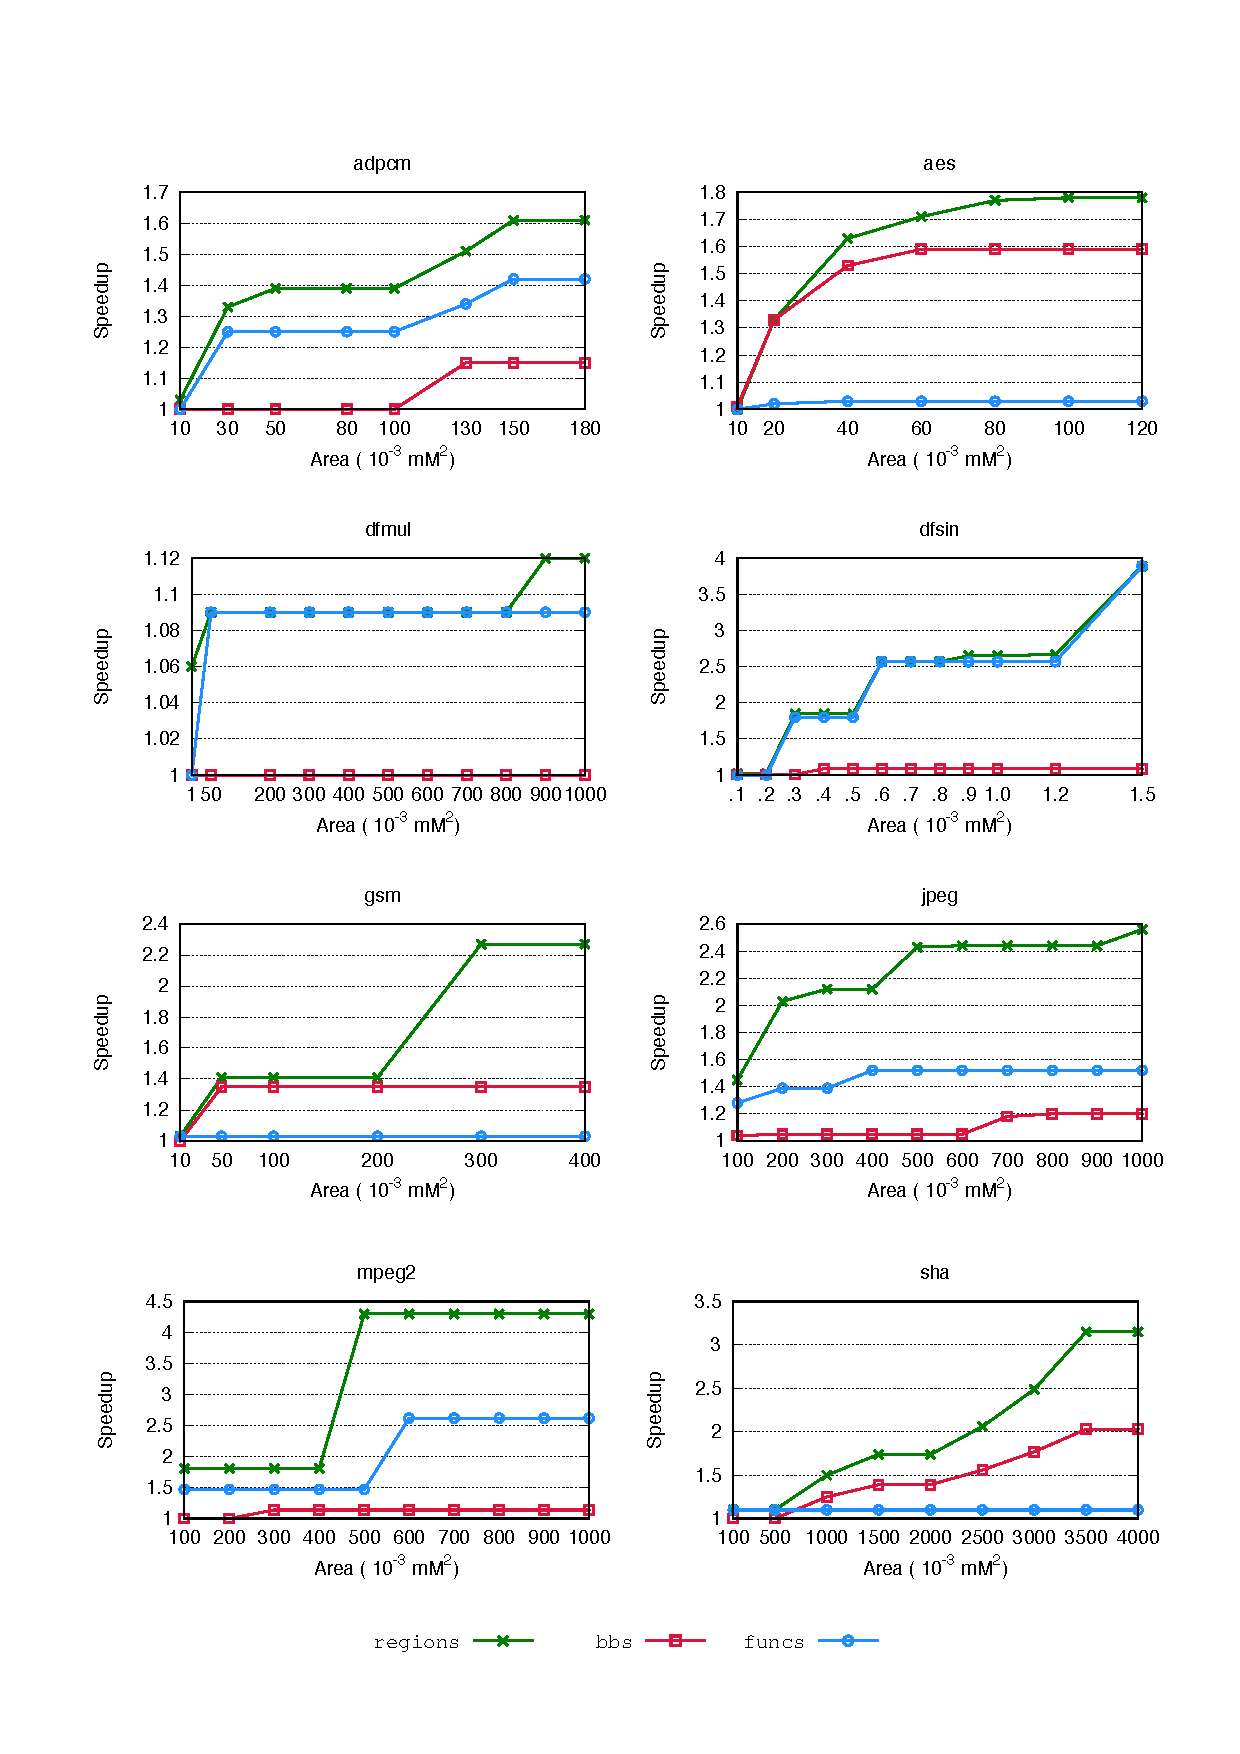
\includegraphics[width= 1.1 \linewidth]{figs/regions_aladdin}
% \caption{Comparison of speedups obtained on eight CHStone benchmarks
%   by selecting regions, only basic blocks and only functions, varying
%   the area constraint, using Aladdin and Gem5 for Speedup and Area evaluation.}
% \label{fig:regions_aladdin}
% \end{figure}

%
% Figures of all Benchmarks simulations - ALADDIN
%%%%%%%%%%%%%%%%%%%%%%%%%%%%%%%%%%%%%%%%%%%%%%%%%%%%%%%%%%%%%%%%%%%%%%%%%%%%%%%%%%
\begin{figure*}
\centering
\subfigure{
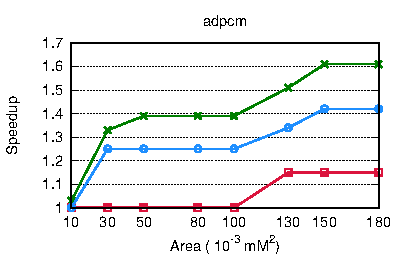
\includegraphics[width=0.44\textwidth]{figs/CHstone_aladdin/adpcm}
}
\subfigure{
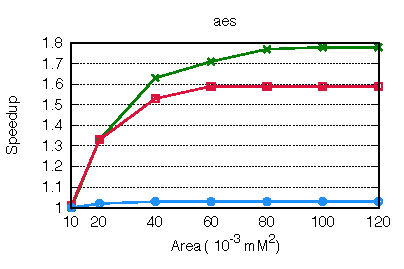
\includegraphics[width=0.44\textwidth]{figs/CHstone_aladdin/aes}
}
\subfigure{
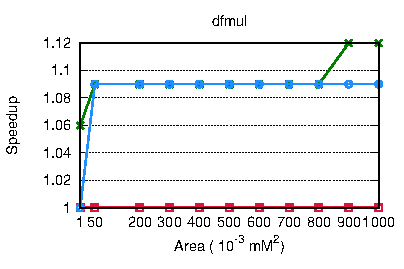
\includegraphics[width=0.44\textwidth]{figs/CHstone_aladdin/dfmul}
}
\subfigure{
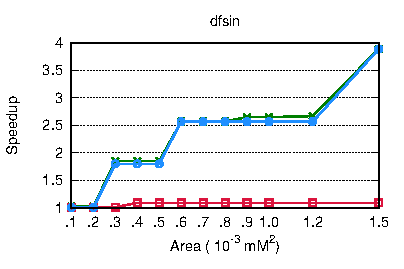
\includegraphics[width=0.44\textwidth]{figs/CHstone_aladdin/dfsin}
}
\subfigure{
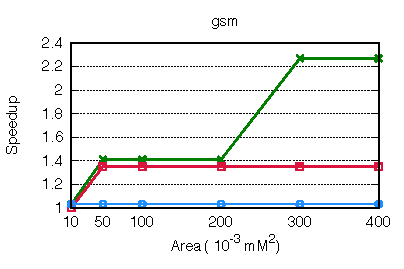
\includegraphics[width=0.44\textwidth]{figs/CHstone_aladdin/gsm}
}
\subfigure{
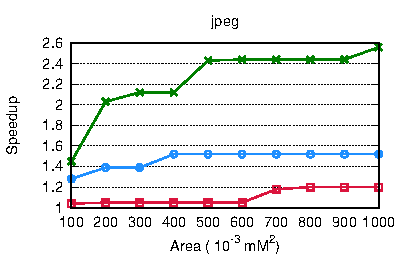
\includegraphics[width=0.44\textwidth]{figs/CHstone_aladdin/jpeg}
}
\subfigure{
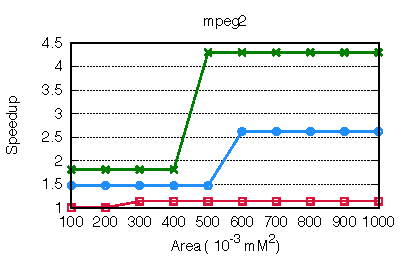
\includegraphics[width=0.44\textwidth]{figs/CHstone_aladdin/mpeg2}
}\subfigure{
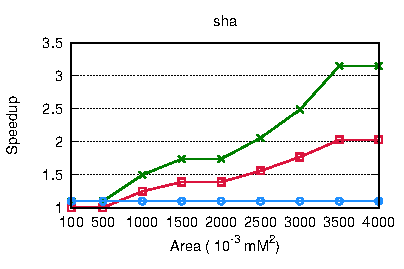
\includegraphics[width=0.44\textwidth]{figs/CHstone_aladdin/sha}
}
\subfigure{
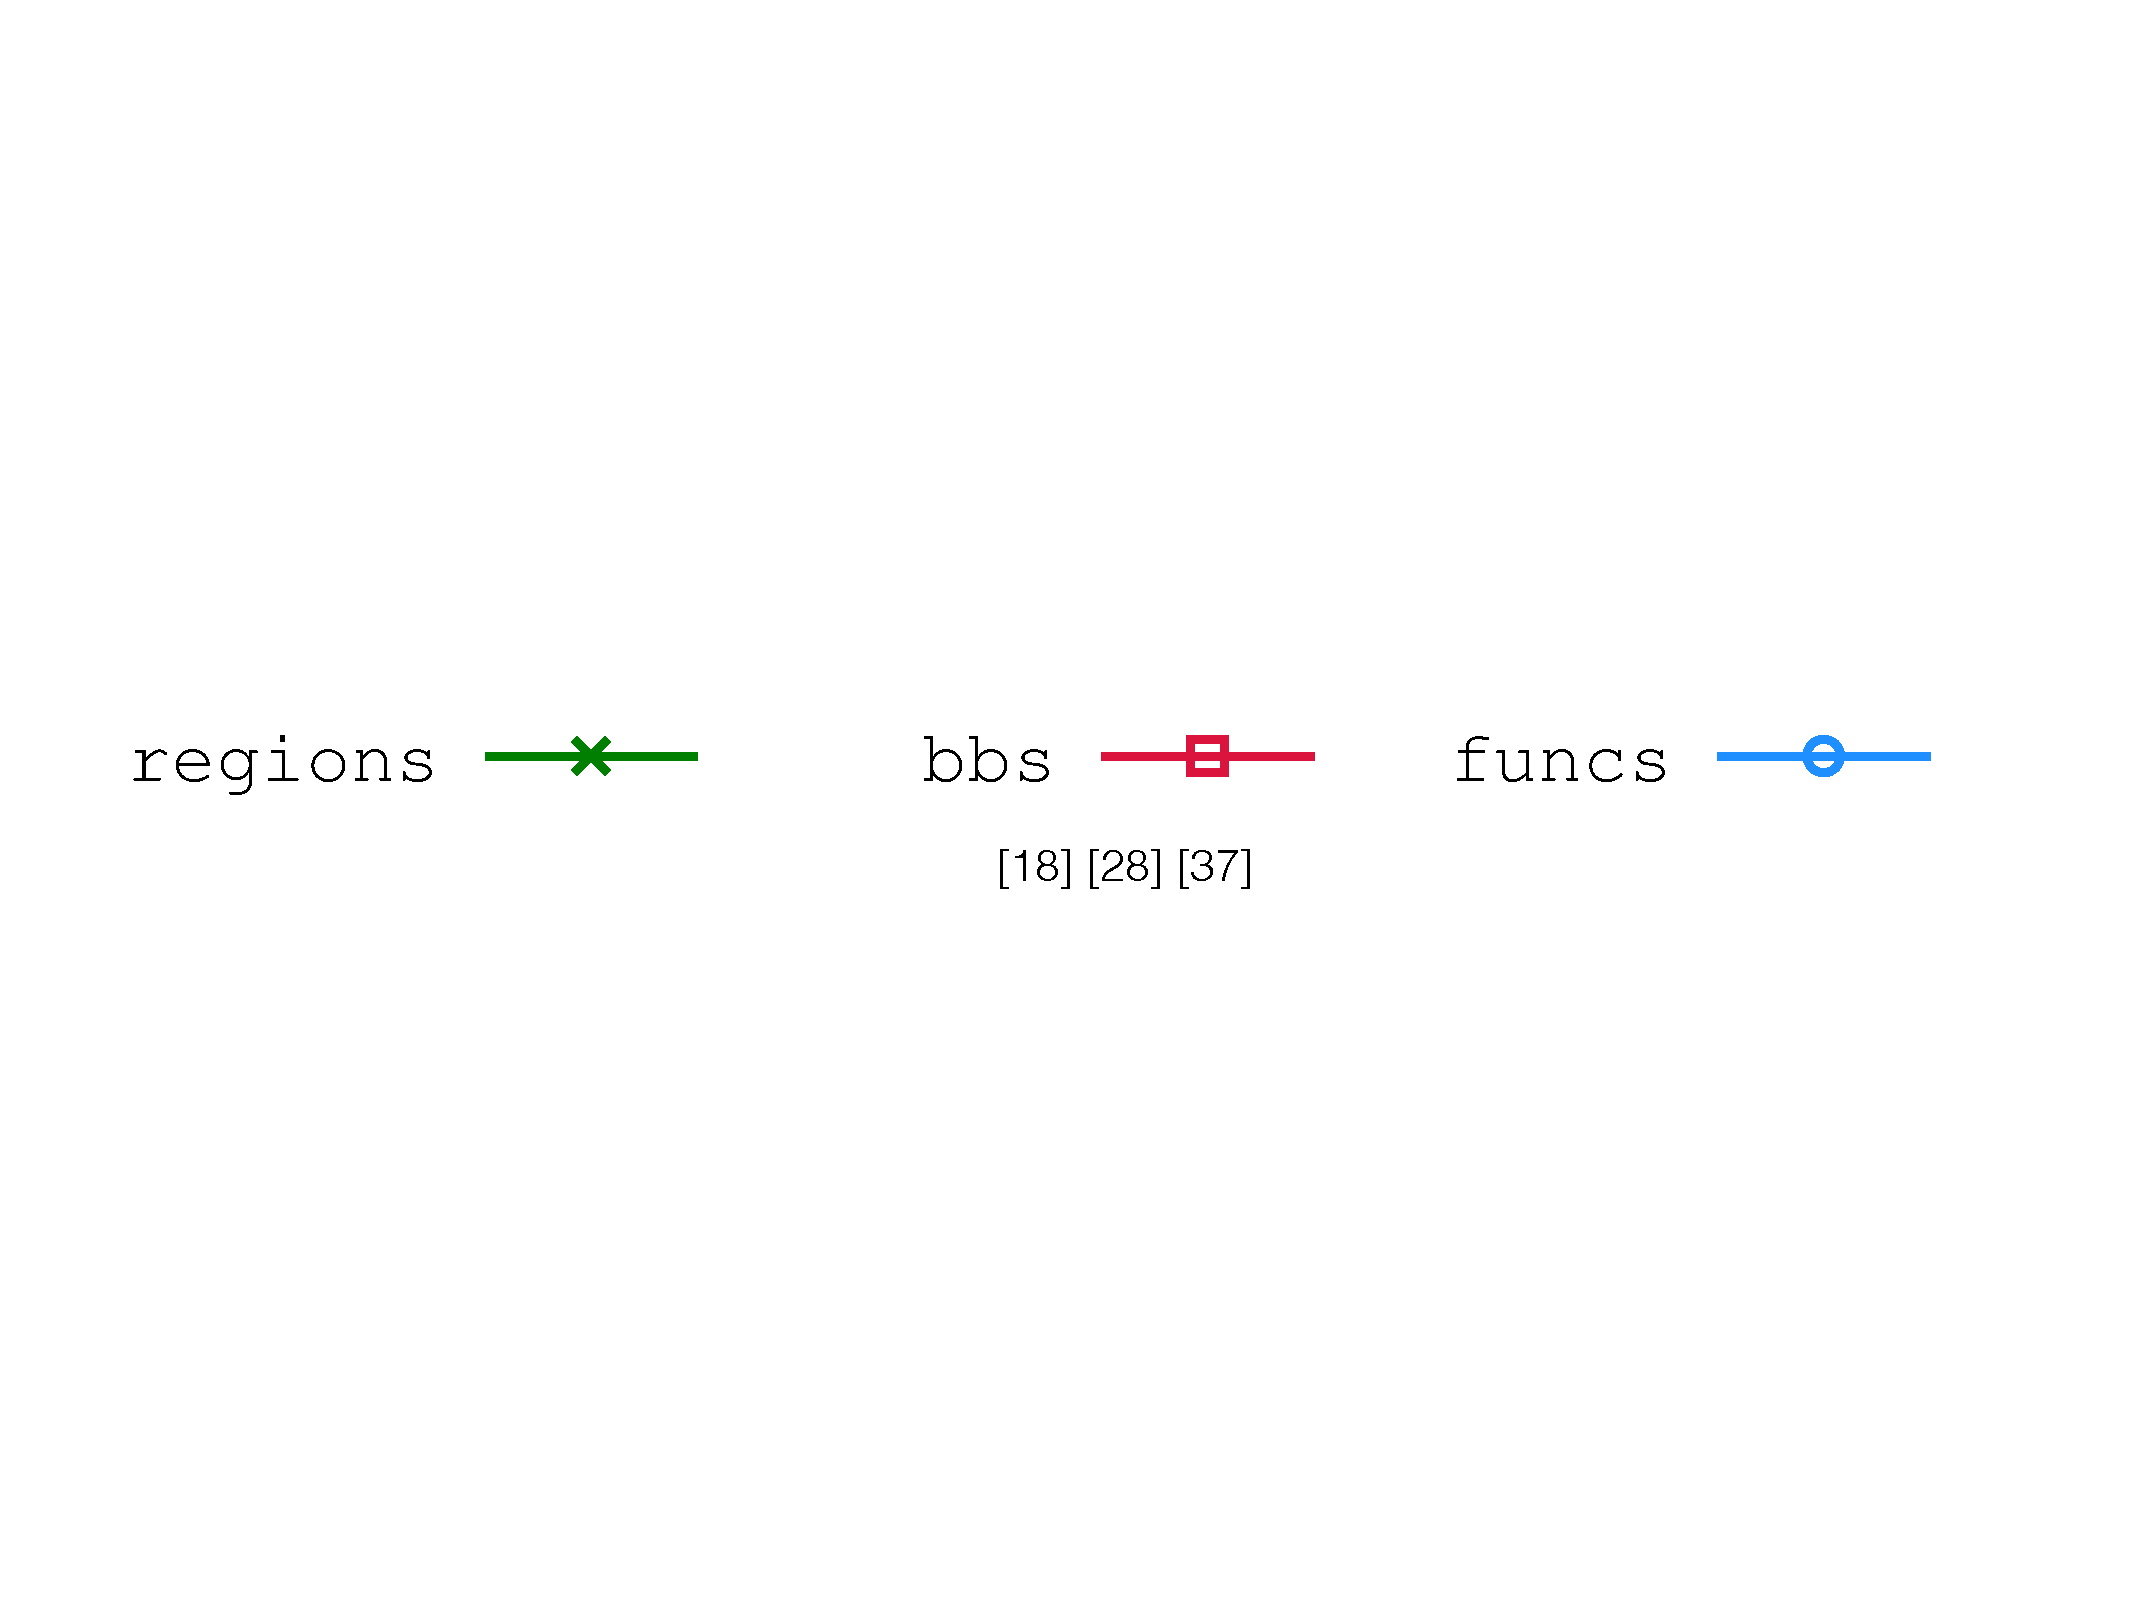
\includegraphics[width=0.44\textwidth]{figs/CHstone/legend}
}
\caption{Comparison of speedups obtained on eight CHStone benchmarks
  by selecting regions, only basic blocks and only functions, varying
  the area constraint, using Aladdin and Gem5 for merit and cost evaluation. }
\label{fig:regions_aladdin}
\end{figure*}

% \begin{figure}[h!]
% \centering
% \hspace*{-1cm}
% 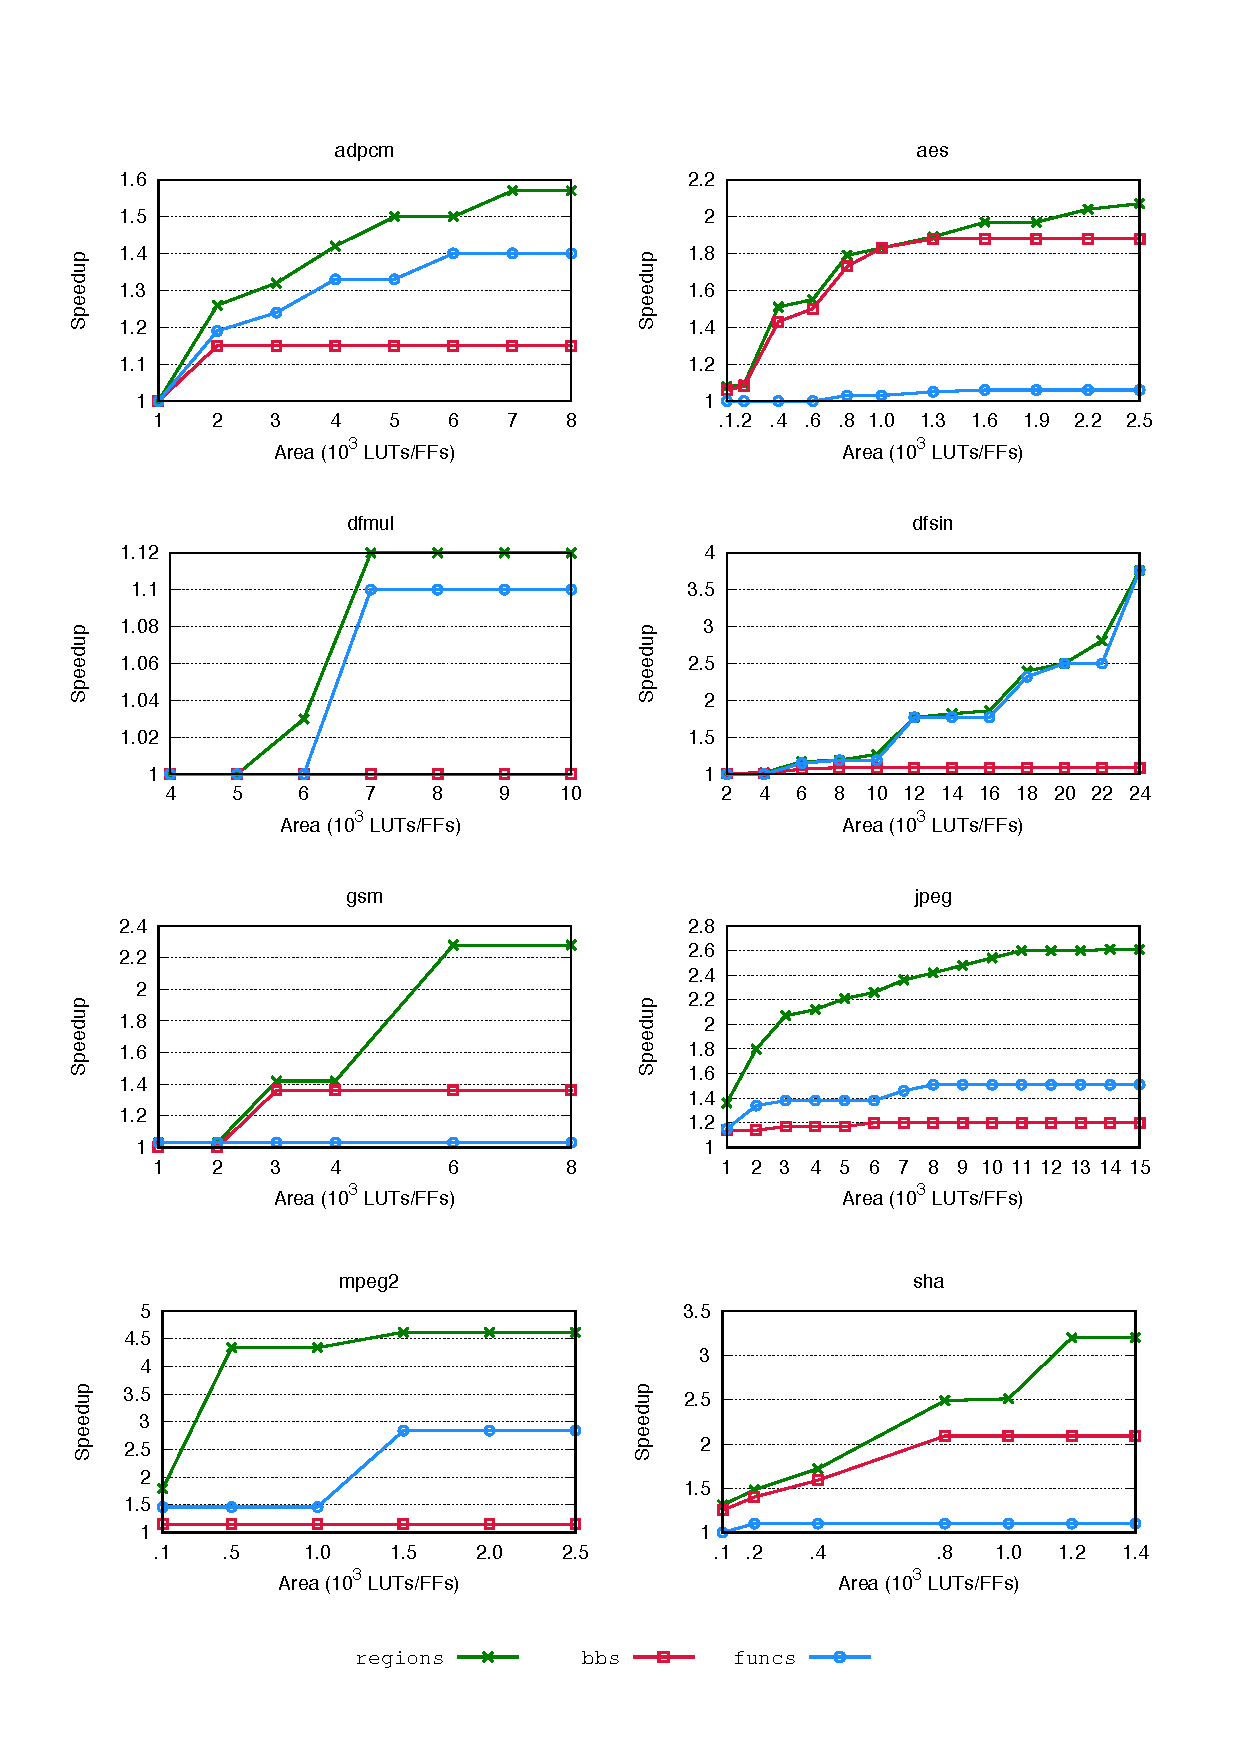
\includegraphics[width= 1.1 \linewidth]{figs/regions_vivado}
% \caption{Comparison of speedups obtained on eight CHStone benchmarks
%   by selecting regions, only basic blocks and only functions, varying
%   the area constraint, using Vivado HLS and Gem5 for Speedup and Area evaluation.}
% \label{fig:regions_vivado}
% \end{figure}

%
% Figures of all Benchmarks simulations.
%%%%%%%%%%%%%%%%%%%%%%%%%%%%%%%%%%%%%%%%%%%%%%%%%%%%%%%%%%%%%%%%%%%%%%%%%%%%%%%%%%
\begin{figure*}
\centering
\subfigure{
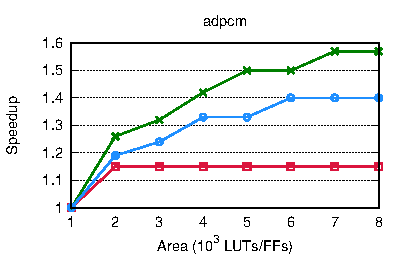
\includegraphics[width=0.44\textwidth]{figs/CHstone/adpcm}
}
\subfigure{
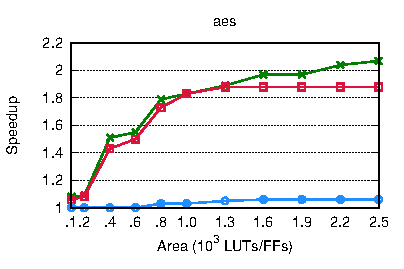
\includegraphics[width=0.44\textwidth]{figs/CHstone/aes}
}
\subfigure{
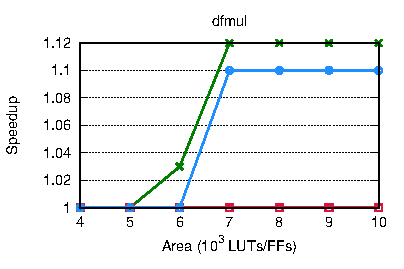
\includegraphics[width=0.44\textwidth]{figs/CHstone/dfmul}
}
\subfigure{
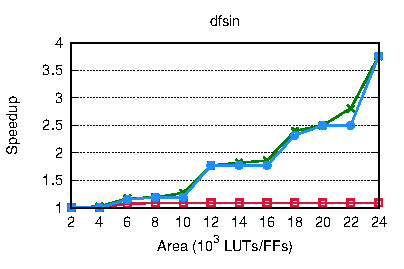
\includegraphics[width=0.44\textwidth]{figs/CHstone/dfsin}
}
\subfigure{
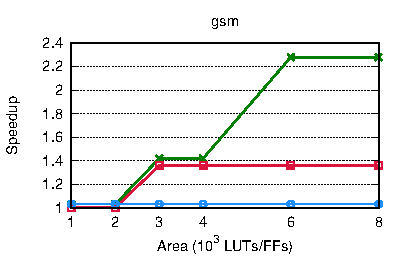
\includegraphics[width=0.44\textwidth]{figs/CHstone/gsm}
}
\subfigure{
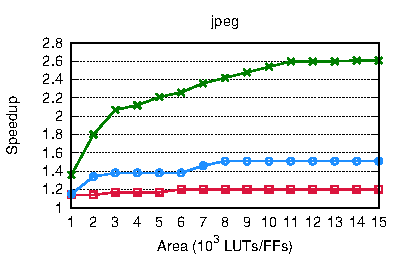
\includegraphics[width=0.44\textwidth]{figs/CHstone/jpeg}
}
\subfigure{
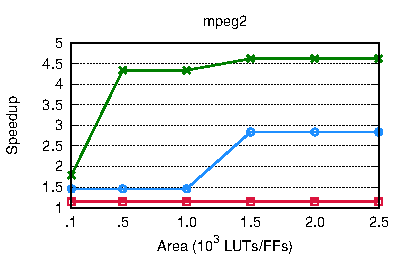
\includegraphics[width=0.44\textwidth]{figs/CHstone/mpeg2}
}\subfigure{
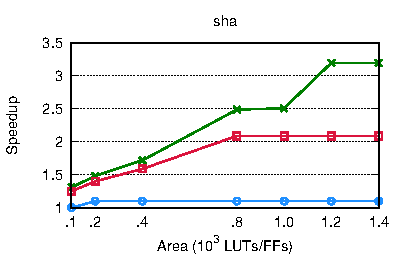
\includegraphics[width=0.44\textwidth]{figs/CHstone/sha}
}
\subfigure{
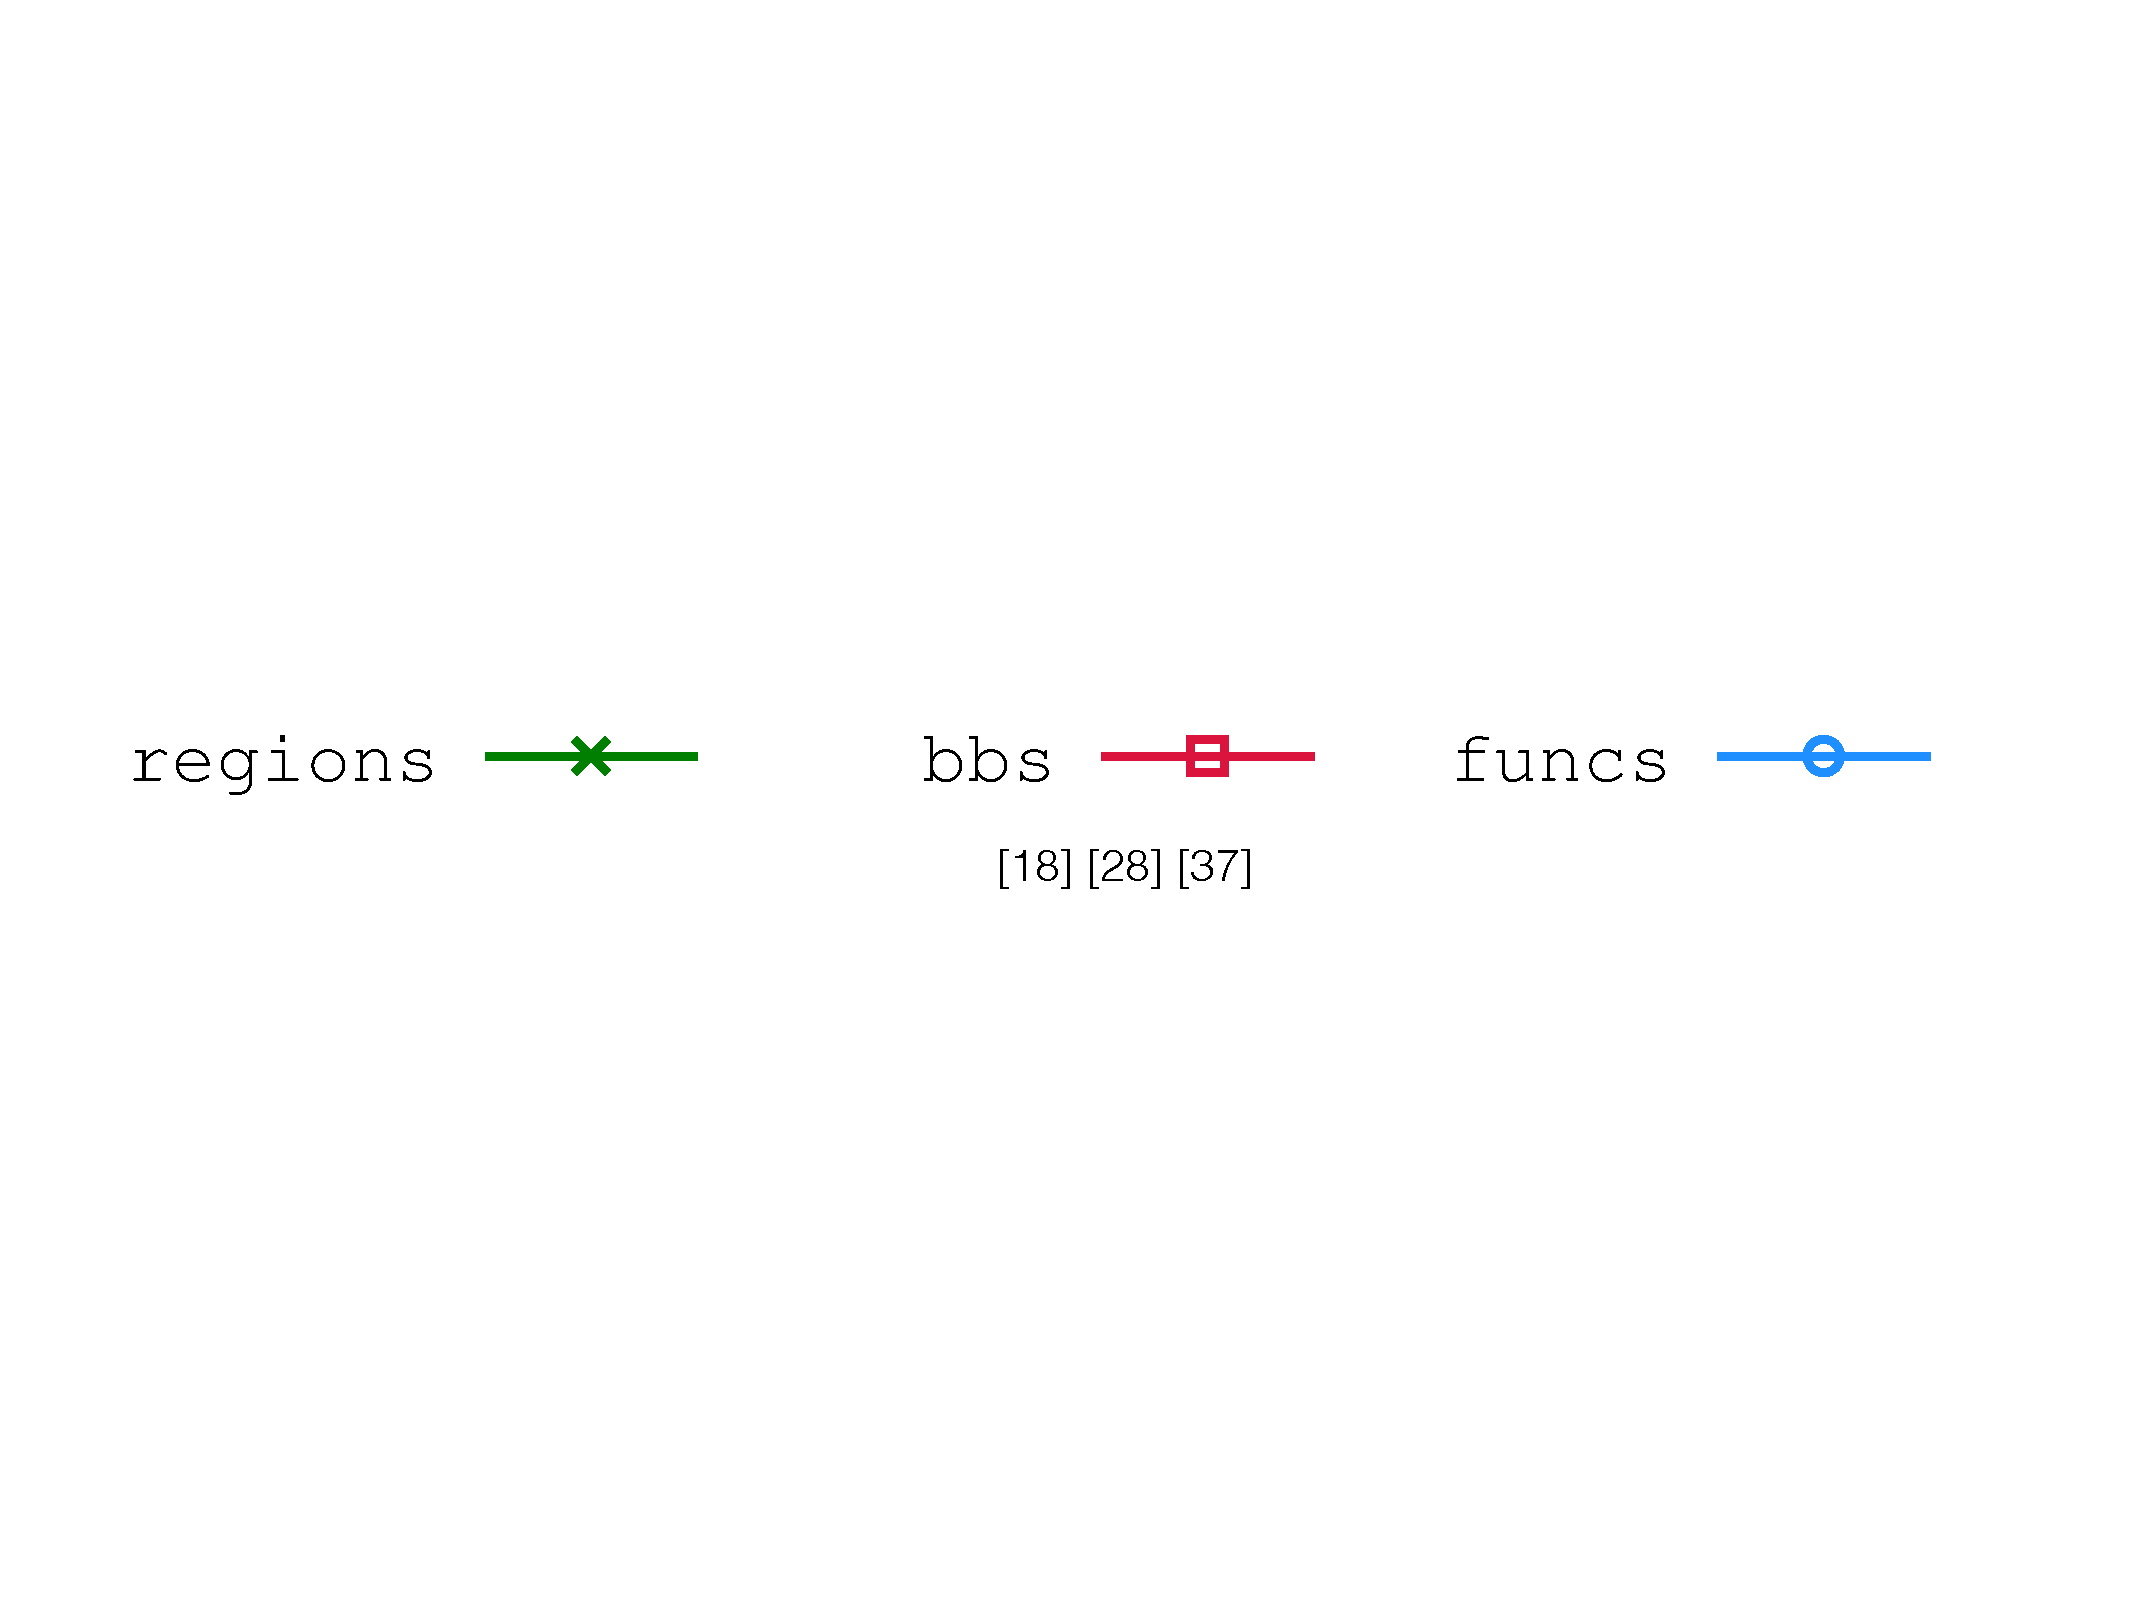
\includegraphics[width=0.44\textwidth]{figs/CHstone/legend}
}
\caption{Comparison of speedups obtained on eight CHStone benchmarks
  by selecting regions, only basic blocks and only functions, varying
  the area constraint, using Vivado\_HLS and Gem5 for merit and cost
  evaluation. }
\label{fig:regions_vivado}
\end{figure*}

\section{Experimental Results}
\label{subsec:exp}

This section investigates and quantitatively assesses the results and
contributions of \rseeker\ from multiple perspectives. First, the speedup 
deriving from considering regions as targets for acceleration is evaluated, 
with respect to \SoTA\ solutions based on functions and basic blocks. Then, the
performance of the algorithms proposed to solve the \rsprobname\ Problem
is analyzed.  Finally, the robustness of region-based acceleration when varying
architectural-specific parameters is explored.\par


\subsection{Regions as a Choice for Accelerators}
\label{subsec:res_llvm}

In order to evaluate the benefits of \rseeker, we comparatively assess
it against two \SoTA\ alternatives.  The first is to
identify accelerators \emph{automatically}, but only within the scope
of \dataflow\ --- which means within the scope of single basic blocks
--- as done by \SoTA\ approaches such as \cite{YuSep04},
\cite{PozziJul06}, \cite{ChenFeb07}, \cite{ReddingtonAug09}, and
\cite{GiaquintaMar15} to name only a few. In particular, the \SoTA\ algorithm 
proposed in \cite{VermaOct07} and used in \cite{PothineniJan07} and in
\cite{GiaquintaMar15} was implemented, that identifies maximum convex subgraphs within
basic blocks. These methods identify the largest part that can be
synthesized and accelerated within a basic block, and hence represent
an upper-bound on the speedup that can be achieved by identification
methods that work at the data-flow (basic block) level. The second is
to mimic the \emph{manual} approach of selecting entire functions,
which is also the scope supported by high-level synthesis tools
\cite{CanisSep13} \cite{VillarrealMay10} \cite{VivadoHLSMar17}.\par

In the experiments, \rseeker\ with the \exactC\ selection method was
used, discarding regions that provide less than 10\% of the maximum
merit. Two sets of experiments were performed: first Aladdin, and then
Vivado HLS were used to estimate merit and cost, highlighting that
the \rseeker\ methodology can be used
% leads to superior results than \SoTA\ methodologies
across different high-level synthesis tools, and more importantly
verifying that the regions selected are largely the same,
independently of the cost and merit estimation model used.\par

Figure~\ref{fig:regions_aladdin} showcases the achieved
speedup, when employing Aladdin, by the accelerators selected by
\rseeker\ (labeled \texttt{regions} in the figure), with respect to
the entire run-time of the applications and for different area
constraints.  For small-to-medium size applications such as \adpcm,
\aes, \gsm\ and \sha\ speedup gains for \rseeker\ vary from 1.6x up to
3.2x. For smaller kernels, larger variations can be observed, as for
\dfmul\ and \dfsin\ the speedup reaches 1.12x and 3.9x respectively.
Finally, for larger benchmarks such as \jpeg\ and \mpeg\, speedup is
fairly significant: 2.5x for the former and up to 4.3x for the latter
can be reached using \rseeker.\par

Similar trends are observed when Vivado HLS is instead used for the
accelerator synthesis, as reported in
Figure~\ref{fig:regions_vivado}: \rseeker\ consistently outperforms
\SoTA\ approaches which target either single basic blocks or
entire functions, across all benchmarks. These results 
highlight that the achievable speedups
are highly influenced by which segments of applications are selected
for accelerations, and that such choice is only marginally influenced
by the adopted merit and cost estimation tool. In fact, it was verified
that across the two sets of experiments, the regions chosen were
\emph{the same} in 80\% of the cases. As an example, out of 10 regions
selected to achieve a 2.2x speedup for the \jpeg\ benchmark, 8 are the
same when using either Aladdin or Vivado HLS for merit and cost
estimation, and the ones that differ contribute to less than 14\% of
the provided gain.\par

The speedup that can be obtained by accelerating basic blocks is
hampered by their small granularity and, consequently, the high number
of switches between software and hardware execution. Moreover, in this
setting many optimization opportunities
during the hardware implementation of the accelerators are missed,
because they only arise when control flow is considered, as is instead the case
for regions.
On the other hand, the speedup derived by selecting whole functions
trails the one corresponding to regions, because of two
reasons. First, function selection is limited to the ones which do not
present forbidden nodes, and this might rule out promising regions
within them. Second and more importantly, it is also inflexible from
an area viewpoint, which is especially visible when few hardware
resources are available for acceleration. In those cases, the
selection of functions often detects only few feasible candidates,
with a small merit (e.g., in \jpeg\ and \mpeg, for an area of less
than 0.5 $mM^2$).\par

This limitation is not present for regions, as only the part
pertaining to individual hotspots inside a function can be
selected. Indeed, the performance of \rseeker\ stems from the high
flexibility of the selection approach, as it allows the consideration of
the entire spectrum of granularity ranging from whole functions to
single loops, ultimately enabling a better exploitation of speedup for
a given area budget.

\begin{figure}[h]
\centering
%\hspace*{-2cm}
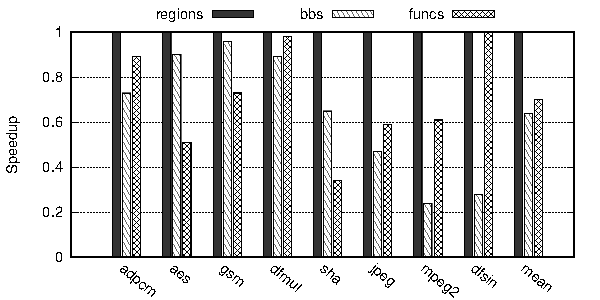
\includegraphics[width= 0.8 \linewidth]{figs/rbf_max_norm_all}
\caption{Normalized Speedup of RegionSeeker with respect to function and basic block selection, 
considering, for each benchmark, a fixed area constraint. Synthesis performed with Vivado HLS.}
\label{fig:regions_all}
\end{figure}

A summary of the performed experimental exploration is presented in
Figure \ref{fig:regions_all}.  It reports the normalized speedups
obtained by \rseeker\ compared to basic block and function
identification, when the maximum considered area budget and
Vivado\_HLS are employed.  The rightmost column set illustrates that,
on average, \rseeker\ harnesses approximately 30\% higher speedups
with respect to the two baseline methods. Moreover, while in some
cases the baselines match the performance of \rseeker\ (e.g.: \gsm\
for basic blocks, \dfsin\ for functions), neither of them can do that
consistently across different area constraints and across
applications, showcasing the suitability of control-flow regions as
accelerator candidates.

\subsection{Performance of Selection Algorithms}
\label{subsec:algo-perf}

In Section~\ref{sec:rs_algos}, three selection algorithms were presented:
an exact algorithm that might not scale for large benchmarks, a naive
greedy, and a meet-in-the-middle approach where the exact algorithm is
applied only to a cropped list of regions, as opposed to all regions
of a benchmark. In this section, the performance of these algorithms
is evaluated, in terms of scalability and of goodness of the solution
found.\par

\begin{figure*}[h]
\centering
  \hspace*{-2cm}
\subfigure{
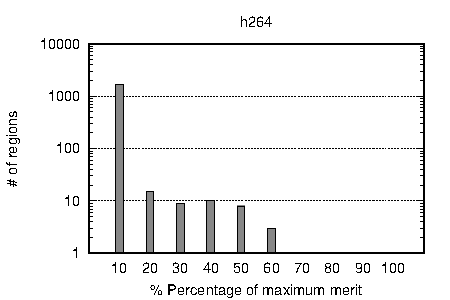
\includegraphics[width=0.5\textwidth]{figs//h264-reg.pdf}
\label{fig:h264-reg}
}
\subfigure{
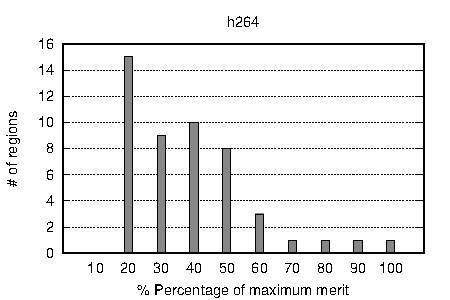
\includegraphics[width=0.5\textwidth]{figs//h264-pr-reg.pdf}
\label{fig:h264-pr-reg}
}
  \hspace*{-2cm}
\caption{Left: The \numofhtsfregs\ regions of \htsf\ are partitioned here
  in ten bins, according to their merit $M()$. Regions providing up to
  10\% of the maximum merit fall in the first bin, from 10\% to 20\%
  in the second bin etc. Notice that the distribution is extremely
  skewed.  Right: The nine most profitable bins are here shown in linear
  scale, for clarity.  The skewness of this distribution is leveraged
  by the \exactC\ selection algorithm.  }
\label{fig:h264-regions}
\end{figure*}

To this end, a complex benchmark is targeted (namely, \htsf\
\cite{H264May15}), which has a code size of more than ten thousand
lines of code and contains thousands of regions. Note that, while
Aladdin provides merit and cost estimation for a region very quickly
(a matter of milliseconds per region) and therefore could have been
employed for this experiment of algorithm scalability, it does,
however, require the outlining of the selected accelerator
specifically \emph{as a function call} within the application source
code --- and this currently needs to be done manually. This technical
limitation means that Aladdin estimations cannot be used for the
scalability experiments in this section.
Hence, a more abstract model was employed, which could be implemented
directly within the LLVM toolchain, relying on the LLVM intermediate
representation and without needing manual intervention on benchmark
source code. The cost of a region was estimated as the area required to
implement its DFG nodes, and its merit as the cycles saved between SW
and HW execution, where the latter is the delay of the nodes on the
DFG critical paths, each multiplied by their respective frequency.\par


Firstly, in Figure \ref{fig:h264-regions} it is shown, for the \htsf\
benchmark, the distribution of all regions with respect to their merit
$M()$.
It becomes apparent in this figure that the distribution is extremely
skewed, with very few regions having high merit and the majority
providing a negligible one. This is to be expected, as it is well
known that a large percentage of time, in running a software
application, is typically spent on a small percentage of code. And of
course a region merit is proportional to the frequency of execution of
its corresponding code segment.\par

\begin{figure}[t]
\centering
\hspace*{-2cm}
\subfigure{
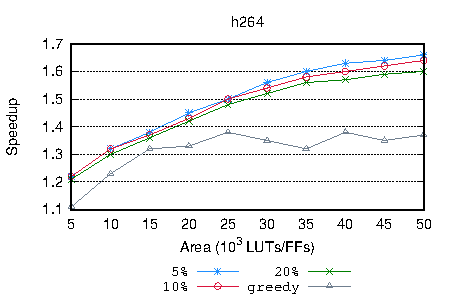
\includegraphics[width=0.5 \textwidth]{figs/ex_gr_speed_h264}
\label{fig:h264-speed}
}
\subfigure{
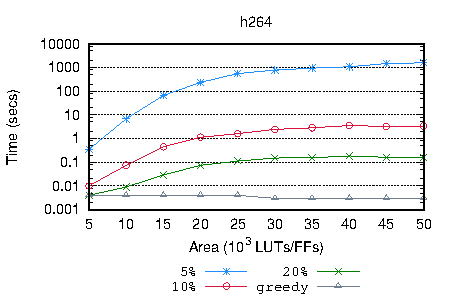
\includegraphics[width=0.5 \textwidth]{figs/ex_gr_time_h264}
\label{fig:h264-time}
}
\hspace*{-2cm}
\caption{Left: Speedup achieved on the \htsf\ benchmark by \exactC,
  cropped by considering only regions providing at least 5\%, 10\% and
  20\% of the maximum merit, and by \greedy.  Right: Corresponding
  algorithms execution time.}
\label{fig:h264-ex-gr}
\end{figure}

% Region h264 Exact Versions.
\begin{figure}[h]
\centering
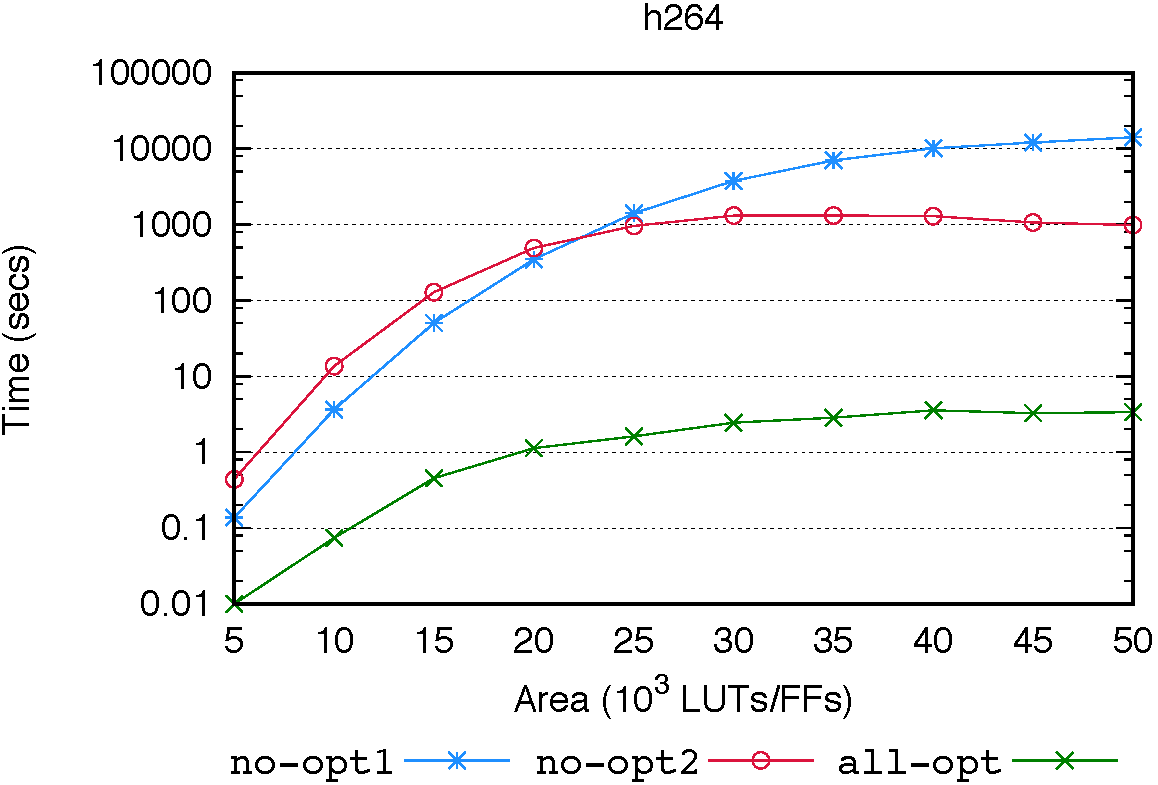
\includegraphics[width=0.6\textwidth]{figs/exact_versions}
\caption{Execution time of the \exactC\ algorithm (cropping
  level at 10\%), when the two optimizations described in subsection
  \ref{sec:algo-exact} are removed.  }
\label{fig:h264-exact-versions}
\end{figure}

For a large benchmark such as \htsf, the \exact\ algorithm does not
scale if it is fed all \numofhtsfregs\ regions. However, it is reasonable
to expect that, given the distribution seen, the goodness of the
solution found should decrease only slightly when discarding a large
number of low-potential regions, while scalability
could grow tangibly.
This assumption is confirmed by the data in
Figure~\ref{fig:h264-ex-gr}, where the comparison of performance and
scalability of the \exactC\ selection algorithm is performed, at three different
levels of cropping --- that is, considering regions providing at
least 5\%, 10\% and 20\% of the maximum merit, respectively.\par

Figure~\ref{fig:h264-ex-gr} (left) plots the estimated speedup achieved by
implementing a set of regions in hardware, selected by the three \exactC\
levels, and by \greedy, for different area constraints. It can be seen
that, when changing the level of cropping, the goodness of the
solutions found by \exactC\ differs only slightly (as expected, little
is lost when some low-potential regions are ignored) and it is
altogether largely superior to fast but naive \greedy.\par

However, as a second issue worth observing, the exploration space for
the three different levels of cropping differs greatly, and hence the
time spent by each of these algorithms to terminate. This can be seen
in Figure~\ref{fig:h264-ex-gr} (right) : orders of magnitude separate
the time spent by each, with \exactC\ at 5\% taking hours, and at 10\%
taking seconds.\par

Last, the effect of the optimizations that were devised for
improving search tree exploration is shown. These optimizations were 
described in Section~\ref{sec:algo-exact} and exemplified in
Figure~\ref{fig:exact_tree}. They are 1: pruning the
exploration tree when a certain best merit, found so far, cannot be
reached, and 2: processing regions in order of decreasing merit. In
Figure~\ref{fig:h264-exact-versions} it can be seen how the two
optimizations affect the algorithm run time. When pruning is turned
off, more than three orders of magnitude are lost, in time. When the
list of regions is processed in an order different than that of
decreasing merit (in this experiment, an order of decreasing
\emph{density} is considered, i.e. \emph{merit divided by cost}) more
than two orders of magnitude are lost.

\subsection{Impact of the Interface Overhead}
\label{subsec:res_overhead}

The initiation of an accelerated routine on a dedicated hardware block
always entails a timing penalty $T_{Overhead}$.  Such overhead is
highly dependent on the interface protocol between the processor and
the application-specific accelerators. While the definition of such
protocol is outside the scope of this work, the
impact of adopting different values for this parameter is worthy to investigate, 
when different selection methods are employed.\par

Two observations can be made by analyzing the results of Figure
\ref{fig:overhead}, reported for the \sha\ benchmark. Firstly, the speedup 
obtained by \rseeker\ is not
affected in any significant way by the variation of the value of
$T_{Overhead}$ among one, ten and twenty cycles, while the speedup for
basic blocks is indeed affected. This is to be expected, since basic
block level accelerators require a higher number of invocations (e.g.:
for each iteration of an intensive loop) than region-level
accelerators. Secondly, while by decreasing the value of
$T_{Overhead}$ the speedup of basic block increases, it does not
increase in a significant way and is still %much
less tangible than the speedup achieved by \rseeker.

\begin{figure}[h]
\centering
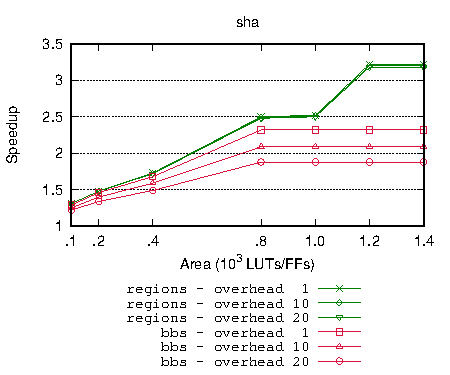
\includegraphics[width=0.6 \linewidth]
{figs/overhead_sha}
\caption{Impact of the initiation overhead for regions and basic
  blocks selection strategies, considering $T_{Overhead}$ values of 1,
  10, and 20 clock cycles.}
\label{fig:overhead}
\end{figure}



% OLD START
%
%
%
%

% Figure~\ref{fig:regions_aladdin} showcases the achieved
% speedup, when employing Aladdin, by the accelerators selected by
% \rseeker\ (labeled \texttt{regions} in the figure), with respect to
% the entire run-time of the applications and for different area
% constraints.  For small-to-medium size applications such as \adpcm,
% \aes, \gsm\ and \sha\ speedup gains for \rseeker\ vary from 1.6x up to
% 3.2x. For smaller kernels, larger variations can be observed, as for
% \dfmul\ and \dfsin\ the speedup reaches 1.12x and 3.9x respectively.
% Finally, for larger benchmarks such as \jpeg\ and \mpeg\, speedup is
% fairly significant: 2.5x for the former and up to 4.3x for the latter
% can be reached using \rseeker.\par

% \begin{figure}[h!]
% \centering
% \hspace*{-1cm}
% 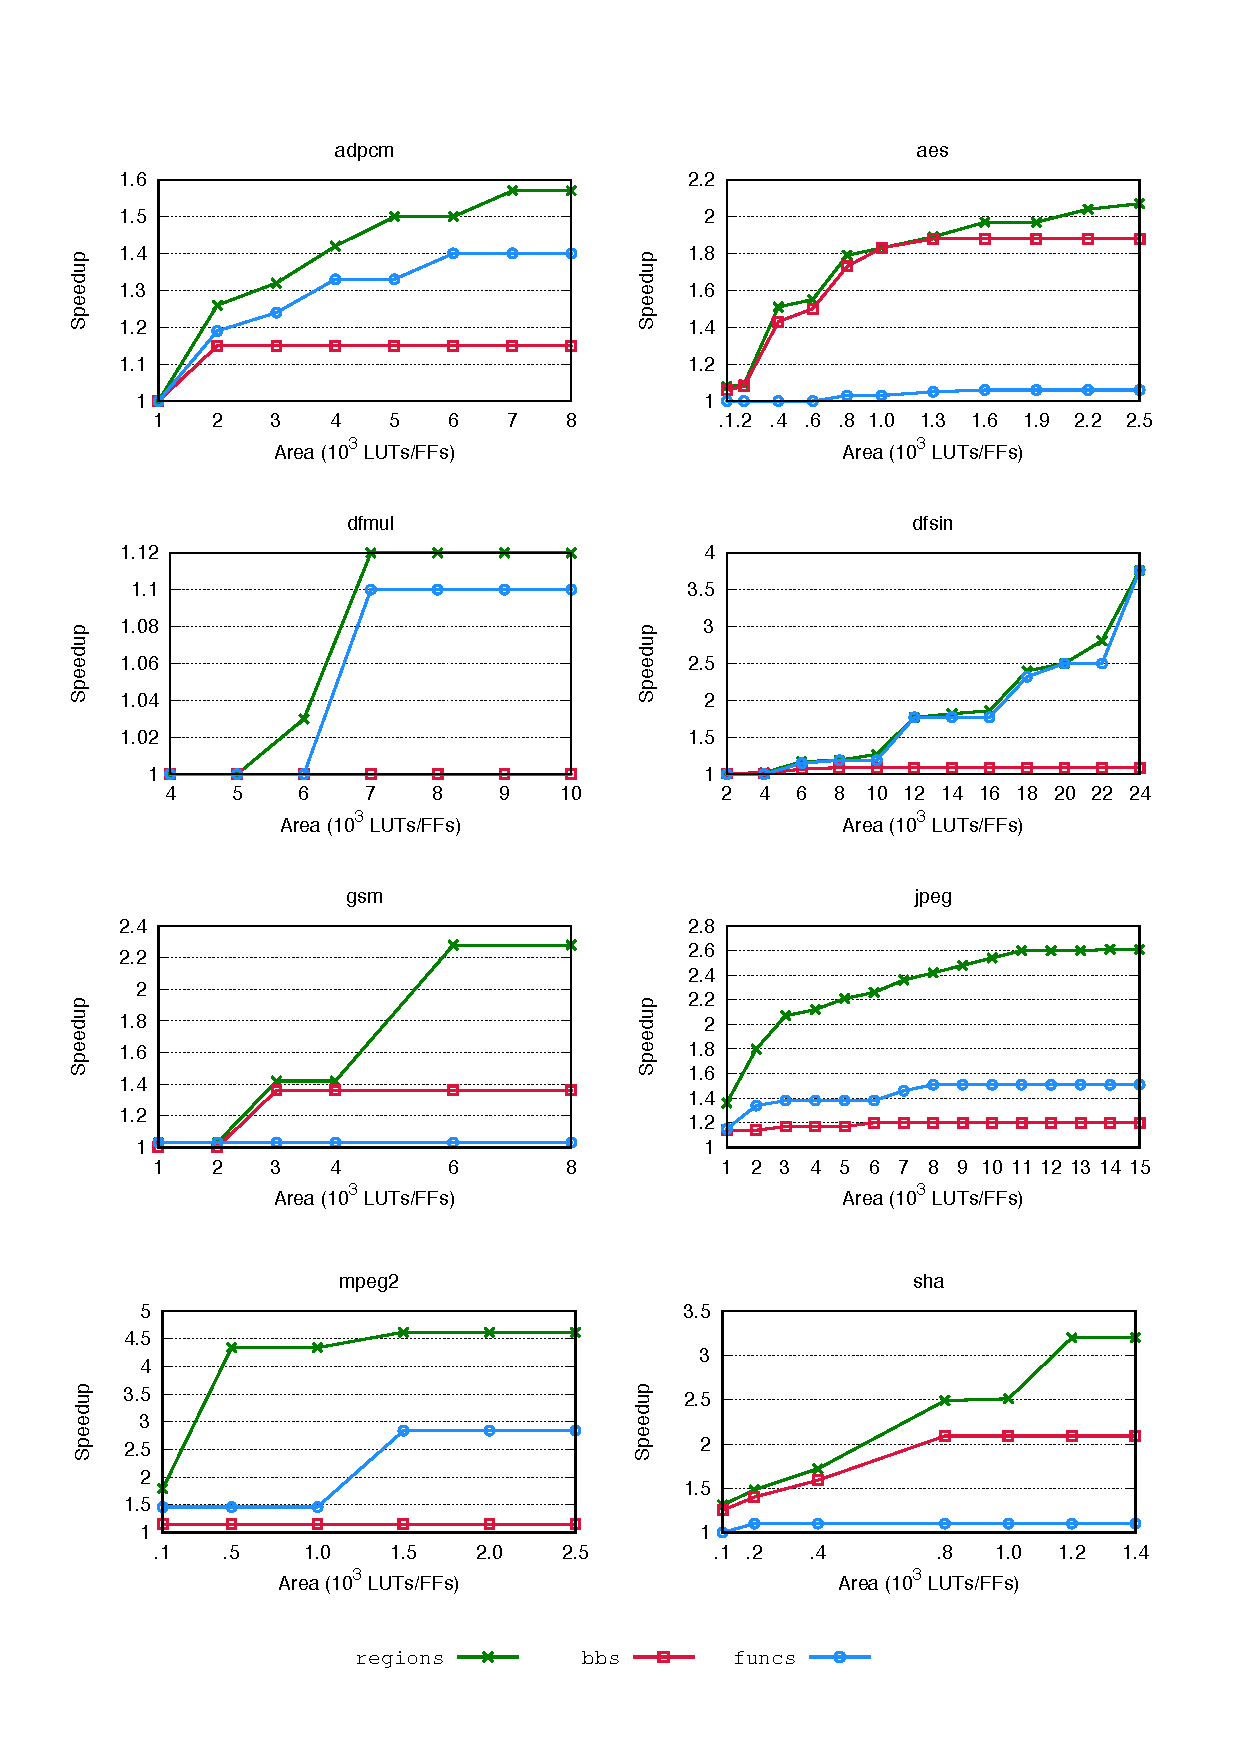
\includegraphics[width= 1.1 \linewidth]{figs/regions_vivado}
% \caption{Comparison of speedups obtained on eight CHStone benchmarks
%   by selecting regions, only basic blocks and only functions, varying
%   the area constraint, using Vivado HLS and Gem5 for Speedup and Area evaluation.}
% \label{fig:regions_vivado}
% \end{figure}

% Similar trends are observed when Vivado HLS is instead used for the
% accelerator synthesis, as reported in
% Figure~\ref{fig:regions_vivado}: \rseeker\ consistently outperforms
% \SoTA\ approaches which target either single basic blocks or
% entire functions, across all benchmarks. These results 
% highlight that the achievable speedups
% are highly influenced by which segments of applications are selected
% for accelerations, and that such choice is only marginally influenced
% by the adopted merit and cost estimation tool. In fact, this was verified 
% across the two sets of experiments, as the regions chosen were
% the same in 80\% of the cases. As an example, out of 10 regions
% selected to achieve a 2.2x speedup for the \jpeg\ benchmark, 8 are the
% same when using either Aladdin or Vivado HLS for merit and cost
% estimation, and the ones that differ contribute to less than 14\% of
% the provided gain.\par


% \begin{figure}[h]
% \centering
% %\hspace*{-2cm}
% 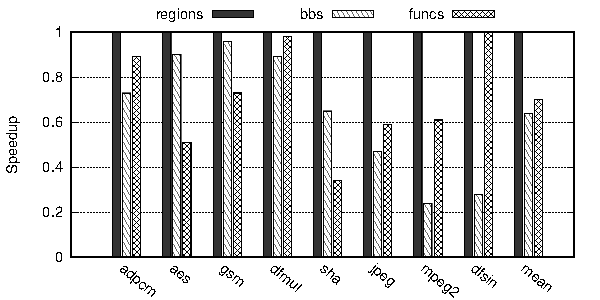
\includegraphics[width= 0.9 \linewidth]{figs/rbf_max_norm_all}
% \caption{Normalized Speedup of RegionSeeker with respect to function and basic block selection, 
% considering, for each benchmark, a fixed area constraint. Synthesis performed with Vivado HLS.}
% \label{fig:regions_all}
% \end{figure}

% Finally, in Figure \ref{fig:regions_all} a summary of the performed experimental 
% exploration is presented. It reports the normalized speedups
% obtained by \rseeker\ compared to basic block and function
% identification, when a fixed area budget is considered and
% Vivado HLS are employed. The mean column illustrates that,
% on average, \rseeker\ achieves approximately 30\% higher speedups
% with respect to the two baseline methods. Moreover, while in some
% cases the baselines match the performance of \rseeker\ (e.g.: \gsm\
% for basic blocks, \dfsin\ for functions), neither of them can achieve that
% consistently across applications, stressing the suitability of control-flow regions as
% HW accelerator candidates.\par

% The speedup that can be obtained by accelerating basic blocks is
% hindered by their small granularity and, consequently, the high number
% of HW accelerators invocations by the SW processor, i.e., the switches 
% between software and hardware execution. Moreover, in this
% setting many optimization opportunities
% during the hardware implementation of the accelerators are missed,
% because they only arise when control flow is considered, as is instead the case
% for regions.\par

% On the other hand, the speedup derived by selecting whole functions
% trails the one corresponding to regions, because of two
% reasons. First, function selection is limited to the ones which do not
% present forbidden nodes, and this may rule out promising regions
% within them. Second and more importantly, it is inflexible from
% an area viewpoint, which is especially visible when few hardware
% resources are available for acceleration. In those cases, the
% selection of functions often detects only few feasible candidates,
% with a small merit (e.g. in Figure \ref{fig:regions_aladdin}: \jpeg\ and 
% \mpeg, for an area of less than 0.5 $mM^2$).\par

% This limitation, though, is not present in regions, as simply the part
% referring to individual hotspots inside a function can be available
% for selection. Indeed, the performance of \rseeker\ stems from the high
% flexibility of the selection approach, as it allows the consideration of
% the entire spectrum of granularity ranging from whole functions to
% single loops, ultimately enabling a better exploitation of speedup for
% a given area budget.

% OLD END!
%
%
%
%

\newpage
%
%
%     RegionSeeker MuLTiVersioning
%
%
%
%
\section{RegionSeeker MuLTiVersioning}
\label{sec:multi}

\HLS\ (HLS) tools, such as Vivado HLS by Xilinx, may employ %additional 
optimizations to HW accelerators
design in order to increase performance, i.e. obtain faster execution. 
To support different optimization levels, an extension of \rseeker\ framework 
is presented in this section, 
% These 
% %pragma-directed 
% HLS optimizations were not taken into account by \rseeker\ framework in the
% previous section. Default, non optimized versions of HW accelerators were identified
% and selected instead. 
% In this
% section an extended \rseeker\ framework is presented, which 
which performs the selection not 
only among possible CFG subgraphs, but also among different versions of each identified 
subgraph, namely different versions of the regions identified. 
This extension is referred to in the rest of the document as RegionSeeker: the 
MuLTiVersioning approach.

% The \rseeker\ framework, as detailed in the previous section, was designed in order to identify
% the most efficient HW accelerators under a given constraint, but was targeting default HW
% implementations. Pragma-directed HLS optimizations were not taken into account. In this 
% section we present an extended \rseeker\ framework, which performs the selection not 
% only among possible CFG subgraphs, but also among different versions of each identified 
% subgraph of the CFG, namely different versions of the regions identified. 
% We call this extension the RegionSeeker: MuLTiVersioning approach.

\subsection{Methodology}
\label{subsec:mv_meth}

The rationale, supporting the extension of \rseeker\ framework, is to achieve improved
speedup by exploiting a more varied set of HW accelerators to select from, 
with different optimizations implemented onto them. This goal is being achieved by instantiating 
different versions of each HW accelerator with the same functionality, yet different speedup gains 
and different area (HW resources) requirements. The set of optimizations that were considered in 
order to design different HW implementations of the same accelerators are: 
\begin{enumerate}
\item The Loop Unrolling 
(LU) factor, in accelerators that contain loops.
\item The loop pipelining option, being either on or off.
\item The array partition factor, 
which is the number of input and output ports of the memory buffer (scratchpad) attached 
to the accelerator.
\end{enumerate}\par

Loop unrolling optimization is an HLS directive that, in the context of \HLS\, instantiates multiple 
copies of the logic implementing the functionality defined in a loop body, drastically impacting the 
performance of HW accelerators \cite{KurraApr07} \cite{KulkarniOct12}. This directive can be applied in HW
accelerators containing loops whose trip count can be statically defined. It should nonetheless
be applied in a careful manner, as it entails a high area cost for the duplicated logic. Furthermore,
the resulting benefits can be hampered by frequent memory accesses and loop-carried dependencies, which 
impose a serialization of the run-time execution, thus negating any benefits resulting from loop unrolling.\par

Loop pipelining is an additional HLS directive applied in loops that allows the pipelining of 
the operations contained in a single body of a loop and across consecutive iterations. Restrictions 
regarding loop-carried dependencies across consecutive iterations can also limit the application of the loop
pipelining optimization as the result of the output of a loop iteration would be required in the following
one, thus not allowing the pipelining of the loop body operations.\par

Given an initial set of HW accelerators, i.e., a set of regions that is derived by the \rseeker\ framework, 
multiple versions for each region can be generated that maintain the same functionality.
Each version may employ one of the optimizations listed above, or a combination of them.
\par

All versions of the HW accelerators were evaluated by the Aladdin HW accelerator simulator.  
Aladdin targets ASIC implementations. It provides a fast evaluation, but does not generate a 
synthesizable netlist,
as opposed to Vivado HLS. Nonetheless, the estimations provided are
within 1\% of the ones derived from a Register-transfer level (RTL) implementation, according to 
the developers of Aladdin \cite{ShaoJul14}.
For all simulated versions of the selected regions (or HW accelerators), the number of Cycles and number 
of Functional Units (FU) Area were retrieved. For the SW execution time the gem5 simulator 
\cite{BinkertFeb11}
was used with two CPU settings: a) TimingCPU  (a simple and slow CPU with only two pipeline stages)
and b) O3CPU (a complex and fast CPU with five pipeline stages and other resources such as a 
branch predictor, reorder buffer etc). \par


The \exact\ selection algorithm, as detailed in Subsection \ref{sec:algo-exact}, was used subsequently 
to perform the subset selection that maximizes speedup, 
given an initial set of HW accelerators along with their respective versions, as well as a specific 
area (HW resources) budget. An important note is that no more than one version of each candidate 
can be selected, as only one realization of the respective SW execution is required.
To ensure that, each version is marked with the same set of basic block indexes and the selection
takes place by considering the overlapping graph presented in Figure \ref{fig:exact_tree}.
As a result multiple versions of the same region cannot be selected during the selection phase as this 
would violate the first condition of the \rsprobname\ problem as defined in Subsection \ref{sec:prob}.

% To ensure that, the selection took place utilizing the overlapping graph presented in Figure \ref{fig:exact_tree} 
% containing the basic block indexes included in each region. As a result the set of basic block indexes for 
% multiple versions of the same region would be identical.
% Experiments were run in \jpeg\ benchmark and four different selection
% approaches are presented, comparing three of them to the \multi\ approach.\par

\subsection{Experimental Results}
\label{subsec:mv_res}

The experimental setup was the same as in the \rseeker\ framework, with a system comprising a single 
SW processor and multiple loosely coupled HW accelerators, exchanging shared data with \plms.
The processor invokes the accelerators via a memory-mapped
interface, thus requiring a transaction on the system bus and as soon as the HW accelerators execution is complete, control returns to the SW processor.
Experiments were run on \jpeg, image encoding/decoding, benchmark from the CHStone embedded applications benchmark suite, as detailed in Subsection \ref{subsec:benchmarks}.\par

Three single-version approaches were compared against the \multi\ approach.
%a) 
A) The \emph{min} approach where exclusively the regions with the least amount of area are included in the initial set of regions, and hence can be selected by the \emph{exact} algorithm. This approach 
takes into account candidates for acceleration that require the least possible HW resources and, thus, 
have no optimizations embedded onto them.
B) The \emph{base} approach
where only single versions of regions with median values of area are considered. These versions are
optimized, yet not to their fullest potential according to the number of optimizations that were
considered in the previous subsection (\ref{subsec:mv_meth}). As a result they can offer greater speedup compared to \emph{min}
but they require more HW resources as well.
C) Finally the \emph{max} approach where single versions of regions with maximum 
area were considered for selection. These single version candidates are fully optimized, with respect
to the set of optimizations considered in \ref{subsec:mv_meth}, and require the largest area budget 
compared to the previous single-version approaches.\par

The \multi\ approach takes into account all available optimized versions of the initial region set and, subsequently, all versions are available for selection.
The speedup achieved on \jpeg\ over the whole run time of the application (Figure \ref{fig:mlv_aladdin} Top), 
as well as over the run time of solely the selected regions Figure \ref{fig:mlv_aladdin} Bottom) is 
showcased.
% The four different approaches compared are:
% a) the \emph{min} where the regions with the least amount of area are included in the set
% and hence can be selected, b) the \emph{base} 
% where the regions with median values of area are selected, c) the \emph{max} where only the maximum 
% area regions can be selected and finally d) the \multi\ approach where any possible version 
% of the regions can be selected. \par

\begin{figure*}[h]
\centering
\hspace*{-1cm}
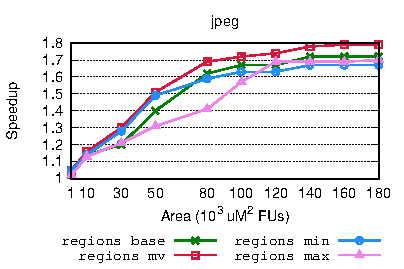
\includegraphics[width= 0.6 \linewidth]{figs/plot_O3CPU}
\hspace*{-1cm}
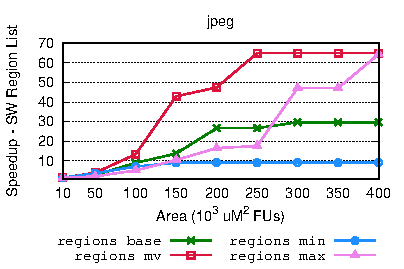
\includegraphics[width= 0.6 \linewidth]{figs/plot_O3CPU_SW_large}
\caption{Comparison of the speedup obtained by MuLTiVersioning to single 
versioning approaches on jpeg benchmark
varying the area constraint, using Aladdin and gem5 respectively, for HW and 
SW latency evaluation.
Top: Over the
total run time of the application. Bottom: Over the run time of the regions 
selected.  
% Four approaches are compared: The 
% min where the regions with least amount of area are selected, the base
% where the regions with median values of area are selected, the max where 
% only the maximum area regions can be selected and finally the \multi\
% approach where any version of the regions can be selected.
}
\label{fig:mlv_aladdin}
\end{figure*}

% \begin{figure*}[h]
% \centering
% \hspace*{-1cm}
% 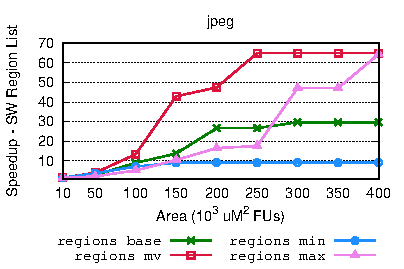
\includegraphics[width= 0.6 \linewidth]{figs/plot_O3CPU_SW_large}
% \caption{Comparison of speedup obtained on jpeg benchmark, over the
% SW time of the equivalent kernels (regions), varying the area constraint, using 
% Aladdin and gem5 for Speedup and Area evaluation.
% Four approaches are compared: The 
% min where the regions with least amount of area are selected, the base
% where the regions with median values of area are selected, the max where 
% only the maximum area regions can be selected and finally the \multi\
% approach where any version of the regions can be selected.
% }
% \label{fig:mlv_aladdin}
% \end{figure*}

The strength of the \multi\ approach and the benefit of having 
a variety of potential candidates to select from 
%for any equivalent computation, throughout the \jpeg\  application 
is demonstrated by the experimental outcome of the \jpeg\ application for different area constraints. 
In Figure \ref{fig:mlv_aladdin} (Top) for any given area point, the speedup obtained is higher than any other 
methodology. In Figure \ref{fig:mlv_aladdin} (Bottom) the distinction among the four different strategies, i.e., \multi\ compared to the three single-version methods, becomes more apparent. For a medium area point (200K  $uM^2$), the 
speedup achieved with \multi\ is 1.7x more than the second best, \emph{base} approach. For 
a large area constraint (400K $uM^2$) the \multi\ speedup is more than 2x compared to
\emph{base} and more than 6x compared to \emph{min}.\par

% In Figure \ref{fig:mlv_speed_aladdin} the same trend is depicted in the speedup of the whole application
% for the MuLTiVersioning methodology, where it constantly outperforms every other competitive method while
% reaching a maximum speedup of 1.8x over the entire jpeg application.\par



% \begin{figure}[h]
% \centering
% \hspace*{-1cm}
% 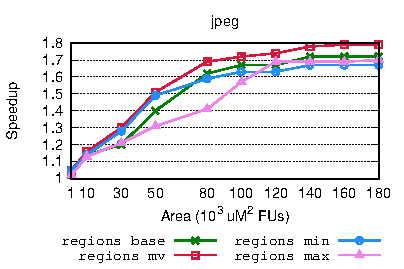
\includegraphics[width= 0.7 \linewidth]{Figs/plot_O3CPU}
% \caption{Comparison of speedup obtained on jpeg benchmark, 
% varying the area constraint, using 
% Aladdin and Gem5 for Speedup and Area evaluation.
% Four approaches are compared: The 
% min where the regions with least amount of area are selected, the base
% where the regions with median values of area are selected, the max where 
% only the maximum area regions can be selected and finally the MuLTiVersioning
% approach where any version of the regions can be selected.}
% \label{fig:mlv_speed_aladdin}
% \end{figure}


\section{Related Work}
\label{sec:rw}

Automatically identifying parts of computation to be
accelerated is often called, in literature, Instruction Set Extension
identification, or also HW/SW Partitioning. The distinction that is most 
relevant, for this research work, is the
\emph{scope} at which the suggested techniques perform identification: 
identifying accelerators or custom instructions at the \dataflow\ or
the \controlflow\ level.\par

%\subsection{Data Flow Level}
\emph{Data Flow Level}.
State-of-the-art methods have been
published in literature to automatically identify,
\emph{within a single basic block}, the subgraph of \dataflow\  
that maximize speedup when implemented in HW as a custom instruction
according to varying architectural constraints. A non-extensive list
include works \cite{YuSep04}, \cite{PozziJul06}, \cite{ChenFeb07},
\cite{ReddingtonAug09}, \cite{GiaquintaMar15} and \cite{MartiFeb12},
where the problem of identifying subgraphs under convexity, I/O
constraint, and/or area is tackled; in \cite{VermaOct07} and
\cite{PothineniJan07} the I/O constraint is relaxed, to be regained
via I/O serialization~\cite{PozziSep05}, \cite{VermaOct07},
\cite{AtasuApr07}, \cite{AhnJan13}. In \cite{CongFeb04} the focus of
the identification process is also on DFG nodes within single basic
blocks, and the constraints that are taken into account are a limited
number of read and write ports, and area.  The methodology proposed in
\cite{GaluzziOct06} is not limited by I/O in the selection process,
but clusters MAXMISOs \cite{AlippiMar99} in order to form MIMOs 
(Multiple Input Multiple Output instructions) that can be executed as 
a single instruction.\par

In none of the above pieces of research, though, the inclusion of the
\controlflow\ of the application is considered during the
identification process. The technique proposed in this chapter, 
instead, pushes 
identification \emph{beyond} the basic block level and identifies 
entire regions of the \CFG\ of the
application as candidates for acceleration. Compiler
transformations such as if-conversion and loop-unrolling can be, and
are, used by several of the techniques mentioned above in order to
enlarge the scope of within-basic-block identification, by enlarging 
basic blocks. Nevertheless, the scope remains limited to those
techniques and cannot include \emph{all} kinds of
\controlflow.\par

\emph{Control Flow Level.}
A smaller amount of research has looked into
identification within CFGs. In \cite{ZuluagaJul09} it is
proposed to implement CFG regions with multiple control exits as
accelerators. However, the presence of multiple control outputs
significantly complicates the processor-coprocessor interface, as
opposed to a single-entry single-exit approach. 
Another paper proposing HW/SW partitioning~\cite{BaleaniMay02}
presents a clustering methodology that operates on a control-data
network compiled from an Extended Finite State Machine (EFSM)
model. While it targets \controlflow\ to a certain extent, their
methodology is limited to applications that can be modeled using
EFSMs, therefore considering a much more limited scope than that of
generic Control Data Flow Graphs compiled from source code, as does 
the methodology proposed in this chapter.

Finally, the authors of a recent work \cite{AguilarJune16} consider
Single Entry Single Exit regions but their target is to identify
strictly parallelizable loop regions and offload them to an MPSoC
target platform. This approach is limited in
terms of excluding non-parallel regions from being potential
candidates to be accelerated, and also in terms of not being cost-efficient, in case a
designer needs to set a specific area constraint for the accelerators.

%\subsection{Compiler Transformations}
\emph{Compiler Transformations}.
Within compiler research, it is fairly 
common to identify CFG subgraphs for code
optimization reasons. For example, trace scheduling, superblock and
hyperblock scheduling~\cite{HankSep93}, identify regions
of the CFG in order to perform global code scheduling and
improve code generation. \emph{SESE} (Single Entry
Single Exit) regions have been proposed in~\cite{JohnsonJun94}, and
their identification was reimplemented in the LLVM framework in an 
analysis pass
called \emph{RegionInfo}, for the purpose of improving the
performance of code generation. For my SW analysis, the idea of
CFG region identification was borrowed from compiler research and was 
applied to automatically identify and select HW accelerators.

\emph{Application Specific Instruction set Processor (ASIP) architectures and design practices}.
HW Accelerators that are embedded
in an Application Specific Processor can be either developed as hardwired
Integrated Circuits (ICs), or mapped onto reprogrammable systems. In the
first scenario, examples of Application-Specific Integrated Circuit (ASIC) 
platforms exist, such as the
Tensilica Xtensa from Cadence \cite{TensilicaMar17} and the ARC
processor from Synopsys \cite{ArcDec16}. These tools can be extended with
accelerators and complex instructions. The CPUs can be configured
during the design process to maximize performance and efficiency,
without enduring the overhead of reconfiguration. An alternative, not 
as performing yet more flexible, is offered by FPGA-based
Systems-on-Chips (SoCs), such as the Arria10 family \cite{ArriaNov16} by Altera 
and the Zynq SoCs \cite{ZynqMar17} by Xilinx.\par

The instances mentioned above support the generation of HW
circuits, but do not provide implementation paths for differentiating the
execution between HW and SW. Conversely, High Level
Synthesis (HLS) tools allow designers to move parts of applications, 
written in C or C++, between processors and
accelerators. Research endeavors in this domain include LegUp
\cite{CanisSep13} and ROCCC \cite{GuoMar05}, while commercial
applications comprise the Vivado HLS \cite{VivadoHLSMar17} suite
from Xilinx (for FPGAs) and StratusHLS \cite{StratusHLSApr16} from
Cadence (for ASIC development).
However, these HLS frameworks place the responsibility of
partitioning a SW application on the application developer.\par

\section{Conclusions}
\label{sec:rs_conclusions}

The \rseeker\ framework, along with its %the \rseeker\ 
\multi\ extension, are methodologies that extend the \SoTA\ in the HW/SW co-design domain. They provide
efficient solutions to the problem of automatically deciding which parts of an application should
be synthesized to HW, under a given area budget. The accelerators identified by \rseeker\ 
consistently outperform the ones derived by data flow level algorithms and strictly function 
level candidates, across applications of widely different sizes and for varied area constraints.
As an example, \rseeker\ offers up to 4.5x speedup for the \mpeg\ benchmark compared to as SW
execution. This work was published in IEEE Transactions on Computer-Aided Design of Integrated 
Circuits and Systems (TCAD) journal \cite{ZacharopoulosApr19}.
The \multi\ approach extends the initial pool of candidates by introducing multiple optimized
versions of these candidates. Compared
to default HW accelerators configurations, \rseeker\ \multi\ offers enhanced speedup on the 
\jpeg\ application of up
% to 1.8 on the entire application and up 
to 65x speedup on the parts of the computation that 
are synthesized into HW compared to single-version approaches.
% meaning the computation time that is synthesized in HW excluding the time 
% that is left to SW.

% \begin{figure}
% \centering
% 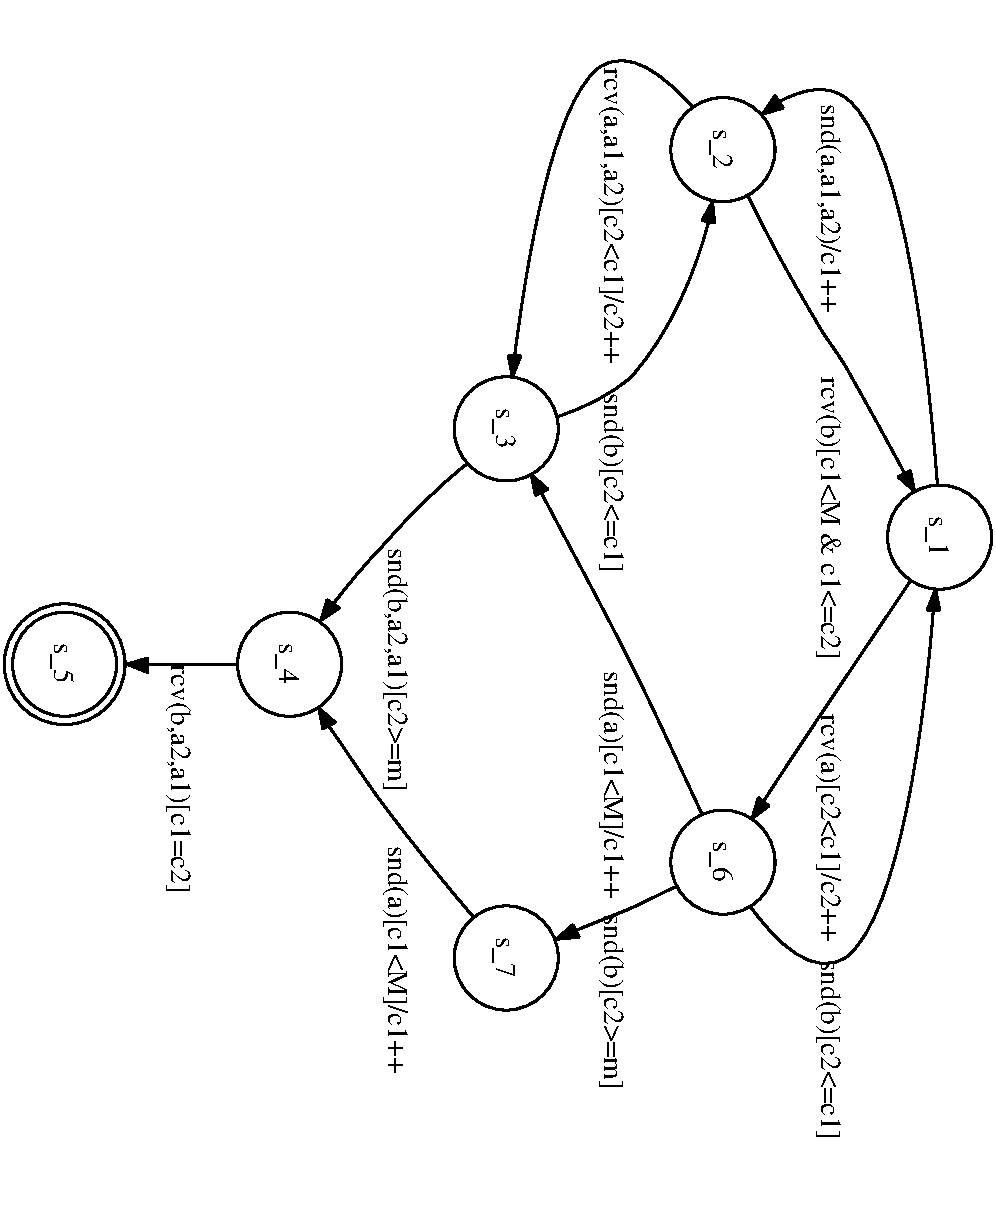
\includegraphics[scale=0.5,angle=90]{bounded_loop_automaton}
% \caption{\textsc{Automaton} for something or other. A caption can be rather
% long and \emph{should} then consist of complete sentences ended with a `.'}
% \end{figure}

% \section{The first \textsc{Section}}

% Here is some text with \textsc{SmallCaps} in normal font.

% \appendix %optional, use only if you have an appendix
% I removed mine a year ago.

%
%
%
%
%  
%     CHAPTER 2
%
%
%
%
%

\chapter{Automatic Optimizations for Accelerators}
% \vspace{-1cm}

Identifying good candidates for HW acceleration is the first step to realize heterogeneous
computing system designs that offer increased performance compared to a homogeneous system restricted
to general purpose SW CPU(s). However, a set of optimizations applied on HW accelerators can decrease 
even more the computation times, thus leading to an improved performance compared to default
non-optimized HW accelerator implementations. 
Modern \HLS\ (HLS) tools can apply such optimizations to 
HW accelerators and increase the performance of their implementations, as well as the overall performance 
of the entire heterogeneous system.
HLS tools such as Vivado HLS  \cite{VivadoHLSMar17}, however efficient, though, are far from 
optimal since they require a lot of manual decisions from the programmer's part when it comes to the
choice of {\em how} these accelerators can be synthesized.
Furthermore, the resolution of which optimizations may be applied to which HW accelerators can be a 
complex problem, as it depends heavily on each HW accelerator characteristics.\par

In order to bring automation one step forward in HW/SW co-design, and under the scope of this part of my 
research, I tackled the problem of automating the decision making process of which optimizations should be 
applied to candidates for HW acceleration within a certain context. 
These optimizations include memory management of the data consumed and produced by the HW accelerators, 
a set of optimizations targeted to loops (e.g. loop pipelining, loop unrolling, loop flattening etc), 
pipelining consecutive pieces of computation such as subsequent function calls or loop bodies of consecutive 
iterations and array optimizations, such as array partitioning in blocks of the same size. Among the various 
optimizations available, I have focused on two major categories: a) Data Reuse analysis and b) Loop Unrolling 
factor prediction. Both of these instances are explained in more detail in the following two sections.

\section{Data reuse Analysis}
\label{sec:dr}


\subsection{Motivation}

\begin{figure}[h]
\centering
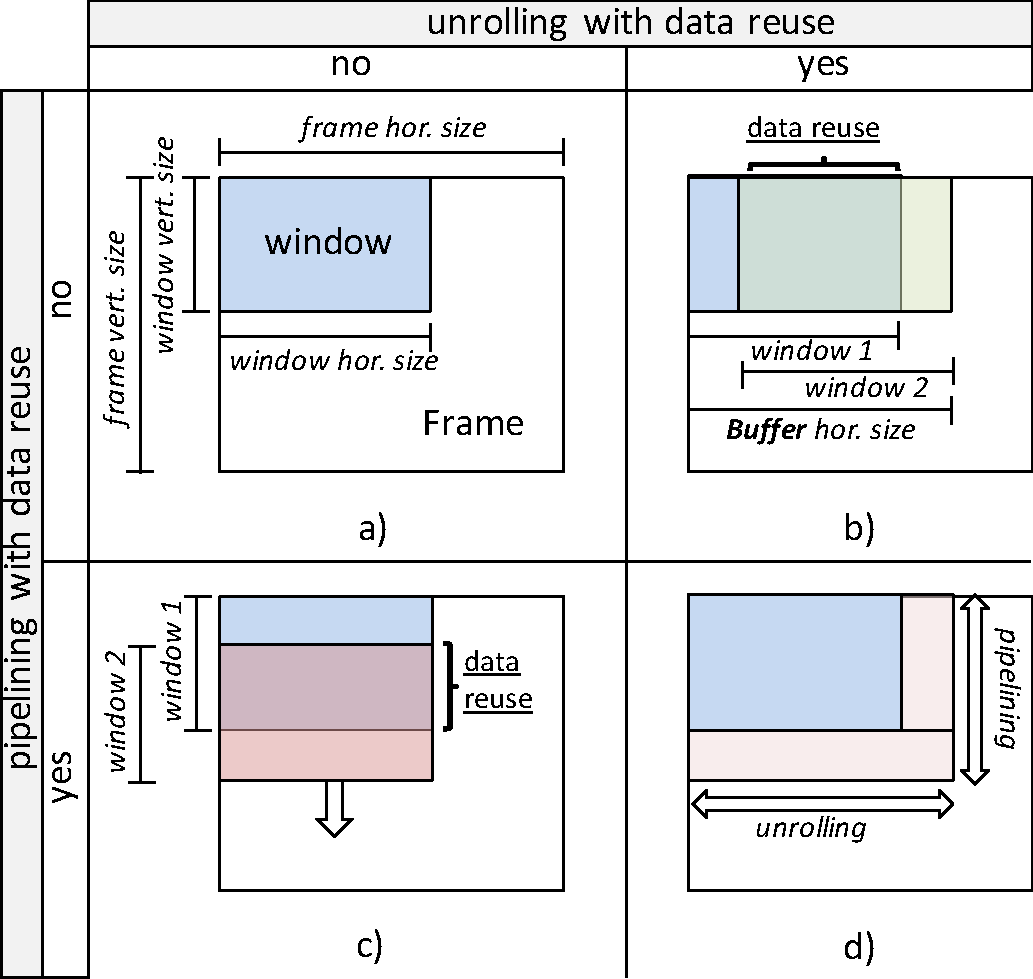
\includegraphics[width= .6 \linewidth]{figs/intro}
\vskip -.5em
\caption{At each iteration, sliding window applications process a
  subset of the input data (a).  The managed set of subsequent
  iterations present a high degree of overlap, both in the horizontal
  (b) and vertical (c) dimensions. The framework in \ref{sec:dr_meth} automatically
  leverages both, maximizing data reuse (d). }
  \vskip -1em
\label{fig:dr_intro}
\end{figure}

Loops are ideal candidates for acceleration. In almost every application, there is a
number of them that contain a large number of iterations and there is a sufficient 
amount of computation taking place in their bodies. In addition to that, there are 
nested loops which commonly show a high level of data reuse. An effective exploitation
of data reuse across consecutive iterations of loops can significantly lower the required
amount of data exchange between HW accelerators and the main memory, thus reducing the 
respective bandwidth to and from accelerators, and increasing their performance.\par

An example of such high
data reuse can be observed in sliding window applications, where there is typically
a window of accesses scanning a wider domain, such as a two-dimensional array. 
Given that the level and pattern of data reuse is known a priori, it is feasible 
to design specific memory structures, also known as memory buffers, attached to the 
HW accelerators. These memory buffers can exploit data reuse by keeping data locally 
and, hence, minimize the memory latency due to communication with the main memory.\par
 %while exploiting the computational potential of the accelerators.\par

Data reuse exploitation in \HLS\ (HLS) is still in premature stage.
State-of-the-art methods \cite{Vivado12} either rely on manually rewriting the source code, preceding HLS, 
or on source-to-source translation \cite{PouchetFeb13} \cite{SchmidJul15}, and are therefore 
poorly integrated in HLS tool-chains.\par
    
The methodology detailed in Subsection \ref{sec:dr_meth} attempts to bridge this gap. 
It presents a compiler-driven framework, based on the LLVM Polly~\cite{GrosserApr12} 
library, able to identify automatically data reuse potential in computational kernels in order
to guide the synthesis of complex HW accelerators.
As seen in Figure \ref{fig:dr_intro} these accelerators exploit timely unrolling and 
pipelining, by embedding a local storage holding elements which are re-used across iterations.\par
  
Sliding window applications, common in the image
processing field, are targeted for acceleration. In such domain, a transformation is 
applied to each element of a large two-dimensional input array (a frame) according to the
values in a smaller domain of accesses (a window). Large,
yet constrained, input/output links are considered as the main architectural
constraint in the design of this type of HW accelerators. Such arrangement is
usually supported by commercial application specific platforms, such as the Tensilica
Xtensa processor~\cite{TensilicaWeb}.

\subsection{Related Work}

In the domain of identifying automatically accelerators, research has 
so far focused mostly on accelerating data-flow~\cite{GiaquintaMar15} \cite{GutinFeb12}, 
not taking into equal account the potential for optimization by memory accesses. 
Exceptions are provided by papers \cite{BiswasMar06} \cite{ HaaBOct2014}
where the authors support the claim that accelerators with custom
storage can provide better speedup compared to the ones that
accelerate data-flow only. However, these papers focus on the
identification of the accelerators, and do not present a methodology 
to automatically identify the optimization potential, as well as
synthesize them accordingly.\par
In sliding window applications, there are research endeavors
both by academia and industry to exploit data reuse. The smart
buffers~\cite{GuoJun04} generated by the ROCCC
compiler~\cite{VillarrealMay10} allow for automatic detection of data
reuse opportunities, but cannot be interfaced 
with interconnects of varying width.
%
The methodology
described in \cite{MeeusMar14} employs reuse buffers spanning multiple
frame columns, which pose a significant area
overhead. Both \cite{GuoJun04} and \cite{MeeusMar14} are not able
to combine Hardware unrolling and pipelining, which are instead jointly
supported the methodology detailed in \ref{sec:dr_meth}. An alternative 
approach, described in
~\cite{DongMar07}, requires a great deal of \HW\ resources as well, as it 
requires the storage of large parts of a frame being processed inside the custom
hardware.  In~\cite{LeeserApr06}, the authors propose an analytical
method to gather microarchitectural parameters for sliding-window
applications on FPGAs. Their design however ultimately needs to be
manually implemented and hence the work neglects high level synthesis
aspects.\par
%
The commercial Vivado HLS tool requires
extensive manual rewrite of the source code, in order to instantiate
a reuse memory buffer. On the other hand, the approach presented 
% in \ref{sec:2_1_meth} 
here relies on automated code
analysis to derive the characteristics of the target application.\par 



\subsection{Methodology}
\label{sec:dr_meth}

In order to generate the custom-storage HW accelerators, a two-steps methodology is 
carried out. First the data reuse analysis of the application takes place and 
then the synthesis of the part of computation to be implemented in HW.
The first is performed with the utilization of compiler static source code analysis while
in the latter details regarding the hardware implementations are provided.
The phases of analysis and synthesis lead to the design and implementation of 
custom-storage accelerators that manage to minimize the latency due to data 
transfer between main memory and the HW accelerators.
% depicted in Figure \ref{fig:framework}, along with the evaluation
% procedure we follow. 



\begin{figure}[t]
\centering
%\hspace*{-2cm}
\vspace{-0.4cm}
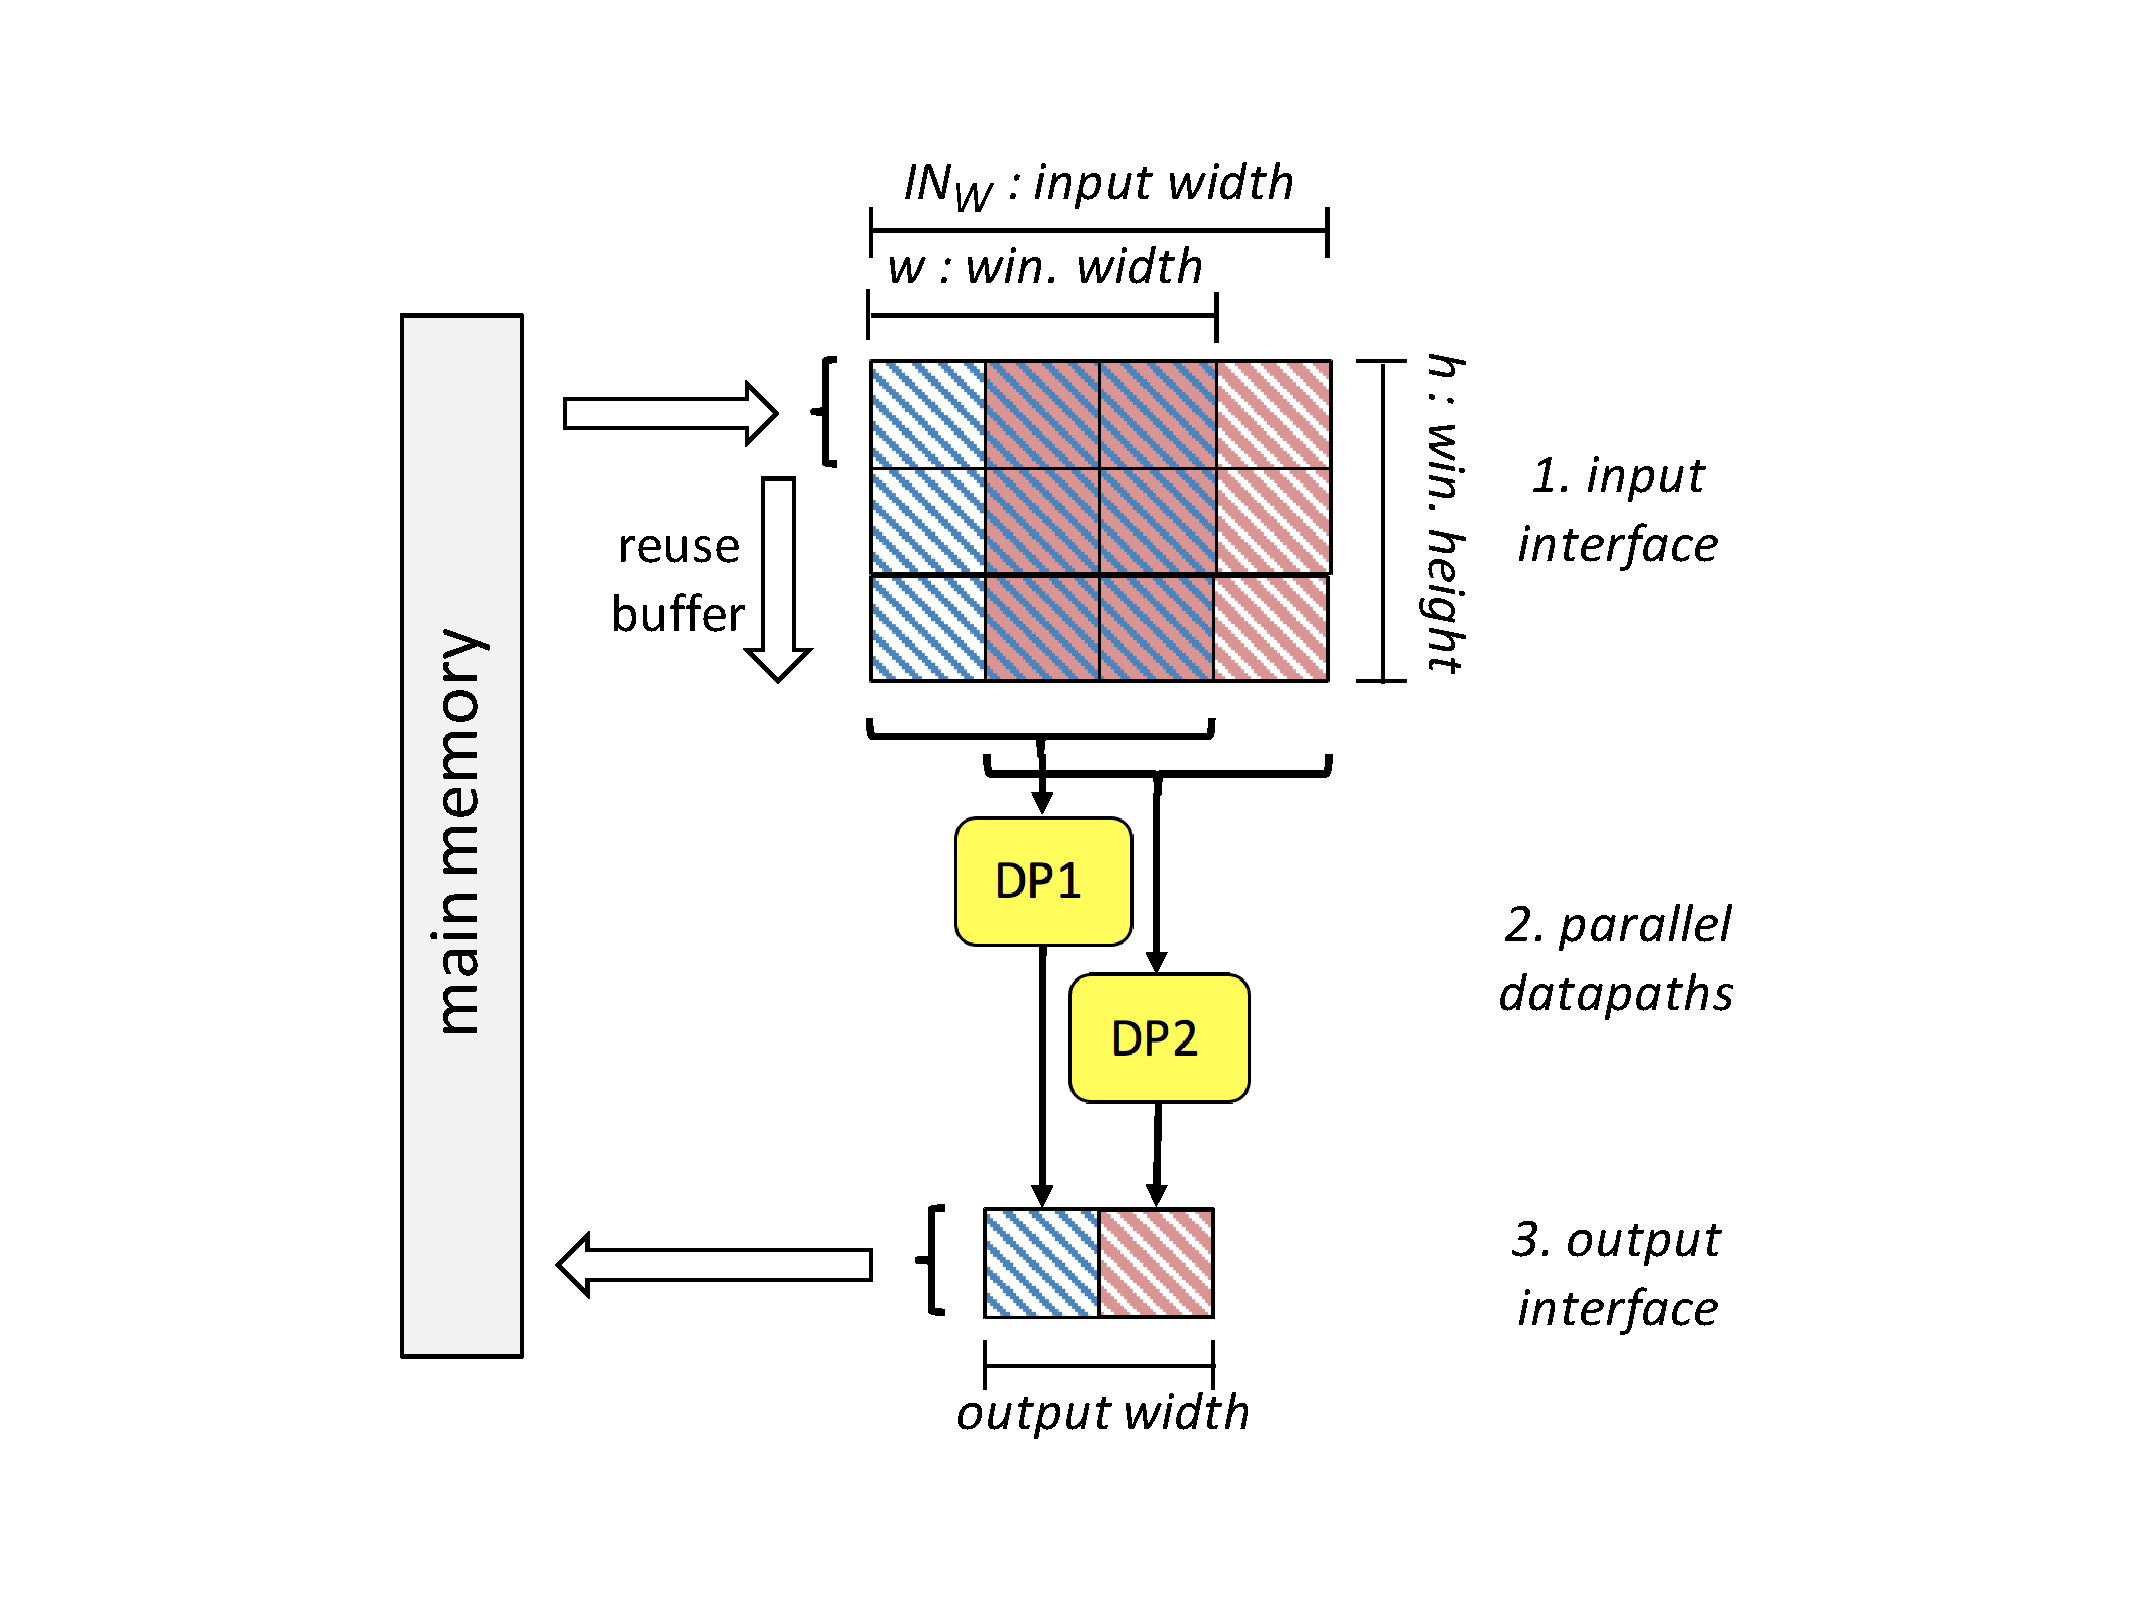
\includegraphics[width= .8 \linewidth]{figs/Data_Reuse}
\vspace*{-1cm}
\caption{Data Reuse of memory accesses (66.6\%) across consecutive iterations of a loop, in a sliding
window application.}
% \vspace*{-0.7cm}
% a figure\dots
% \caption{\textsc{Automaton} for something or other. A caption can be rather
% long and \emph{should} then consist of complete sentences ended with a `.'}
\label{fig:data_reuse}
\end{figure}


\subsubsection{Data Reuse Analysis}

In order to identify the level of data reuse that takes place throughout the execution of every
window application, there are three pieces of information that are vital: a) the size of the window, 
b) the stride and c) the frame size.
An example of data reuse, accounting for roughly 66\% the size of the window between consecutive 
iterations, can be seen in Figure \ref{fig:data_reuse}.
The window size is the access pattern
within the innermost body of the loop. The innermost and outermost
loop stride is the value of the induction variable increase for the innermost
and the outermost loop respectively. Finally, the frame size is
the iteration space within which the sliding window is moving. To extract this information 
I have developed an analysis pass, based on the LLVM Polly framework \cite{GrosserApr12}. 
Application-specific parameters are then considered in conjunction with architecture constraints 
(input/output width) to automate the synthesis of efficient HW accelerators.\par

\begin{algorithm}[t]
\begin{flushleft}
\textbf{Input:}  Application written in C/C++\\
\textbf{Output:} List of Identified SCoPs and their respective Frame, Window, Stride sizes/values.\\
\end{flushleft}
\begin{algorithmic}[1]
\Function{$RunOnRegion()$}{}
  \State\Call{$getAnalysis$}{ScopInfo}
  \State\Call{$scop=getScop()$}{}
  \State\Call{$RunOnScop$}{scop}
\EndFunction
\State
\Function{$RunOnScop$}{scop}
  \State\Call{$LI=getLoopInfo()$}{}
  \State\Call{$SE=getSE()$}{}
  \If {\Call{$L==OutermostLoop$}{}}
    \State\Call{$getTripCountFortLoop()$}{}
    \State\Call{$getStrideForLoop()$}{}
  \ElsIf  {\Call{$L==InnerMostLoop$}{}}
    \State\Call{$getReadMemoryAccesses()$}{}
    \State\Call{$ComputeDistancesForReadAccesses()$}{}
    \State\Call{$ComputeWindowSize()$}{}
  \EndIf
\EndFunction
\end{algorithmic}
\caption{LLVM Analysis Pass - SCoP Identification and 
Data Reuse Analysis}
\label{dr_Algo}
% \vspace{-0.2cm}
\end{algorithm}


The analysis pass, as seen in Algorithm  \ref{dr_Algo}, 
iterates over regions of the application 
functions and identifies Static Control Parts (SCoPs). The SCoPs are subgraphs of the control 
flow graph of a function 
where the flow of control is known statically. For each SCoP, loop and scalar evolution information
is collected from the body of the loop. \par

Loop information supports methods that can provide the 
loop depth, so as to identify the innermost loop. Scalar evolution information can be used to extract 
the loop trip count, which is the iteration space of each loop, and thus compute the frame size.
The stride value, both vertical and horizontal, is obtained by a function that was developed based
on existing methods of the Loop analysis LLVM pass.
%and receives as argument the Basic Block of the corresponding loop. 
Lastly, the read memory accesses of the innermost body of
the loop are identified by using \texttt{isl} functions, which
compute the
distance (or delta) of each of these read accesses with respect to the
first one. Given the access pattern, the window size is computed as the minimum 
enclosing rectangle. After having identified the necessary information, the implementation of a
local buffer that fits these needs can be carried out.\par

\subsubsection{Hardware Implementation}

The parameters retrieved with the analysis  pass (frame size, stride, horizontal and vertical window 
size) and the characteristics of the interconnect (input and output width) are employed to derive 
efficient HW accelerators implementation with local storage and data reuse.\par

As showcased in Figure \ref{fig:data_reuse}, accelerators implementations embed multiple 
combinatorial datapaths, each executing one iteration of the loop body of the target application.
The input interface embeds a local storage, whose horizontal size
corresponds to the available input data width of $IN_{W}$ data
elements, while its vertical size is equal to the vertical size
of the application window $h$. It is implemented as a $IN_{W} * h$
shift register, operating in the vertical (top-down) direction. During
execution, the first row of the shift register is filled with input
data in each clock cycle.  A subset of the elements stored in the
shift register is connected to each of the different datapaths
according to their managed sets, e.g.: the first one having inputs
corresponding to the buffer columns ranging from $0$ to $w - 1$ (the
horizontal size of the window) and the second one corresponding to the 
buffer columns ranging from $1$ to $w$.
Figure \ref{fig:data_reuse} illustrates such scheme for the simple case
of $IN_{W} = w+1$.\par

At the beginning of the execution, $h$ rows are stored in the shift register
before activating the datapaths logic. Afterwards, this activation is
performed for each new row, discarding the last (topmost) line and
storing a new one in the first (bottom) position of the shift
register. At the completion of a vertical slide of the window through
the frame, a new one is started, increasing the horizontal displacement 
of the buffer by $IN_{W} - w + 1$ elements.\par

Finally, since no reuse opportunities are present for outputs, 
the output interface simply concatenates the values generated by the datapaths, and
transfers them as a single and wide memory access. 

\begin{table}[t]
\begin{center}
\begin{tabular}{c|c|c|c}
%\hline
        &     \textbf{Pipelining}     &    \textbf{Unrolling}       &     \textbf{Parametric }   \\
                    & \textbf{data reuse}       &   \textbf{data reuse} &      \textbf{I/O width}          \\ \hline
\textbf{Our}             & Yes                & Yes                & Yes    \\ \hline
\textbf{Vivado}         & Manual            &  No                & Yes      \\ \hline
\textbf{ROCCC}          & Yes              & No                & No   \\ %\hline
\end{tabular}
\end{center}
\vskip -1em
\caption{Summary of the features of the accelerators generated by our framework, compared with state-of-the-art tools.}
\vskip -1.5em
\label{tab:tools}
\end{table}

\begin{table}[t]
\begin{center}
\vskip 1em
\begin{tabular}{c|c|c|c|c}
%\hline
        &     \textbf{Window}                 & \multicolumn{3}{c}{\textbf{Input width, \#DPs}}\\
\textbf{Benchmark}  &  \textbf{size}  &  \textbf{Conf.1} & \textbf{Conf.2} & \textbf{Conf.3}  \\ \hline
\textbf{SAD}             & 4x4                & 4, ~1   & ~8, ~5   & 16, ~13    \\ \hline
\textbf{Max. Filter}   & 8x8                 & 8, ~1   & 16, ~9  & 24, ~17    \\ \hline
\textbf{Sobel}           & 3x3                & 3, ~1   & ~8, ~6  & 16, ~14   \\ %\hline
\end{tabular}
\end{center}
\vskip -1em
\caption{Benchmarks characteristics and employed configurations. Conf.1 presents a 
  single datapath, while Conf.2  and Conf.3 have a moderate to large number of datapaths.
  Window sizes and input widths are expressed in bytes.}
  \vskip -1em
\label{tab:benchs}
\end{table}

\subsection{Experimental Results}
\label{sec:dr_exp}

The evaluation of this approach is carried out in three benchmarks of varying window sizes.
\texttt{Sobel} is an edge detection algorithm with an access pattern of a 3x3 window. \texttt{BlockSAD} 
is a kernel in \htsf and is used to detect the similarity among 4x4 blocks. Finally, 
\texttt{Maximum Filter} computes the brightest pixel among neighbors in 8x8 blocks. Three different 
configurations were considered, spanning from a singe datapath and minimum input width (Conf.1) 
to multiple datapaths and increased input width (Conf.2 and Conf.3) as seen in Figure \ref{fig:data_reuse}. 
Multiple datapaths translate to 
more parallel windows executing and, hence, increased demand in area resources.\par

The comparison of the approach introduced above is carried out against two state-of-the-art HLS 
tools: ROCCC and Vivado HLS. Vivado HLS is compared in two modes, one being the default (Vivado\_norew) 
and the other one after extensive manual rewrite of the source code (Vivado\_rew) in order to obtain 
increased data reuse.

\begin{figure}[h!]
\centering
\hspace*{-2cm}
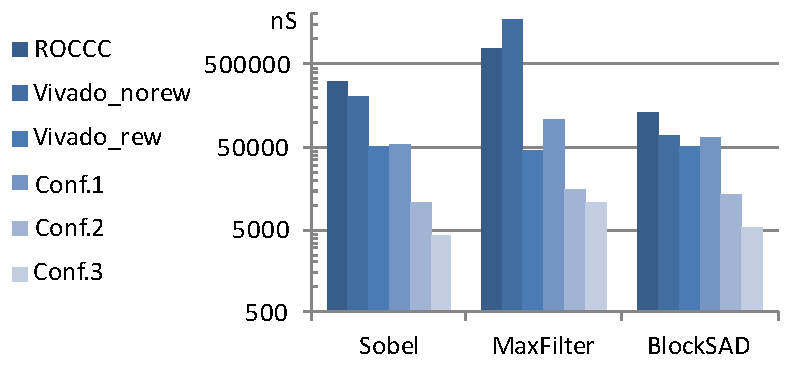
\includegraphics[width= .7 \linewidth]{figs/exec_time_fpga}
\caption{Execution time to process a 100x100 frame.}
\label{fig:exec_time_fpga}
\end{figure}

\begin{figure}[h!]
\centering
\hspace*{-1cm}
\vspace{1cm}
\vskip -1em 
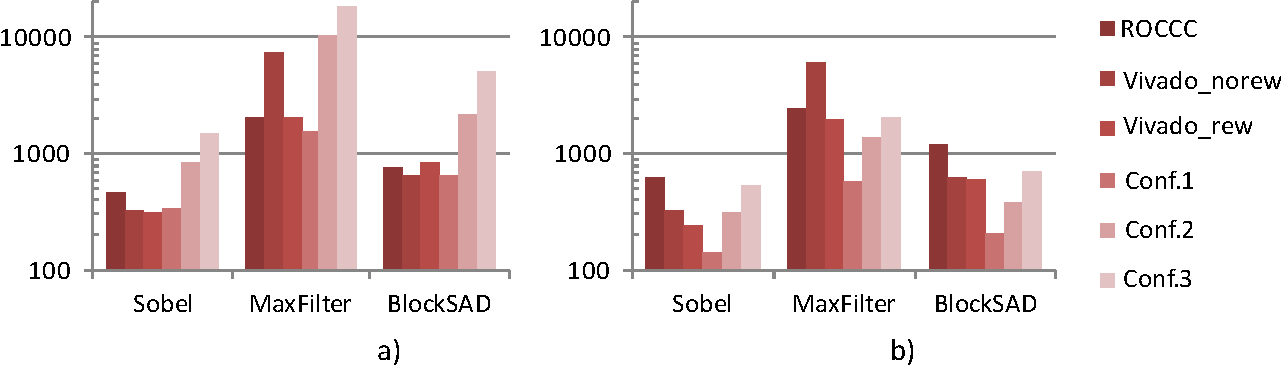
\includegraphics[width= 1 \textwidth]{figs/area_fpga}
\caption{Comparison of required resources for our generated systems and for baseline 
approaches: LUTs (a) and Flip-Flops (b).}
\label{fig:area_fpga}
\end{figure}

\textbf{Execution Time}. Execution time, as seen in Figure \ref{fig:exec_time_fpga}, 
is extracted from 
a targeted Xilinx Virtex7 FPGA platform. 
It can be observed that ROCCC systems have similar
performance with respect to Vivado\_norew ones. Conf.1 accelerators 
--- even though they do not require code modifications --- are as 
efficient as Vivado\_rew ones. Conf.2 and Conf. 3 that are
supported only by the framework presented in \ref{sec:dr_meth}, dramatically decrease
run-times, with an order-of-magnitude speed up on average between
Conf.1 and Conf.3. The other \SoTA\ tools \emph{fail to 
provide an equivalent solution with such low execution time}.\par

\textbf{Required resources}. Figure \ref{fig:area_fpga} reports the amount of area 
resources required by
ROCCC, Vivado HLS and our own generated accelerators.
Unsurprisingly, accelerators featuring a high number of datapaths (Conf.3) 
require more resources than single-datapaths approaches (Conf.1, Vivado). 
Nevertheless, the area increase in terms of Flip-Flops is comparable to 
the other to state-of-the-art tools, as the size of the buffer only is 
increased slightly to support a high degree of parallelism.
On the other hand, the results highlight that complex accelerators require 
an increased amount of combinatorial logic (LUTs), with respect to ROCCC 
and Vivado HLS.\par

 \begin{figure}[!t]
\centering
  \vskip 1em 
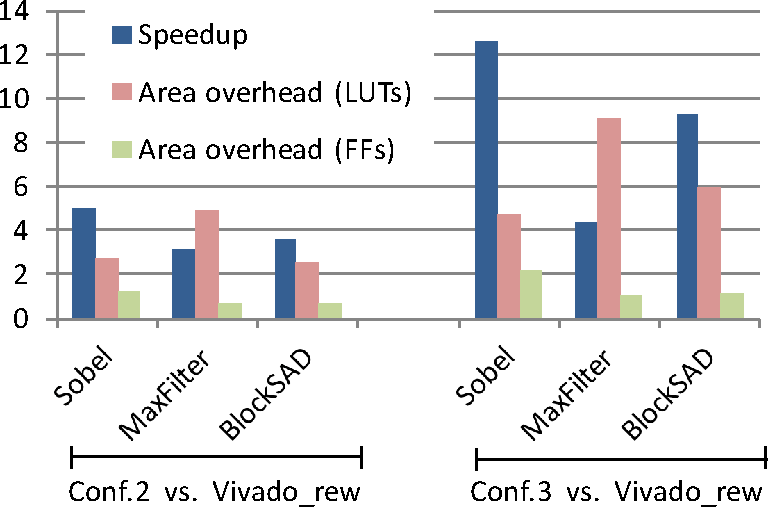
\includegraphics[width= .6\linewidth]{figs/comparison.pdf}
\caption{Comparison of multi-datapath  and optimised Vivado
  implementations.}
  \vskip -1em 
\label{fig:compar}
\end{figure}

 As illustrated in Figure \ref{fig:compar}, the speedup improvements
 due to parallel datapaths compare favourably with the area
 overheads: in the case of the BlockSAD benchmark, for example, 
 Conf.3, which embeds 13 parallel datapaths, requires 6x more LUTs
 with respect to the Vivado\_rew implementation, but at the same time
 results in a 9.2x speedup. Again, it is important to note that 
 \SoTA\ tools do not support unrolling with data reuse, 
 but stop at the level of speedup that can be achieved
 by single-datapath solutions.\par

The framework presented in \ref{sec:dr_meth} brings High-Level Synthesis
   one step closer to mimicking manual hardware-designer
   decisions. The Conf.3 accelerator for BlockSAD, presented above,
 is essentially the same as the one designed manually by Hameed et. al
 ~\cite{HameedOct11}, in a paper aimed at manually designing
 accelerators for the \htsf\ application. The authors have indeed chosen
 to invest area for as many as 16 BlockSAD datapaths in parallel, in
 order to 1) maximize speedup and reuse, and 2) exploit the high
 bandwidth present between processor and accelerator, in their Cadence
 Tensilica Xtensa processor~\cite{TensilicaWeb}. The present work
 mimics the rationale followed there, but is able to do so
 \emph{automatically}. HLS state of the art tools can automate some of
 the decisions taken by the framework presented in this section, but not 
 all --- in particular,
 they cannot automatically and jointly exploit unrolling and
 pipelining while considering reuse, and hence deliver the levels of
 speedup provided here.


% \vspace{-0.3cm}
\subsection{Conclusions}

It has been demonstrated that static source code analysis can be crucial, when it comes to 
automatically optimizing the synthesis of accelerators that are dedicated to 
sliding window applications. My SW analysis identifies data reuse, as well as data locality,
and subsequently allows to exploit these characteristics by making use of appropriate
memory buffers. The experimental results reveal an order-of-magnitude performance 
improvement with respect to \SoTA\ methodologies. This work was published in 
HiPEAC IMPACT 2017 Seventh International Workshop on Polyhedral Compilation Techniques 
\cite{ZacharopoulosJan17}. 



% SECTION 2.2
%
%
%

\section[Machine Learning Approach for Loop Unrolling\\ Factor Prediction]
{Machine Learning Approach for Loop Unrolling\\ Factor Prediction}
\label{sec:ml}

\subsection{Motivation}

\HLS\ tools, utilized to synthesize accelerators, require manual decisions to be made, so as 
to build efficient accelerators. These decisions regard the choice of high-level optimizations 
and transformations to be applied, therefore a good understanding of the SW parts to be 
accelerated is essential. Optimizations applied during synthesis can highly improve the performance 
achieved, as well as allocate less HW resources for a given computer architecture. Nonetheless, 
the selection of optimizations is a challenging task due to two main reasons. 
First, hardware synthesis is a time-consuming process, limiting in practice the amount of 
possible implementations that can be evaluated. Second, the effect of assigning different values to 
directives is difficult to foresee, due to low-level application characteristics.\par

Simulation tools such as Aladdin \cite{ShaoJul14} have been developed in order to rapidly 
estimate the performance and cost (area) of HLS-defined designs. Nonetheless, even when employing 
estimation tools, an exhaustive evaluation of all directives settings for each candidate accelerator 
in a heterogeneous system is still unfeasible beyond simple cases. Addressing
this challenge, a machine learning framework is proposed that is able to infer the proper 
implementation of an HLS design based on its characteristics, automatically derived from a source code 
analysis pass, based within the LLVM compiler framework \cite{LattnerMar04}.\par


Within the scope of this piece of research, the focus is placed on {\em loop unrolling}, an already 
well known optimization from the compiler domain, as well as the HW domain.
The loop unrolling optimization replicates the body of a loop a given number of times 
in order to expose parallelism, which especially in a HW implementation can lead to 
substantial speedup gains \cite{KurraApr07}. 
% On the other hand this might raise the need for more HW resources. 
This directive should nonetheless be applied sensibly, because it entails a high area cost for the 
duplicated logic; in addition, its ensuing benefits can be hampered by loop-carried dependencies 
and frequent memory accesses.\par

It is thus clear that there is a trade-off between execution time and the area budget that 
a computer architect has at hand, as well as the level of complexity and more potential 
side effects that need to be taken into consideration. Since HW realizations are targeted, 
the goal of this work is to reach a {\em sweet spot} between performance and HW resources.\par

Within the sphere of this research work, the following contributions are made.
First, a novel {\em \ML\ }
approach is introduced, based on Random Forest classification, 
instead of estimation-based models, to predict 
accurately the optimal loop unrolling factor of loops in applications to be synthesized
in HW. The use of this methodology can provide results with better prediction score
and in much less time, compared to the \SoTA.
Second, the whole process is fully automated, from the analysis of the input applications, 
using the LLVM compiler infrastructure \cite{LattnerMar04}, up to the training of the Random 
Forest Classifier. Finally, the trained \RF\ classifier can be used to generate accurate loop 
unrolling predictions for any given application -- a piece of information that can 
directly be used by an HLS tool such as Vivado HLS, in order to synthesize parts of these 
applications to HW.

\subsection{Related Work}

Research papers have explored the applicability of machine learning to apply
compiler optimizations. In \SW\ compilers, it has been
employed by Agakov et al. \cite{AgakovMar06} to speed up iterative compilation,
by Monsifrot et al. \cite{MonsifrotAug02} to produce compiler heuristics
and by Kulkarni et al. \cite{KulkarniOct12} to select the order in which optimization passes
should be performed. Stephenson et al. \cite{StephensonApr05} have made use of Supervised 
Classification, such as near neighbor (NN) classification 
and Support Vector Machines (SVM) methods, to produce accurate predictions in optimal unrolling 
factors.
In all above-mentioned research works the authors targeted \SW\ 
compilation; in Subsection \ref{sec:ml_exp}, a comparative performance evaluation of the 
framework presented in Subsection \ref{sec:ml_meth} to the methodology proposed by 
Stephenson et al. is carried out, showcasing the benefit of the choice of loop features and 
classification strategy in the HLS scenario.\par

Liu et al.  \cite{LiuJun13} used a \RF\
classification model in the context of HLS, extending the \ItRef\
framework proposed in \cite{MarianiApr12} \cite{PalermoNov09}
\cite{XydisMar13} and \cite{ZuluagaJun12}. They address a different
problem with respect to the one tackled in this section: that of retrieving the set of
Pareto-optimal implementations of a given design by navigating its
configuration space. A similar stance, addressing system-level design,
is illustrated by Ozisikyilmaz et al. \cite{OzisikyilmazJun08}.  As
opposed to these works, my aim is to perform a predictive assignment
of synthesis directives, based on a training performed on an independent
input set. This problem was also investigated by Kurra et
al. \cite{KurraApr07}. Contrary to their methodology, my methodology does not
depend on a detailed estimation delay model of the loop body so as to
predict loop unrolling factors in HLS instances.

\begin{figure}[h!]
\centering
% \hspace*{-2cm}
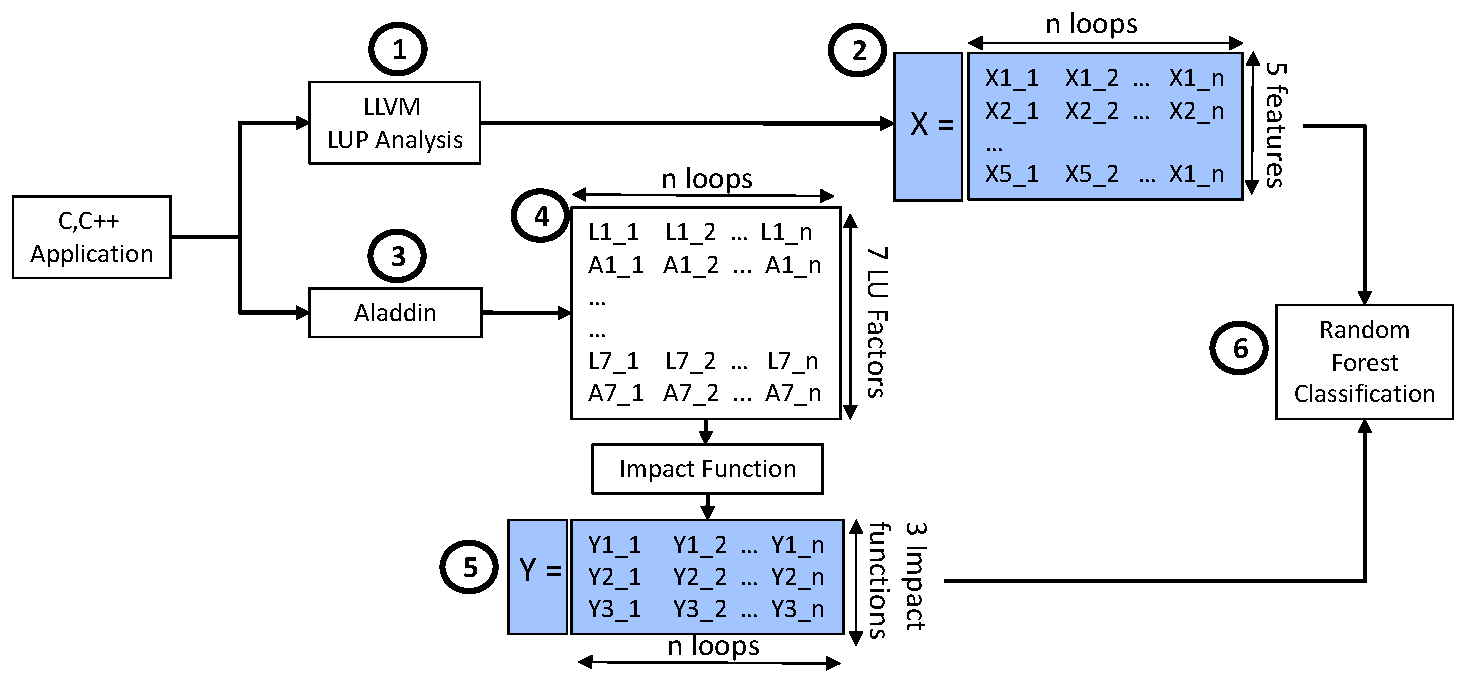
\includegraphics[width= 1 \linewidth]{figs/LUP_method}
\caption{Overview of the Loop Unrolling Prediction methodology.}
\label{fig:lup_method}
\end{figure}

\subsection{Methodology}
\label{sec:ml_meth}

In this section, first the employed objective function that determines the optimal loop 
unrolling factor is presented.
% , as well as the performance metrics considered to evaluate 
% the framework performance. 
Then, the LLVM analysis pass that was developed in order to 
automatically extract relevant loop features and the approach followed to retrieve the 
area and run-time performance of HLS designs is detailed. Lastly, the supervised learning 
classifier method is demonstrated, which, during the training phase, gathers the data from the 
previous steps to produce a loop unrolling predictor, and, during the test phases, assigns 
loop unrolling factors based on loop features.\par

\subsubsection{Optimal Loop Unrolling Factor -- Objective Function}

The {\em optimal loop unrolling factor} is defined as follows.
Given a defined set S of unrolling factors, e.g. S: <1, 2, 4, 8, 16, 32, 64>, there is one for every
loop that maximizes the \textbf {Impact (I)}, given by the following formula:

$$I(L,A)= \alpha  \cdot \dfrac{ (L_1 - L)} {L_1} + \beta \cdot \dfrac{ (A_1 - A)} {A_1},\ \alpha + \beta = 1$$

Where $L_1$ is the latency of the of the function containing a loop and being synthesized as HW 
accelerator, for Loop Unrolling Factor (LUF) that is equal to one, i.e., a fully rolled loop. $L$ 
is the latency of the HW accelerator for any possible LUF from the defined set.
Respectively, $A_1$ is the area resources requirements of the HW accelerator with LUF equal to one and 
$A$ the area for any possible LUF from the defined set.\par

Subsequently, the optimal LUF is defined as the one that maximizes the Impact function above. Note that, 
when $LUF = 1$, then $I(L,A)=0$ which corresponds to a baseline implementation. $I(L,A)$ may also 
be negative for suboptimal LUF choices (where unrolling might increase area without decreasing 
latency), but will always be $\ge 0$ for optimal unrolling factors.\par


For the evaluation presented in Subsection \ref{sec:ml_exp}
three different strategies were considered: a) Optimize for both latency and area ($\alpha = 
\beta = 0.5$). In this configuration a balance is maintained between decreasing the number of 
execution cycles and keeping low the usage of HW area resources in a given implementation.
b) Optimize for latency ($\alpha = 0.7, \beta = 0.3$). Minimizing latency is favored by this
approach, thus focusing on increasing the speedup of an application, and finally c) Optimize
for area ($\alpha = 0.3, \beta = 0.7$). This approach aims at decreasing the area budget of 
the implementation, therefore achieving an average speedup, but maintain low usage of HW 
area resources. All three configurations fulfill different architectural needs and explore 
realistic alternative scenarios.\par

% To evaluate the classification performance of a trained classifier, two different metrics were
% adopted. The \emph{Prediction Score} states the
% percentage of optimal (according to $I(L,A)$ ) LUFs that were correctly
% identified on the out-of-sample test set. The \emph{Average Error}
% instead measures the average distance between the indexes in $S$ of the
% correct and the predicted LUF.


\subsubsection{LLVM Analysis Pass -- Loop Features Extraction}

Loop features are automatically identified by an analysis pass (depicted as 
point 1 in Figure~\ref{fig:lup_method}) that was developed within the LLVM 
compiler infrastructure \cite{LattnerMar04}. Features are retrieved starting from
applications written in C or C++, operating on their Intermediate
Representation, provided by the LLVM front-end passes.\par  

My \textit{LLVM Loop Unrolling Prediction Analysis Pass} iterates over functions
of the applications and identifies loops. On each of them, it performs
loop, scalar evolution and dependence analysis to extract their
features, summarized in Table \ref{tab:X}: the critical path, the trip
count, the presence of loop carried dependencies and the required
memory accesses (load and stores).\par

% Table 1 and 2
%
%
\begin{table}[h]
  \centering

  \small\addtolength{\tabcolsep}{-3pt}
  \vspace{1em}
  \begin{tabular}{| l |} 
 \hline    
 \textbf{Features - X Vector}  \\ \hline
    \emph{Critical Path}      \\ \hline
   \emph{ Loop\ Trip\ Count} \\ \hline
   \emph{ Has\ Loop\ Carried\ Dependencies}     \\ \hline
   \emph{ \#\ Load\ Instructions}     \\ \hline
   \emph{ \#\ Store\ Instructions}      \\ \hline
  \end{tabular} 
    \caption{Features extracted by LLVM LU Analysis Pass.}
      \label{tab:X}
  
  
     \vspace{2em}
  

  \begin{tabular}{| l | l |} 
 \hline    
 \textbf{Features - X Vector 1} & \textbf{Features - X Vector 2}  \\ \hline
  \emph{\#\ Operands}        &\emph{\#\ Floating\ Point\ Operations}        \\ \hline
  \emph{Range\ Size}     &\emph{Loop\ Nest\ Level}   \\ \hline
    \emph{Critical\ Path}   &\emph{\#\ Operands}  \\ \hline
  \emph{\#\ Operations}      &\emph{\#\ Branches}   \\ \hline
  \emph{Loop\ Trip\ Count}&\emph{\#\ Memory\ Operations}   \\ \hline
  \end{tabular}
    \caption{Feature vectors selected by Stephenson et al. \cite{StephensonApr05}.}
      \label{tab:St_X1_X2}
\end{table}

The choice of features is based on the factors that influence the cost
and the achievable speedup of \HW\ unrolled loops: a loop with a
long critical path may be expensive to duplicate, while loop carried
dependencies and memory accesses may force a serialization of
execution irrespectively of the degree of unrolling. These
considerations lead us to consider a markedly different feature list
with respect to works focusing on software targets, such as the one of
Stephenson et al. (Table \ref{tab:St_X1_X2}).\par

\begin{algorithm}[t]
\begin{flushleft}
\textbf{Input:}  Application written in C, C++\\
\textbf{Output:} X (Feature Vector)\\
\end{flushleft}
\begin{algorithmic}[1]
\Function{\emph{RunOnFunction}} { }
  \For {\emph{BB\ in\ Function} }
    \If {{\emph{L=getLoopForBB}() } } {}
      \State{\emph{LoopUnrollingPredictionAnalysis}}{(BB,L)}
    \EndIf
  \EndFor
\EndFunction
\State
\Function{\emph{LoopUnrollingPredictionAnalysis}}{Basic Block BB, Loop L}
  \State{\emph{ LI=getLoopInfoAnalysis}()}
  \State{\emph{SE=getScalarEvolutionAnalysis()} } {}
  \State{\emph{DA=getDependenceAnalysis()}} {}
  \State{\emph{/*\ Gather\ Features\ for\ X\ Vector */} }
  \State{\emph{x1=getCriticalPath}}{(BB)}
  \State{\emph{x2=getTripCountForLoop}}{(L)}
  \State{\emph{x3=getLoopCarriedDependencies}}{(BB)}
  \State{\emph{x4=getNumberOfLoadInstructions}}{(BB)}
  \State{\emph{x5=getNumberOfStoreInstructions}}{(BB)}
\EndFunction
\end{algorithmic}
\caption{LLVM Analysis Pass - Loop Unrolling Prediction Analysis} 
\label{Algo_LLVM}

\end{algorithm}

\subsubsection{Latency and Area Estimation}
\label{sec:ml_la}

To establish a link between LUFs and performance/cost of
implementations, latency and area values must be extracted both for
the loops in the training set (in order to optimize the classifier)
and the ones in the test set (to measure its accuracy).%\par
Aladdin \cite{ShaoJul14} (point 3 in
Figure~\ref{fig:lup_method}), a pre-RTL power-performance simulator
for \HW\ accelerators was utilized in order to retrieve latency and area 
information. All functions in the considered benchmarks were
simulated by employing each feasible unrolling factor in the $S$ set 
defined above on every loop contained.  
Latency is reported by Aladdin in clock cycles,
while area is expressed in $\mu m^2$ in a $45nm$ technology. The
result is shown as point 4 in Figure~\ref{fig:lup_method}.
\par

The Impact ($I$) was computed afterwards for the different $\alpha$
and $\beta$ values, to retrieve the optimal loop unrolling factor for every loop
of a function, which is the index of the LUF that maximizes $I$. The
result is three vectors $\{Y1,Y2,Y3\}$ (point 5 in
Figure~\ref{fig:lup_method}) that contain the target values for the
classification algorithm. The $Y1$ vector includes the optimal loop
unrolling factor that balances the \HW\ implementation of the
accelerators in terms of low latency and low area. Values in the $Y2$
vector favors low-latency implementations, applying more aggressive
loop unrolling, whereas $Y3$ favors low-area ones.


\subsubsection{Random Forest Classification}


This information (X and Y vectors) extracted as described above are used 
as input to a Random Forest (RF) classifier (point 6 in
Figure~\ref{fig:lup_method}).
Supervised learning is performed by detecting the correlation between 
the input, the compiler extracted information, used as the X feature vector, 
and the output, which is the optimal loop unrolling factor for each loop.\par

\RF\ was used as the supervised learning model, which has been shown by Liu et al.
\cite{LiuJun13} to outperform alternatives such as Multilayer Neural Networks and \SVM\  
classification in the context of HLS design space exploration. \RF\ algorithms follow
a decision tree methodology, combining many weak classifiers to derive a strong one, allowing
the generation of low-complexity and robust classifiers.\par

\begin{algorithm}[t]
\begin{flushleft}
\textbf{Input:}  X and Y Vectors\\
\textbf{Output:} Trained Random Forest Classifier\\
\end{flushleft}
\begin{algorithmic}[1]
%\State{$NumberOfTrainingSessions=1000$}
\For {\emph{ i\ in\ NumberOfTrainingSessions} }
  \State{\emph{ X\_train, X\_test, Y\_train, Y\_test=train\_test\_split(X,Y)} }
  \State{\emph{ /*\ Training\ Phase\ */} }
  \State{\emph{ M=RandomForestLearningModel} }
  \State{\emph{ M.train(X\_train, Y\_train)} }
  \State{\emph{ /*\ Evaluation\ Phase\ */} }
  \State{\emph{ Pred=M.predict(X\_test)} }
  \State{\emph{ Error=abs(Pred-Y\_test)} }
  \State{\emph{ Score=M.score(X\_test-Y\_test)} }
\EndFor
\end{algorithmic}
\caption{Random Forest Classification -
 Training and Test} 
 \label{algo:RF}
\end{algorithm}

The algorithm employed, as presented in Algorithm \ref{algo:RF},
follows an approach similar to a \textit{k-fold cross validation}
strategy.  The whole data set ($X$ and $Y$ vectors, see points 2 and 5 
in Figure \ref{fig:lup_method}) is divided randomly
between a training set and a test set, where the training set is equal
to 80\% of the whole data set and the remaining 20\% is the test set.
Then, the \RF\ model is used for the training process on the training
set and out-of-sample predictions are carried out for each element of
the test set. After all predictions on the test set have been
computed, the prediction score and the average error (as defined in
Subsection \ref{sec:ml_exp}) are computed for the current training
session.\par

\subsection{Experimental Results}
\label{sec:ml_exp}

To evaluate the classification performance of a trained classifier, two different metrics were
adopted. The \emph{Prediction Score} states the
percentage of optimal (according to $I(L,A)$ ) LUFs that were correctly
identified on the out-of-sample test set. The \emph{Average Error}
instead measures the average distance between the indexes in $S$ of the
correct and the predicted LUF.\par

In order to comparatively evaluate the proposed methodology, combining \RF\ classification and
LLVM-based loop features extraction, benchmarks of different complexity were considered. Small 
and medium-sized ones are \adpcm, an audio encoding kernel, \stencil, an 
implementation of an iterative algorithm that updates array elements according to a given pattern, 
and \sha, a secure hash encryption method
used in the information security domain. \jpeg\ and \mpeg\ are instead larger benchmarks, which 
perform image and video compression, respectively.
Applications were drawn from the CHStone  \cite{HaraMay08} and the Scalable Heterogeneous 
Computing (SHOC) benchmark suites \cite{DanalisMar10}. In total, they comprise 87 different loops.\par

% The benchmarks used during the experimental phase are broadly used embedded applications from 
% the CHStone suite \cite{HaraMay08} and SHOC suite \cite{danalis2010scalable}.
%  \adpcm, \jpeg, \mpeg, \sha\ and \stencil.\par

Random Forest classification was implemented using the Scikit-learn suite \cite{PedregosaOct11}, 
that includes \SoTA\ implementations of \ML\ models in python. Scikit-learn was also employed to 
re-implement the two methods proposed by Stephenson et al. \cite{StephensonApr05}, that are consider 
as baselines.\par

Giving an initial proof of concept for the strategy proposed, Figure \ref{fig:dist} reports the 
difference between the indexes of the predicted optimal (according to impact value) loop unrolling 
factors and the ones retrieved with an exhaustive exploration, considering 18.000 out-of-sample 
predictions on all the benchmark loops. Results are highly concentrated on zero, 
indicating a high rate of correct predictions.\par

\begin{figure}[h]
\centering
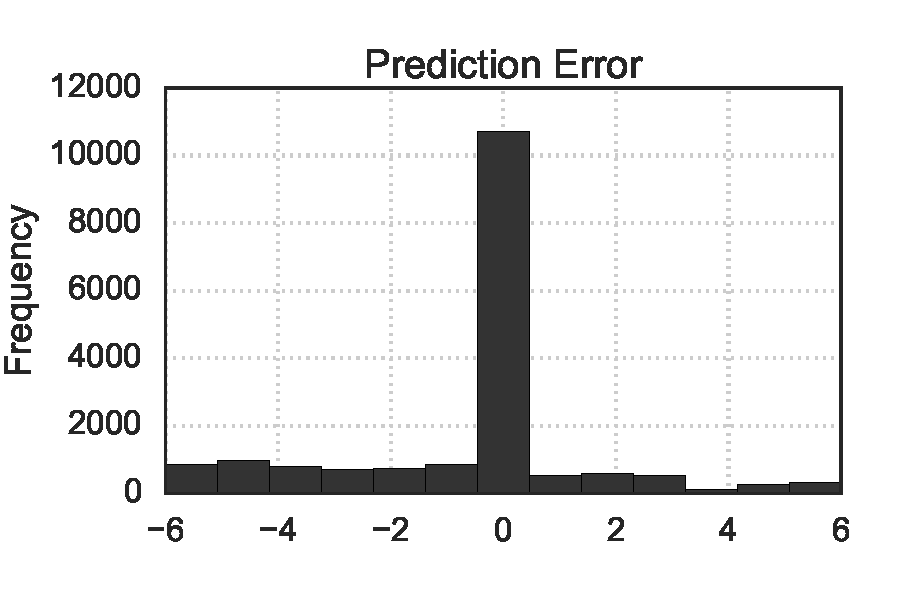
\includegraphics[width=.5\linewidth]{figs/prediction_errors}
\vspace{-1em}
\caption{Distribution of Loop Unrolling Factor Prediction Errors over 18.000 
out-of-sample predictions.}
\label{fig:dist}

\end{figure}

% During the experimental phase, state-of-the-art machine learning algorithms were used from the 
% Scikit-learn framework \cite{pedregosa2011scikit}.
% %  A Random Forest (RF) Classifier model is employed
% % to perform the classification. Results showcased a 60\% prediction absolute accuracy, meaning that the
% % predictions performed on the unknown subset of loops were correct 60\% of the time.
% As seen in Figure \ref{fig:mod_score} Random Forest (RF) is compared to Near Neighbor(NN) and
% Support Vector Machine (SVM) classifiers, and across different feature vectors. X as described
% above and X1,X2 by \cite{StephensonApr05}. The X1 and X2 features differ from the ones of X (e.g. X2: \# 
% Floating Point operations, loop nest level etc) as they target 
% SW execution. The suggested RF classifier and X feature vector 
% showcased a 60\% prediction absolute accuracy, meaning that the predictions performed on the unknown 
% subset of loops were correct 60\% of the time, outperforming every other state-of-the-art approach.

\subsubsection{Classification Models and Features}
\label{subsec:mode_feature}

The evaluation of the choice of features ($X$ vector in Table \ref{tab:X}) and training model \RF\ 
(RF), takes place against two \SoTA\ methodologies proposed by Stephenson et al. 
\cite{StephensonApr05}. The latter present different classification strategies: 
\SVM\ (SVM) and \NN\ (NN) and a different choice of investigated loop features, reported in 
Table \ref{tab:St_X1_X2}. Figure \ref{fig:mod_score} shows, for a choice of $\alpha = 0.5$, the 
prediction score and the average error of the nine strategies resulting from different feature 
vectors and classification strategies. Experimental results highlight that the presented framework 
($X$ feature vector and RF classification)
outperform other choices, reaching a prediction score above  60\% and an average error of
less than 1.4. Similar results were obtained for impact functions favoring area or latency
($Y2$ and $Y3$ vectors).



\begin{figure*}

\centering
%\hspace*{-2cm}
%\vspace{-0.4cm}
  \hspace*{-2cm}
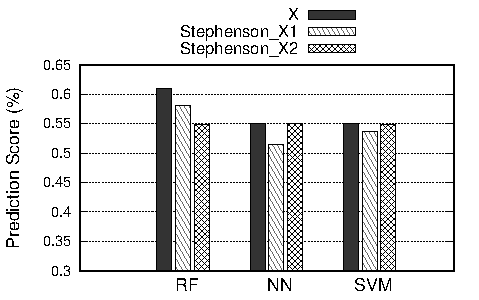
\includegraphics[width= .5 \linewidth]{figs/models_score}
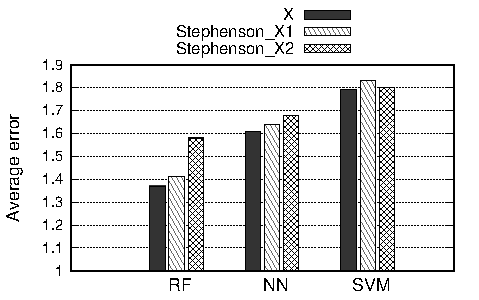
\includegraphics[width= .5 \linewidth]{figs/models_error}
% \vspace*{-0.2cm}
\hspace*{-2cm}
\vspace*{-0.2cm}
\caption{Left: Comparison of the Prediction Score across Random Forest, Nearest Neighbor, Support Vector Machines models 
and the respective feature selection: X vector, Stephenson et al. X1 and X2 vectors \cite{StephensonApr05}.
Right: Features extracted by my LLVM Loop Unrolling Analysis Pass.}
\label{fig:mod_score}
% \vspace*{-0.7cm}
\end{figure*}




\subsubsection{Iterative Refinement}

In the second round of experiments, the comparison of the proposed method was carried out against an 
\ItRef\ approach, used in \cite{MarianiApr12} \cite{PalermoNov09} \cite{XydisMar13} \cite{ZuluagaJun12}. 
\ItRef\ uses part of the training data set
to obtain a first version of the classifier, whose performance is then improved by using a second,
disjoint set of input and outputs.\par

For this evaluation, three different settings of Y target vectors $\{Y1,Y2,Y3\}$ were considered, as 
described in Subsection \ref{sec:ml_la}. The employed data,
the features ($X$ vector) and the training model (\RF) were the same both for Algorithm \ref{algo:RF} 
and the one using \ItRef. For \ItRef, 75\% of the training set is allocated for the 
initial training phase, and the remaining 25\% for the refinement phase.

\begin{figure*}
\centering
%\hspace*{-2cm}
%\vspace{-0.4cm}
  \hspace*{-2cm}
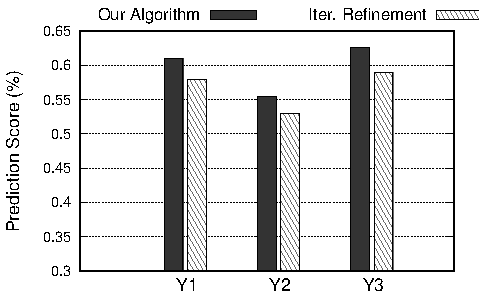
\includegraphics[width= .5 \linewidth]{figs/iter_ref_score}
\includegraphics[width= .5 \linewidth]{figs/iter_ref_error}
% \vspace*{-0.2cm}
\hspace*{-2cm}
\vspace*{-0.2cm}
\caption{Left: Comparison of the Prediction Score across Random Forest, Nearest Neighbor, Support Vector Machines models 
and the respective feature selection: X vector, Stephenson et al. X1 and X2 vectors \cite{StephensonApr05}.
Right: Features extracted by my LLVM Loop Unrolling Analysis Pass.}
\label{fig:iter_ref_score}
% \vspace*{-0.7cm}
\end{figure*}

The prediction score, as seen in Figure \ref{fig:iter_ref_score}, ranges from 53\% to 63\% across the three 
$Y$ vectors. Nevertheless, our methodology consistently outperforms the \ItRef\ approach, while achieving 
the highest prediction score (63\%) for the setting that favors low area resources ($Y3$). A similar
observation can be made for the average error values, where the suggested approach keeps a lower 
average error for all predictions, across all vectors, with the one related to the $Y3$ vector 
being the lowest (1.32).\par

Figure \ref{fig:speed_ir} reports the speedup, area and impact metrics of HLS designs
optimized with our predictive method, comparing them to an \ItRef\ approach and to results obtained
from an exhaustive exploration. 
The graphs correspond to an impact function with $\alpha = 0.9$ 
(similar results were obtained for other $\alpha$ values). Two considerations can be drawn from the reported data: first, in most cases the methodology presented in the section
closely tracks the user-defined trade-off between area and latency. In this respect,
\texttt{jpeg-huff} and \texttt{stencil-stencil} are outliers, since their loop structure is quite complex,
making their optimization challenging to automate. Second,
the impact achieved by our approach is equal or higher (by 66\% in the case of \mpeg) than the
impact attained by \ItRef. On average, our methodology obtains 86\%
of the speedup achieved by the optimal factor retrieved with
a costly exhaustive exploration (90\% for $\alpha = 0.5$  and 92\% for
$\alpha = 0.1$).

% Speedup/Impact - IterRef 
%
%
\begin{figure*}[h!]
\centering
\hspace*{-1cm}
\includegraphics[width=1.1\textwidth]{figs/iter_ref_abs_speed_c90.pdf}\\
\vspace{-1em}
\hspace*{-1cm}
\includegraphics[width=1.1\textwidth]{figs/iter_ref_abs_area_c90.pdf}\\
\vspace{-1em}
\hspace*{-1cm}
\includegraphics[width=1.1\textwidth]{figs/iter_ref_abs_impact_c90.pdf}
\vspace{-2em}
\caption{Comparison of the Speedup, Area and Impact achieved for every function by our 
Algorithm and by an \ItRef\ approach \cite{MarianiApr12} \cite{PalermoNov09}
\cite{XydisMar13} \cite{ZuluagaJun12}, compared to the optimal solutions derived from
exhaustive explorations. Speedup and Area numbers are normalized with respect to
fully rolled configurations.}
\vspace{2em}
\label{fig:speed_ir}
\end{figure*}


\subsubsection{Convergence Time Comparison}


Besides retrieving high-quality LUF predictions, the framework presented here also requires
a lower computational effort with respect to other methods.
In this regard, experimental evidence is shown in Figure \ref{fig:time},
reporting the time required for training and testing, comparing
different classification strategies, feature vectors and impact functions.\par

As expected, the choice of employed features, as well as the relative relevance of
area and latency, does not tangibly impact the computing time. On the other hand,
the type of employed classifier has a noticeable effect, with Random Forest
being slower to converge than NN and SVM. Nonetheless, only 14 seconds were
required by our approach. The difference between the \ItRef\ 
approach and our methodology, though, is even
more significant, as the the former requires almost four times more than our 
methodology to converge.\par

It is worthwhile to mention that all these approaches 
 require orders of magnitude less convergence time with respect to exhaustive explorations, 
 whose runtime may range from minutes (for estimation tools like Aladdin \cite{ShaoJul14})
 to hours (for synthesis frameworks such as Vivado HLS \cite{VivadoHLSMar17}).


% Time Comparison
%
%
\begin{figure}[t]
\centering
\subfigure{
  \hspace*{-1cm}
\includegraphics[width=0.5\textwidth]{figs/models_time.pdf}
}
 % \vspace{1em}
\subfigure{
\includegraphics[width=0.5\textwidth]{figs/iter_ref_time.pdf}
}
\vspace{-1em}
\caption{Left: time required to converge for \SoTA\ \ML\ models with  
our X feature vector and
Stephenson et al. X1 and X2 vectors \cite{StephensonApr05}. Right: convergence time
of our algorithm
and \ItRef\ across all three Y vectors. 
}
\vspace{-1em}
\label{fig:time}
\end{figure}

\subsection{Conclusions}

A novel methodology based on LLVM analysis and Random Forest classification that performs loop unrolling 
factor prediction for HLS designs was performed. This approach achieves better prediction score 
in comparison to state-of-the-art Machine Learning methods. Experimental evidence showcases that, 
by carrying out accurate predictions of loop unrolling factors, high performance accelerator 
implementations can be realized, while avoiding time-consuming exhaustive explorations. This work was 
published in the 2018 International Conference on High Performance Computing \& Simulation (HPCS) 
\cite{ZacharopoulosJul18}.


%
%
%
%
%  
%     CHAPTER 3
%
%
%
%
%


\chapter[Identification and Selection of System Aware Accelerators]
{Identification and Selection of \\ System Aware Accelerators}
% {System Aware Accelerators Identification --- Speedup and Energy Efficiency}

In this chapter of the dissertation the notion of automatic selection of HW accelerators is extended
by increasing the scope of the candidates for acceleration, in order to target demanding platforms 
with a complex memory hierarchy, such as a Xilinx Zynq Ultrascale+ PSoC board.
The acceleration of large and complex
applications, such as the H.264 decoder \cite{LiuFeb16}, necessitates the need to take into account the 
underlying system where the specialized accelerators are hosted. 
%and the latency due to communication between the main memory and the accelerators. 
The granularity of the candidates for acceleration is 
expanded to that of a subgraph of the entire call graph of an application and subsequently the need to 
accommodate for the communication overhead between main memory and the HW accelerators emerges.
% to that of a subgraph of the entire function call graph of an application.
%  Moreover, the underlying system is taken into account where the specialized 
% accelerators are hosted. 
The knowledge
of the characteristics of the system that is targeted can be critical for the choice of the HW accelerators
to be implemented. The memory system of a platform for instance can vastly affect the latency due to data
exchange between the main memory of the system and the HW accelerators.\par

\aseeker, an LLVM-based tool-chain, is presented as a framework that performs automatic identification 
and selection of HW accelerators targeted to a specific \SoC\ (SoC).
\aseeker\ performs thorough analysis of applications source code and estimates memory latency along with 
computational latency of candidates for acceleration. \aseeker\ selects accelerators that can minimize the
overall latency of an application and can offer increased speedup compared to %\SoTA\ 
profiling-only based approaches that mimic the manual decisions of a designer.\par
% The granularity of the candidates for acceleration 
% is expanded to that of a subgraph of the entire call graph of an application to accommodate for the 
% communication overhead between main memory and the HW accelerators.
In addition to accelerators targeting speedup, an extension of this methodology can focus on 
energy-saving 
heterogeneous designs. \eseeker\ extends the latency estimation of the previous framework and accounts for 
power estimation of hardware and software in order to target energy efficient HW accelerators. \eseeker\ 
performs identification and selection of accelerators that can offer substantial energy benefits to a 
heterogeneous computing system compared to a powerful, yet power-hungry, software processor and against  methodologies based solely on profiling information.
% \textbf{NOTE:} Write for EnergySeeker.

% AccelSSeeker 3.1
% 
%
%
%
%

\section{\aseeker: Accelerators for Speedup}
\label{sec:accel}

\subsection{Motivation}

System-level design, and heterogeneous computing as a whole, is witnessing a breakthrough. 
Emerging best practices based on High Level Synthesis (HLS) allow unprecedented productivity levels. 
HLS dramatically shortens development cycles by employing C/C++ descriptions as entry points 
for the development of both \SW\ (SW) and \HW\ (HW), greatly facilitating the task of migrating 
functionalities between the two.\par

However, the design of heterogeneous systems comprising SW processors and HW accelerators is 
still a demanding endeavor, during which key decisions are left solely to manual effort and 
designer expertise \cite{CacciottiSep18} \cite{NouriJun17}. Furthermore, the long time required 
for HW synthesis, coupled with the huge space of alternative implementations exposed by real-world 
applications, limits in practice the number of accelerator choices that can be considered manually 
by a designer before HW/SW partitioning is settled.\par

Addressing these issues, performance estimators have been proposed
that, while not providing working hardware implementations, can gauge
the characteristics of different accelerator implementation
alternatives  \cite{ShaoOct16} \cite{KathailFeb16}.  
Nonetheless, these tools can only evaluate one choice of accelerated
function at once. Hence, when using them, the evaluation of each
potentially viable HW/SW partitioning alternative requires
distinct experimental runs, a time-consuming task for large-sized
target applications.\par

In order to limit the entailed designer effort, it is therefore crucial to identify the set of viable 
acceleration options quickly, and also early in the design process, before performing later and more 
detailed estimations. This key step is currently poorly supported by design automation tools. Indeed, 
\SoTA\ early partitioning strategies are solely based on profiling information \cite{XilinxESTRef18} 
\cite{LattnerMar04} which, as was also shown by the authors of \cite{SyrowikJun18}, may often be 
misleading.\par

To fill this gap and offer an efficient solution to the problem stated above, \aseeker\ is presented. 
\aseeker\ offers a methodology to identify and select the suitable acceleration candidates in an
application, from its software source code. Being implemented within the LLVM \cite{LattnerMar04} compiler 
infrastructure, it first models an estimation of the cost (required resources) and merit (potential speedup) 
of all candidate accelerators in a single, quick pass, and then selects the set that maximizes the estimated 
speedup, while not exceeding a resource target. The use of \aseeker\ can therefore guide Integrated Circuit 
architects in the early design phases, highlighting which segments of a computing flow should be
targeted with HLS, and hence where to focus the process of applying optimizations to.\par

On the other hand, it indicates which parts are not likely to yield tangible benefits if realized in HW --- either 
because they present a low computational footprint, or because their characteristics hamper their potential for HW 
acceleration, e.g. they require an excessive amount of data transfers while performing limited computations.\par

The approach of \aseeker\ is markedly different from that of performance estimators, as the most promising 
candidates are identified in a single, high-level exploration, reducing the scope of further, and more detailed, 
estimations. It also differs from approaches based solely on profiling information, as profilers do not offer a 
measure of costs and run-times of HW implementations. Furthermore, they do not account for invocation overheads -- 
potentially leading to the selection of frequently called, but small, candidates. Finally, the transfer of data is an 
important factor that \SoTA\ profilers do not take into account -- hence potentially suggesting candidates 
requiring an excessive amount of communication, that in turn can significantly weaken any potential performance 
gained. \aseeker, instead, takes into account both the communication overhead and a number of the characteristics of the 
platform that are required in order to generate an estimation model which leads
to high-performance HW accelerators choices.

\subsection{Related Work}

High Level Synthesis tools have considerably matured in recent years \cite{MeeusSep12}. Nowadays, available 
commercial tools (e.g.: Xilinx Vivado HLS \cite{VivadoHLSMar17}, Cadence Stratus HLS \cite{StratusHLSApr16}), 
as well as academic alternatives (e.g.: Legup \cite{CanisSep13}, Bambu \cite{PilatoMar12}) support the design 
of very large accelerators from C/C++ code. They reach performance levels comparable to hand-crafted 
implementations specified in low-level Hardware Description Languages (HDL) such as VHDL or Verilog 
\cite{LiuFeb16}.\par

\begin{figure}[!t]
  
  \centering
  \includegraphics[width= .8 \linewidth]{figs/soa_evolution.pdf}
    \vskip -.5em
  \caption{Evolution of the SoA in automatic selection of custom
          instructions/accelerators: (a) from data-flow level
          \cite{PozziJul06} \cite{GiaquintaMar15}, (b) to control-flow
          level (\rseeker\ in Chapter 1) \cite{ZacharopoulosApr19} \cite{OppermannJul16}, (c)
          to function-call graph level (\aseeker\ in this chapter).}
  \label{fig:soa-evolution}
  \vskip -1em
\end{figure}

Nonetheless, the automated selection of the application parts most
amenable to HW acceleration is still an open research topic.
Selection approaches based on synthesis results \cite{CanisSep13b}
scale poorly to complex applications, as these are only available late
in the design process.  Estimation frameworks offer a detailed
analysis on the performance and resource requirements of a
HW-accelerated system while avoiding full synthesis runs, either
by interfacing software and HW simulators (e.g., gem5
\cite{BinkertFeb11} and Aladdin \cite{ShaoJul14} in \cite{ShaoOct16}),
or by adopting a hybrid stance, in which HW execution times are
estimated, while software ones are measured on a target platform (as
in Xilinx SdSoC \cite{KathailFeb16}). However, in both cases,
estimations are performed \emph{after} the partitioning of HW
and software, which is left to a trial-and-error basis.
A methodical solution for partitioning is instead proposed in this
chapter.\par

The downside of poor partitioning choices, and consequently the
importance of automated tools such \aseeker\ that guide the selection
of high-quality accelerator sets, is even more prominent when
considering the high effort required to optimize the implementation of
HLS-defined accelerators. Design optimization entails the
specification of multiple directives to steer designs towards the
desired area-performance trade-off. The link between directives and
the performance of implementations is not straightforward, hence
requiring the evaluation of multiple alternatives to reach the
intended results, as exemplified in \cite{SchaferJun12}
\cite{ZuluagaJun12} \cite{FerrettiJan18} \cite{LiuJun13}. It is
therefore key to focus up-front this optimization effort only on those
candidate accelerators which can lead, from an application
perspective, to tangible speedups.\par

To this end, the approach introduced here is inspired by previous works 
on automatic
identification of instruction set extensions. Most techniques in this
field target customizable processors augmented with
application-specific functional units, within the processor pipelines.
Hence, these techniques usually constrain their search to the scope of
single basic blocks \cite{PozziJul06} \cite{GiaquintaMar15}, as
depicted in Figure~\ref{fig:soa-evolution}a. In Chapter 1, with the 
presentation of the \rseeker\ framework, and in \cite{OppermannJul16} 
there was instead a focus on the identification of larger code segments, including
control-flow structures belonging to single functions (depicted in
Figure~\ref{fig:soa-evolution}b).  However, such scope still falls
short of the one employed in HLS tools, which are devoted to the
implementation of dedicated accelerators interfaced on a system bus
\cite{CotaJun15}. In this setting, the cost of data movement becomes
so prominent that even control-flow structures inside functions fail
to deliver performance. Suitable accelerator candidates must then
encompass entire functions, including in turn all functions called
within their call tree. \aseeker\ considers this same granularity
(Figure~\ref{fig:soa-evolution}c), advancing the \SoTA\ in
automatic accelerators identification.

% \subsection{Methodology}

The methodology of \aseeker, as depicted in Figure \ref{fig:flow}, is presented in 
more detail in the following subsections.  
First, the definition of a candidate for acceleration is given. Then the selection 
process of a subset of candidates, among a pool of such candidates, to be implemented in 
hardware is described (A and C in the figure). Finally, the approach employed to estimate 
the candidates performance (Merit) and resource requirements (Cost) (B in the figure) is presented.

\begin{figure}[!t]
  \centering
  \includegraphics[width= 0.7\linewidth]{figs/flow.pdf}
      % \vskip -0.5em
  \caption{The phases of the \aseeker\ approach. A) Candidates
          for acceleration are identified, from source code
          analysis. B) Given an estimation of merit and cost for each
          candidate, and C) given a maximum available cost, \aseeker\
          performs selection of a subset of such candidates.}
  \label{fig:flow}
      % \vskip -0.5em
\end{figure}

\subsection{Candidate Identification}
\label{subsec:identification}

In order to discover which parts of an application can be most
profitably accelerated in hardware, the investigation of its function-call
graph takes place, i.e., a Directed Acyclic Graph $G(N,E)$, where every node $n
\in N$ corresponds to a function and every edge $e=(u,v) \in E$
corresponds to a call from function $u$ to function $v$. A \emph{root}
is a node that reaches all other nodes of the graph, i.e., for every
other node $n \in N$, there exists a path from the root to it. The
function-call graph $G$ has a root, which represents the top-level
function of the application. Figure~\ref{fig:subgraph-examples}a shows
an example of a call graph (note that edge directions are not shown
here, for picture clarity; they are, however, intended from
top to bottom).


\begin{figure}[h]
  \centering
  \includegraphics[width=0.7\linewidth]{figs/subgraph_examples.pdf}
      % \vskip -1em
  \caption{a) An example call graph. Black nodes are the
          functions present in a SW application, and edges represent
          function calls. Subgraph A is an \candidate. b) Subgraphs B
          and C are not \candidates\ (B has outgoing edges, C has no
          root). c) Call graph resulting from selection of A as
          accelerator.}
  \label{fig:subgraph-examples}
      \vskip -1em
\end{figure}

A candidate accelerator is defined, and called \textbf{\candidate},
as a subgraph $S(N_s,E_s)$ of graph $G$, exhibiting the following two
characteristics: the subgraph has a root; the subgraph has zero
outgoing edges. The former means that the subgraph has a node that
reaches all other nodes in the subgraph; the latter means that, for
every node $n_s \in N_s$, no edge $(n_s,m_s)$ exists in $G$ such that
$m_s \notin N_s$.\par

Figure~\ref{fig:subgraph-examples}a and \ref{fig:subgraph-examples}b
show three example subgraphs, labeled A, B, C. While subgraph A is an
\candidate, subgraph B is not, because it does not have zero outgoing
edges, and subgraph C also is not an \candidate, because it does not
have a root. The call graph resulting from selection of \candidate\ A
as accelerator is shown in Figure~\ref{fig:subgraph-examples}c: the
whole subgraph is subsumed to a single (accelerator) call.\par

The methodology is limited to considering call graphs that are
acyclic, and hence constructs such as recursion cannot be dealt with. This 
is in line with the limitations of HLS tools.

\subsection{Problem Statement and Candidate Selection}
\label{sec:as_prob}

\begin{figure}[!t]
  %\vskip -1.5em
  \centering
  \includegraphics[width=.5\linewidth]{figs/overlap_examples.pdf}
      % \vskip -1em
  \caption{a) Three overlapping \candidates: A, B, C. b)
          Conflict graph considered in the problem formulation:
          complete overlap is a conflict, while partial overlap is
          allowed c) Conflict graph adopted in
          \cite{ZacharopoulosApr19} instead, where any kind of overlap
          is considered a conflict. 
}
  \label{fig:overlap-examples}
        % \vskip -1.5em
\end{figure}

Given a call graph $G(N,E)$, there exist $|N|$ \candidates\ in it;
every node of $G$ is, in fact, the root of one and only \candidate.
The problem of \emph{Selection} is that of choosing, among all of the
$|N|$ \candidates, the subset to be realized as accelerators.\par

Each \candidate\ is associated with a merit $M()$ -- an estimation of the
number of cycles saved by it when implemented in HW as opposed to SW --
and a cost $C()$ --  an estimation of the area needed by it when
implemented in HW. Note that the methodology here proposed is agnostic to
the way cost and merit are defined.
Of course, their definition should correctly reflect the SW and HW
architectures that the methodology is targeting, and the details of
how functions $M()$ and $C()$ are defined for the evaluation
of \aseeker\ are given in Subsection~\ref{sec:estimation}.\par

Given a set of \candidates, defined and identified as described
in the previous subsection, and given a cost and merit associated to
each of them, the problem that is addressed is the following.\par

\textbf{Problem: \asprobname}

Let $A = \{ A_1, A_2, \ldots, A_n \}$ be a set of
\candidates, with associated cost and merit functions $C$ and $M$.
For any subset $S\subseteq A$, it is denoted by $M(S) = \sum_{i\in S} M(A_i)$ the 
\emph{sum} of the candidate merits, and by $C(S) = \sum_{i\in S} 
C(A_i)$ the \emph{sum} of their costs.\par

A subset $S$ of \candidates\ is selected such that:
\begin{enumerate}
\item The merit $M(S)$ is maximized
\item The cost $C(S)$ is within a user-given cost budget $C_{\max}$
\item No two \candidatesW\ in set $S$ are in \emph{conflict}
\end{enumerate}

The concept of \emph{conflict} is defined in the following way: two
\candidatesW\ $A_i$ and $A_j$ in $S$ are in conflict if and only if
$A_i\subset A_j \lor A_j\subset A_i$, i.e., if one completely includes the other.\par

The concept of conflict that is considered in the problem formulation is
exemplified with the help of Figure~\ref{fig:overlap-examples}. A call
graph is shown, where 3 \candidates\ (out of the possible 8, as there
are 8 nodes in the call graph) are highlighted, and they are labeled
A, B, and C. A \emph{conflict graph} is presented as well, in Figure
~\ref{fig:overlap-examples}b, which is an undirected graph where nodes
represent \candidates, and an edge is added between two nodes if the
two candidates are in conflict. A and B are in conflict because B is
completely contained in A.\par

The reason behind the concept of conflict is that, in the problem
formulation (and in the implementation to solve it) the merit of a set
of candidates is defined as \emph{additive}: it is the sum of the
individual merits of candidates selected. Since the merit of B is
already completely counted within the merit of A, the two candidates
should not be both selected (and their merit should not be counted
twice).
Note that, if the overlap is instead only partial -- as is the case for 
candidates A and C, which in this example share a call to a single function 
-- the two merits are correctly modeled separately, as it can be 
identified how many calls to the ``shared'' functions come from within candidate A, 
and how many come from within candidate B. Hence, partial overlap does not constitute 
a conflict.\par

The problem formulation of \asprobname\
borrows from that found in Chapter 1. It has however
an important difference. In Section \ref{sec:prob} candidates for acceleration % are targeted 
are within the scope of the control-flow graph of a single function, therefore 
no overlaps are allowed within the same selection. Conversely, in the current section, 
subgraphs of the function-call graph are considered, hence allowing solutions including 
partially overlapping \candidates.


\subsection{Selection Algorithm}
\label{sec:algo}

Solving the \asprobname\ problem on the function-call graph of the
application corresponds to solving the \emph{independent set problem} on 
the resulting conflict graph. The conflict graph expresses which pairs of 
\candidates\ are in conflict; thus, an \emph{independent set} of the conflict 
graph satisfies condition $3$ of the \asprobname\ Problem.\par

\begin{figure}[!t]
  %\vskip -1.5em
  \centering
  \includegraphics[width=0.8\linewidth]{figs/max_set_examples.pdf}
      % \vskip -1em
  \caption{a) An example call graph with eight nodes, and hence
          eight \candidates, and b) the corresponding conflict graph.
          c) Given example merits and cost values associated to the eight
          \candidates, d) and given a maximum tolerated cost
          $C_{max}$, maximum independent sets that solve problem
          \asprobname\ are shown. A maximum independent set maximizes
          merit, while not exceeding the given cost, and not including
          conflicts.}
              % \vskip -1.5em
  \label{fig:max-set-examples}
\end{figure}

An algorithm is therefore implemented that recursively explores the
independent sets of the conflict graph, similarly to the Bron-Kerbosch
algorithm~\cite{BronKerbosch73}, which was also used in Chapter 1 and 
detailed in Section \ref{sec:rs_algos}. The implemented algorithm 
returns the set $S$ with the
highest merit $M(S)$ (hence satisfying condition $1$ of the problem
formulation) and whose cost $C(S)$ does not exceed a user-given
maximum cost $C_{max}$ (hence satisfying condition $2$ of the
problem formulation). This returned set represents the optimal
solution to the \asprobname\ Problem.\par

An algorithm solving an independent set problem is of course one of
non-polynomial complexity. The exact implementation is still able to
find the optimal solution for the experiments in Subsection \ref{sec:results_as} in a
matter of milliseconds, even for the considerable dimension of the
function-call graph of the application considered (a function-call
graph of \numberOfcandidates\ nodes, as detailed in the experiments 
section).\par

An example of selection can be seen in
Figure~\ref{fig:max-set-examples}. First the example call graph is
depicted, which has 8 nodes and hence 8 \candidates, each
\emph{rooted} in one of the 8 nodes. The eight corresponding
\candidates\ are not depicted in this figure, but some of them can be
seen in Figure~\ref{fig:overlap-examples}a: for example, the
\candidate\ rooted in node 2 is depicted there and labeled A, the
\candidate\ rooted in node 3 is also depicted in the same Figure and
labeled B, etc.  Figure~\ref{fig:max-set-examples}b depicts the
complete conflict graph corresponding to this example. As can be seen,
candidate 1 (corresponding to the whole graph) is in conflict with all
other candidates, candidates 2 and 3 are not in conflict (they only
overlap in function 7) etc. Now, given example values of cost and
merit for each candidate (in Figure~\ref{fig:overlap-examples}c), the
maximum independent set is found in the conflict graph, which
maximizes the sum of merits of the candidates selected, does not
overcome a maximum sum of cost, and does not include conflicts. Two
examples (for $C_{max} = 25$ and for $C_{max} = 40$) are shown in
Figure~\ref{fig:overlap-examples}d.




\subsection{Cost and Merit Estimation}
\label{sec:estimation}

Herein, the abstract cost and merit, which are automatically computed from 
source code, are detailed (Figure~\ref{fig:flow}, B). As the goal of the 
presented framework is to select the most performing candidates \emph{in 
advance of their optimization}, \aseeker\ considers their default implementations,
e.g., ones where no function is inlined and no loop is unrolled.
High-performance implementations will likely have greater resource
requirements, in turn potentially requiring to discard some of the
selected \candidates. Nonetheless, these additional design decisions will
be performed within the limited scope of the candidate set retrieved
by \aseeker\ (as opposed to the whole design) thereby easing the
ensuing effort.\par

\subsubsection{Architectural characterization.}
\aseeker\ bases its estimations on few parameters characterizing the
target platform.  Being them only related to the modeled architecture, but 
independent from the application, the characterization represents a one-time 
effort for a given hardware target.
For the experiments in Section \ref{sec:results_as}, this task was
performed by employing a series of micro-benchmarks, synthesized on a
Zynq Programmable System-on-Chip (PSoC). 
The methodology, however, is not limited to this target. On the contrary, it can 
be adapted to different computing architectures (e.g.: ASIC implementations) by 
measuring 1) the area and critical path of single operators (adders, multipliers, 
etc.), 2) the overhead entailed by initiating an acceleration invocation, 3) the 
time required to transfer inputs and outputs and 4) the resources employed to realize 
accelerator-memory links (realized by default as \texttt{master axi} ports in Zynq 
systems).\par

\begin{figure}[!t]
  \centering
  \includegraphics[width=.8\linewidth]{figs/merit_estimation.pdf}
        % \vskip -1em
  \caption{Estimation of hardware computation times at the basic block (a), function (b) and 
  \candidate\ (c) levels.}
  \label{fig:hw-comp}
      % \vskip -1.5em
\end{figure}

\subsubsection{Cost Estimation.}
The cost $C()$ of an \candidate\ is computed as the sum of its estimated logic and memory 
real estates. Regarding logic, the sum of the required resources (independently for look-up 
tables and DSP blocks) of the arithmetic operations present in its top function is computed.
If function calls are present, then recursively the area of the called functions is taken into
account as well. Furthermore, mimicking the default implementation of Xilinx PSoC accelerators, 
the addition of the cost of the logic required by a \texttt{master axi} port for each array 
present in the \candidate\ parameters list is added.
Then, the memory area is derived from the size of the arrays storing the input/output and intermediate 
values required by the accelerator. The I/O size is determined by analyzing the elements in the 
parameters list of the candidate top function, while the memory required for intermediate values is 
derived from the variable declarations in each candidate, ultimately determining the number of required 
BRAM blocks. In line with the limitation of HLS tools, dynamic memory allocations are not supported.\par

\subsubsection{Merit Estimation.}
The merit $M()$ of an \candidate\ is expressed in terms of the number of clock cycles that are saved by 
implementing it as a hardware accelerator instead of executing it in software. In turn, the estimation 
of hardware run times must account both for computation bounds and host-accelerator communication overheads.  
The latter are retrieved by considering the number of required memory accesses, scaled by an 
architecture-specific factor.\par

To assess the computation time of candidates in hardware, a bottom-up approach was carried out, as also 
exemplified in Figure \ref{fig:hw-comp}. First, the maximum propagation delay of each of the Basic Blocks 
(BBs) present in an \candidate\ (both in the top function and in its callees) is computed.  This is 
achieved by traversing their DFGs and accounting for the operations delays, thus retrieving the longest 
input-to-output paths (Figure \ref{fig:hw-comp}a).  Critical paths of BBs are then expressed in clock cycles, 
dividing the propagation delays with the period of the system clock. By multiplying the critical paths with 
the number of executions of each BB, the associated workload is computed. Finally, an estimate of the computation time of an \candidate\ is the sum of the workloads of its constituent BBs 
(Figure \ref{fig:hw-comp}b-c).\par

Software run-times are estimated in a similar fashion, but instead of computing critical paths at the BB 
level, the sum of the latency (in clock cycles) of all its constituent operations is computed, thus modeling 
that these are processed sequentially in software.\par

From the gathered data, the merit of an \candidate\ $i$ is computed as
follows:
\begin{equation*}
M(i) = [ T_{Sw}(i) - (T_{oh}+max(T_{Hw}^{comp}(i),T_{Hw}^{comm}(i))) ] \times n_{exec}
\label{eq:inference}
\end{equation*}
%\vskip -.5em

where $T_{Sw}(i)$ is the \candidate\ run-time in software, $T_{oh}$ is
the fixed overhead required to configure and start the hardware
acceleration, $T_{Hw}^{comp}(i)$ and $T_{Hw}^{comm}(i)$ are the
run-times when $i$ is hardware-accelerated, assuming its performance
is either computation or communication bound.  Finally, $n_{exec}$ is
the number of times the \candidate\ is executed in the application.

\subsection{Compiler Analysis}
\label{sec:llvm_analysis}

AccelSeeker is implemented as a compiler pass within the LLVM
3.8~\cite{LattnerMar04} infrastructure as seen in Algorithm \ref{Algo_LLVM}. 
The resulting implementation
comprises methods for the identification and analysis of the
\candidates\ (Figure~\ref{fig:flow}, A), for the estimation of
their merit and cost (Figure~\ref{fig:flow}, B), and for their
selection (Figure~\ref{fig:flow}, C). Further details are provided 
on how the data needed in these phases is retrieved using LLVM IR-level 
analysis.\par

\begin{algorithm}[t]
\begin{flushleft}
\textbf{Input:}  Application written in C, C++\\
\textbf{Output:} Candidate List with Estimated Merit and Cost\\
\end{flushleft}
\begin{algorithmic}[1]
\Function{\emph{RunOnModule}} {M}
 \State{\emph{RunOnFunction}}{(F)}
\EndFunction
\State
\Function{\emph{RunOnFunction}} {F}
  \State{\emph{/*\ Merit\ Estimation\ */} }
 \State{\emph{$T_{SW}$=getSWLatencyEstimation}}{(F)}
 \State{\emph{$T_{Hw}^{comp}$=getHWLatencyEstimation}}{(F)}
 \State{\emph{$n_{exec}$=getNumberOfInvocations}}{(F)}
 \State{\emph{$T_{Hw}^{comm}$=getIORequirements}}{(F)}
 \State
 \State{\emph{/*\ Cost\ Estimation\ */} }
 \State{\emph{$A_{HW}$=getHWAreaEstimation}}{(F)}
 \State{\emph{$A_{MAXI}$=getMAXIAreaEstimation}}{(F)}
\EndFunction
\end{algorithmic}
\caption{LLVM Analysis Pass - Cost and Merit Estimation} 
\label{Algo_LLVM}
\end{algorithm}

\emph{AccelCands identification and analysis.} For the generation of
the call graph, every function is annotated with caller/callee relationships; 
the call graph is subsequently traversed to identify all valid \candidates\ as 
defined in section~\ref{subsec:identification}. At this level, information is 
detected regarding the overlapping of such \candidates, needed for the creation 
of the conflict graph, and for subsequent selection. The control flow graph of 
each candidate, and the data flow graph of each basic block are extracted so 
that they can be used as input for the cost and merit calculation, according to 
the method already detailed above.\par

\emph{Execution Frequency}.  The number of invocations of each
candidate as well as the execution frequency of each basic block in
each candidate is retrieved via LLVM with dynamic profiling. A
profiling-via-instrumentation routine is used, which requires the generation
of an instrumented version of the code, and then enables the obtained
frequencies to be annotated back to the IR level.\par

\emph{SW Latency Estimation}. The SW latency estimation is 
computed by an implemented function within the LLVM analysis pass
according to the number of IR instructions included in a given candidate,
as well as the number of IR instructions included in function calls, if
any.
The number of invocations of each candidate is taken into account 
as well via the execution frequency obtained by runtime profiling.
% The runtime frequency of execution of each Basic Block that the
% instructions reside is taken into account as well, for a single
% invocation of the candidate.
\par

\emph{HW Latency Computation Estimation}. Conversely, the HW latency
estimation is performed by computing the latency of the string of
instructions that have been characterized for the HW implementation
that is being targeted. The implemented function computes the HW
latency of each Basic Block as the critical path of the Basic Block
multiplied by its respective execution frequency. The total HW latency
of a candidate is retrieved by summing up all HW latencies of all Basic 
Blocks included in the candidate. 
Both the SW and the HW estimation take place in a bottom-up fashion,
by first performing the estimations of the leave candidates and moving
onwards to the ones containing calls to others.\par

\emph{HW Latency Communication Estimation}. In order to take into
account the memory latency overhead due to data exchange between the
implemented HW accelerators and main memory ($T_{Hw}^{comm}(i)$), 
I/O requirements for each \candidate\ are
estimated within the LLVM framework by retrieving the parameter list
of each candidate and obtaining the data requirements of
each candidate type (e.g. size of array of integers, size of a struct etc).\par

\emph{Area of HW Logic Estimation}. The cost of the candidate is
estimated as the total area resources required. The area of logical units is 
computed by accounting for the Look Up Tables
(LUTs) and the DSPs of characterized operations within a single Basic
Block, and subsequently summing up all the resources of all Basic
locks included in a candidate.\par

\emph{Area of Master AXI ports Estimation}. To account for the HW
resources required for a Master AXI port, the parameter list of each
candidate is analyzed. Every array identified accounts for extra
logical units (LUTs), contributing to the total area.



\subsection{Experimental Setup}
\label{sec:setup_as}


% \subsubsection{Validation} 
The outcome of the selection of candidates was evaluated by implementing the 
corresponding hardware-accelerated systems on a Xilinx Zynq Ultrascale+ PSoC running the
Linux operating systems. The system is clocked at 100MHz, with one of
its Cortex A53 processors being dedicated to the execution of the
software (non-accelerated) parts of the considered benchmark.


  \begin{table}[t!]
   % \vspace{-1.5em}
  \centering
   \resizebox{\linewidth}{!}{
    \begin{tabular}{|l||c||c|c|} 
\hline
     & \textbf{Validation}  & \textbf{Estimation}   &  \textbf{Estimation} \\
\textbf{Candidate} & \textbf{Ranking}  & \textbf{Ranking}   &  \textbf{Ranking}  \\
            & \textbf{Zynq Ultrascale+}   & \textbf{(\aseeker)} & \textbf{(gprof)} \\ \hline  \hline
  residual-block-cavlc-16     &  1               &  1       &   4  \\ \hline 
  TrailingOnes-TotalCoeff     &  2               &  2       &   2    \\ \hline 
  inter-prediction-chroma-double     &  3               &  3       &   5     \\ \hline
  scale-residual4x4            &  4              &  7       &   6   \\ \hline  
  total-zeros                  &  5              &  5       &   9    \\ \hline 
  prediction-Chroma            &  6               &  10       &  13  \\ \hline    
  % write-chroma                  &  7              &  15       &   14     & \iobound \\ \hline 
  IntraInfo                     &  7               &  9       &  18  \\ \hline  
  run-before                  &  8              &  4       &   15  \\ \hline 
  ...                  &  ...              &  ...       &   ...    \\ \hline 
  showbits                    &  17               &  17      &  1  \\ \hline  
  Clip3               &  18               &  18       &   3  \\ \hline    

  \end{tabular}

  }  
  \vspace{0em}
  \caption{Ranking of \candidates, based on application speedup when
    implemented as accelerators on the Zynq PSoC implementation (column 2), as well as according to early estimation
    strategies (\aseeker, column 3, and gprof, column 4).}
  \label{tab:candidates}
  \end{table}

%
%
%
\subsubsection{Baselines for Comparative Evaluation} 
The quality of the choice of accelerators given by \aseeker\ was compared against 
the ones a designer would obtain when guided solely by a software profiling tool
instead. For such baseline solutions, the \emph{gprof} tool \cite{GrahamJun82} 
was utilized. Gprof retrieves the software execution time of all
functions, but provides no support for the estimation of hardware
execution times, hardware area, nor I/O and invocation
overheads. Mimicking the possible strategies a designer would follow
based on profiling data, three possible alternatives were considered:

\begin{itemize}
\item{} In a breadth-first approach (termed \emph{gprof1}), the leaf
  function with the highest computing time is selected first. Further
  functions are considered for hardware execution recursively, as the
  ones a) having the highest computation time in software, and b) that
  are either leaves in the call graph, or, in case they have callees,
  those have all been already selected in previous steps. After
  synthesis, a candidate is implemented in hardware if its inclusion
  in the accelerator set does not violate the area constraint.
\item{} Conversely, \emph{gprof2} adopts a depth-first stance. It also starts from
the most compute-intensive leaf in the application call graph. It then traverses it
by iteratively considering the parents of the current candidate, in order
of decreasing workloads, selecting the highest-workload one which does 
not exceed the area budget. 
\item{} Finally, \emph{gprof3} selects the most compute-intensive functions (without
accounting for their callees) first, regardless of the call graph hierarchy. 
\end{itemize}

In all cases, these baselines disregard functions that contribute less
than 0.5\% to the total run-time, as these will not be of interest to
a designer. In the following subsection it is shown that \aseeker\ 
outperforms the strategies above, outlining that the more
comprehensive insights it offers are crucial towards pinpointing the
candidates leading to higher speedups, and defines
higher-performance hardware/software partitioning under a given resource
constraint.

\begin{figure*}[t]
  \centering
  \includegraphics[width=1\linewidth]{figs/call_graph_w_no_names.pdf}
  % \vskip -1em
  \caption{Call graph of H.264, with a few function names
          highlighted.}
  \label{fig:call-graph-w-no-names}
  % \vskip -1.5em
\end{figure*}

%
%
%
\subsubsection{Benchmark Application}

The experiments were performed on the H.264 video decoding benchmark released by 
University of Illinois \cite{LiuFeb16}, processing three video
segments provided by the benchmark authors (in QCIF (176x144), CIF (352x288) and
VGA (640x480) formats, respectively). The targeted implementation comprises \numberOfcandidates\ 
functions and more than 6000 lines of code. It is derived from the H.264
reference code described in \cite{H264May15}, which was adapted to
avoid non-synthesisable constructs. Its call graph is presented in Figure
\ref{fig:call-graph-w-no-names}, along with the names of some of the
functions. 


\subsection{Experimental Results}
\label{sec:results_as}

%
%
%
\subsubsection{Ranking of Acceleration Candidates} 

In this subsection the effectiveness of \aseeker{} in identifying
the \candidates\ most amenable to hardware acceleration is demonstrated. 
For this round of experiments, we implemented the best suggested candidates
either by gprof or by \aseeker{}, disregarding those which are too
large to be mapped in the programmable logic of the employed test
system (Xilinx Zynq XCZU9EG).  In Table \ref{tab:candidates},
\candidates\ are ordered by the speedup they provide on the Zynq PSoC 
when implemented as accelerators  (column 2), compared to a
fully software execution.  \aseeker{} estimates a very similar ranking
(reported in column 3), with only minor differences. Instead, a
ranking based on profiling-only information such as gprof (column 4)
badly correlates with actual achievable speedups.
Indeed, some candidates suggested (e.g.: \emph{Clip3()} and
\emph{showbits()}) actually present a larger run-time in hardware than
in software, and are ranked poorly both by \aseeker{} and by
validation.
Results refer to the QCIF test video. Very similar outcomes were retrieved 
using the CIF and VGA inputs, as seen in Table \ref{tab:candidates_input}. 
9 out of 10 of the highest-merit candidates are the same, with almost identical ranking,
as on average the ranking varies by 0.7 spots in the ranking sequence, comparing QCIF 
to CIF, and 0.3 spots, comparing QCIF to VGA ranking.
% 9 out of 10 of the highest-merit candidates are the same, with almost identical ranking,
% as on average the ranking varies by 0.7, comparing QCIF to CIF, and 0.3, comparing QCIF 
% to VGA ranking.

  \begin{table}[t!]
   % \vspace{-1.5em}
  \centering
   \resizebox{\linewidth}{!}{
    \begin{tabular}{|l||c||c|c|} 
\hline
     & \textbf{\aseeker}  & \textbf{\aseeker}   &  \textbf{\aseeker} \\
\textbf{Candidate} & \textbf{Ranking}  & \textbf{Ranking}   &  \textbf{Ranking}  \\
            & \textbf{QCIF (176x144)}   & \textbf{CIF (352x288)} & \textbf{VGA (640x480)} \\ \hline  \hline
  residual-block-cavlc-16     &  1               &  1       &   1  \\ \hline 
  TrailingOnes-TotalCoeff     &  2               &  2       &   2    \\ \hline 
  inter-prediction-chroma-double     &  3        &  3       &   3     \\ \hline
  run-before                  &  4               &  4       &   4  \\ \hline 
  total-zeros                  &  5              &  6       &   5    \\ \hline 
  inter-prediction-chroma-single     &  6        &  5       &   -     \\ \hline
  residual-block-cavlc-4     &  7               &  9       &   6  \\ \hline 
  scale-residual4x4            &  8              &  8       &   8   \\ \hline  
  TrailingOnes-ChromaDc           &  9               &  10       &  10  \\ \hline    
  GetAnnexbNALU                     &  10               &  -       &  9  \\ \hline 
  \end{tabular}

  }  
  \vspace{0em}
  \caption{Ranking of \candidates, based on merit estimation
    by \aseeker\ for varied size inputs (QCIF, column 2, CIF, column 3 and VGA, column 4). }
  \label{tab:candidates_input}
  \end{table}

%
%
%
\subsubsection{Performance of resource constrained accelerator selections}
\label{subsec:perf} 

   \begin{figure}[!t]
  \centering
  % \vskip -1.7em
  \includegraphics[width=0.8\linewidth]{figs/h264_speedup.pdf}
  % \vskip -.5em
  \caption{Speedup obtained over the whole runtime of H.264 decoder by implementing, as hardware accelerators, the candidate sets
  obtained with \aseeker\ and the ones retrieved by gprof1, gprof2 and gprof3 profiling  strategies (as detailed in \ref{subsec:perf} ), varying the area constraint.}
  \label{fig:speedups}
\end{figure}

In order to evaluate the performance of the proposed method, the
application speedups of the hardware-accelerated systems selected by
\aseeker, under different
$C_{max}$ constraints, are compared to those selected by the baseline methods.  
Such constraint is expressed as a maximum number
of LUTs dedicated to the accelerators implementation (including that
of two real-world PSoCs, namely Xilinx Artix Z-7007S and Z-7012S
\cite{ZynqMar17}); similar considerations could be derived by limiting BRAMs 
or DSPs, or combinations of the three.\par

Figure \ref{fig:speedups} shows these results for the QCIF test input. 
The speedups are obtained by comparing the run-time of the benchmark 
application on accelerated systems (where selected \candidates\ are 
executed in hardware) with the non-accelerated one (where all parts are 
run on the PSoC processor).
The figure comparatively
reports also the speedups obtained when using the three
profiling-based strategies outlined in Section \ref{sec:setup_as}.
The results show that the approach proposed here returns a performance increase
even for very low area constraints, and a 1.9X speedup for an area
budget of 34400 look-up tables (the amount available on the mid-range
Artix Z-7012S).\par

On the other hand, the candidates identified by all profiling
strategies fail to save any run-time (leading instead to slowdowns)
for tight areas, because the advantages of hardware acceleration are
dwarfed by invocation and data transfer overheads, which are not
estimated by tools based only on profiling data. Even when some
performance enhancement is achieved, as is the case for \emph{gprof2}
and \emph{gprof3} for more lenient constraints, the retrieved
selections are of inferior quality with respect to the \aseeker\
ones. Moreover, in gprof strategies an increase in the resources
dedicated to hardware acceleration may even worsen the actual
performance of the system, since more and more ill-performing
candidates are earmarked for hardware execution. Conversely, the sets
of \candidates\ selected by \aseeker\ monotonically increase in
performance as the $C_{max}$ constraint is relaxed.\par


  \begin{figure*}[!tb]
  %\vskip -1.5em
  \centering
  \subfigure{
    \includegraphics[width=0.7\textwidth]{figs//selection_AS_30k.pdf}

  }  \subfigure{
    \includegraphics[width=0.7\textwidth]{figs//selection_G1_30k.pdf}

  }
  \subfigure{
    \includegraphics[width=0.7\textwidth]{figs//selection_G2_30k.pdf}
  }
  \subfigure{
    \includegraphics[width=0.7\textwidth]{figs//selection_G3_30k.pdf}
  }
  % \vskip -1em
  \caption{H.264 call-graphs highlighting the acceleration candidates selected by by \aseeker, 
  and by the three gprof strategies, for a 30k LUTs area budget.}
  \label{fig:selection-example-h264}
\end{figure*}


  \begin{table*}[!t]
  \centering
  %\resizebox{\columnwidth}{!}{
   \resizebox{\linewidth}{!}{

    \begin{tabular}{|c|l|l|l|l|} 
      \hline
    \textbf{{Max LUTs}}   & \textbf{{\aseeker{}}}          & \textbf{{gprof1}}                 & \textbf{{gprof2}}               & \textbf{{gprof3}} \\  \hline    
          
    \multirow{3}{*}{6 000}    & TrailingOnes\_TotalCoeff  & showbits                          & showbits              & showbits \\      
                      &                   & TrailingOnes\_TotalCoeff                          &  TrailingOnes\_TotalCoeff             & TrailingOnes\_TotalCoeff \\  
                    &                   & Clip3   &                     & Clip3    \\  
                    &                   & write\_luma   &                     & write\_luma    \\ 
                    &                   & Clip1y   &                     & Clip1y    \\ \hline
   
          
    \multirow{6}{*}{10 000}   & inter\_prediction\_chroma\_double & showbits                          & showbits                & showbits                           \\  
                      & scale\_residual4x4  & TrailingOnes\_TotalCoeff              & TrailingOnes\_TotalCoeff    & TrailingOnes\_TotalCoeff               \\
                  &                     & Clip3 & Clip3                     & scale\_residual4x4                   \\  
                  &                   & scale\_residual4x4  &                       &  Clip1y                    \\  
                  &                     & Clip1y                            &                       &  total\_zeros \\  
                  &                       & total\_zeros                    &                       &                                     \\  \hline
          
   \multirow{7}{*}{20 000}  & TrailingOnes\_TotalCoeff        & showbits                          & residual\_block\_cavlc\_16    & Clip3                                  \\  
                      & inter\_prediction\_chroma\_double & TrailingOnes\_TotalCoeff              &                       & residual\_block\_cavlc\_16               \\
                  & scale\_residual4x4  & Clip3                           &                       & scale\_residual4x4   \\
                  &                   & scale\_residual4x4  &                       & Clip1y \\
                  &                   & inter\_prediction\_chroma\_double &                     & \\  
                  &                   & inter\_luma\_double\_bizero\_skip         &                       & \\  
                  &                   & total\_zeros                        &                       & \\  \hline
          
   \multirow{9}{*}{30 000}  & residual\_block\_cavlc\_16        & showbits                          & residual\_block\_cavlc\_16    & Clip3                                  \\  
                      & inter\_prediction\_chroma\_double & TrailingOnes\_TotalCoeff              &                     & residual\_block\_cavlc\_16               \\
                  & scale\_residual4x4  & Clip3                           &                       & scale\_residual4x4   \\
                  & prediction\_Chroma          & scale\_residual4x4  &                       & Clip1y                                      \\
                  &                     & inter\_prediction\_chroma\_double &                       & inter\_prediction\_chroma\_double                \\  
                  &                     & inter\_luma\_double\_bizero\_skip         &                       & inter\_luma\_double\_bizero\_skip                        \\  
                  &                   & total\_zeros                        &                       &                                              \\  
                  &                     & copy\_V                           &                       &                                                 \\  
                  &                     & run\_before                       &                       &                                                \\  
      \hline
    \end{tabular}
    }
    % \vskip .5em
  \caption{Root function of the selected H.264 candidates, from the reference code in \cite{LiuFeb16}, for different methods and resource budgets.}
  \label{tab:selections}
      % \vskip -3em
  \end{table*}  

Further detailing the outcomes of this methodology and the considered
profiling based baselines, Table \ref{tab:selections} reports the root
function of the \candidates\ selected for hardware acceleration under
different area constraints, while Figure
\ref{fig:selection-example-h264} depicts them on the H.264 call graph
for a budget of 30K LUTs.  This experimental evidence highlights that
the breadth-first \emph{gprof1} approach tends to select a large
number of small, leaf functions which, due to the high implied
overheads, fail to achieve high performance. A depth-first stance
(embodied in \emph{gprof2}) may instead select too few candidates, as
it is restricted to focus only on a single branch of the function-call
graph. Speedup opportunities are also missed by disregarding the call
graph hierarchy entirely, as done in \emph{gprof3}. Ultimately, higher
performance can be obtained through the non-obvious selection of
accelerator sets identified by \aseeker.\par

The reasons behind this superiority are twofold. Firstly, \aseeker\
is not only guided by execution frequency, as profiling is: it can
instead account for the potential speedup that can be harnessed via
hardware execution, and for the traded-off \emph{overhead} due to
transferring data between processors and accelerators. It can then evaluate 
this in the light of the resource \emph{cost} that a dedicated hardware unit 
entails. Secondly, \aseeker\ is empowered by the
selection algorithm described in Subsection~\ref{sec:algo}, which
solves the \asprobname\ Problem, maximizing merit under cost
constraint. Given an instance such as H264, with a call-graph of \numberOfcandidates\
functions, and resulting in a conflict graph of \numberOfcandidates\ nodes and 361
edges, it becomes evident that the problem should not be left to be
solved manually by designers. As opposed to an approach based on
profiling only, the suggested compiler-based strategy is well-suited to
guide this complex challenge.


%
%
%
\subsubsection{Designer Effort Analysis}


\begin{figure}[t]
  \centering
  \includegraphics[width=0.8\linewidth]{figs/h264_effort.pdf}
      \centering
  \includegraphics[width=0.8\linewidth]{figs/area_size.pdf}
  \caption{Number of candidates selected by \aseeker\ and, for comparison, by the gprof-based
  strategies, while varying the area constraints. Candidate accelerators
  selected by gprof exceeding resource constraints can only be discarded after their implementation. }
          \label{fig:effort}
\end{figure}

A single invocation of \aseeker\ retrieves an entire set of
acceleration candidates, focusing on those that can best leverage
hardware acceleration.  Conversely, all profiling-based baselines
necessitate a trial-and-error stance, because resource estimations are
not available and cannot be relied upon to discard up-front
\candidates\ that exceed available budgets.  Therefore, these
strategies either mandate a large number of synthesis runs for many
possible choices (\emph{gprof1}, \emph{gprof3}) or overly restrict the
set of possible acceleration candidates, thereby hampering the
resulting speedups (as is the case of \emph{gprof2}).  Indeed, this
effort is reported in Figure \ref{fig:effort}: the majority of the
candidates identified by profiling ultimately violate the resource
constraints, across different strategies and amounts of available
resources. The synthesis of such candidates is avoided by instead
employing \aseeker, hence greatly reducing the designer effort towards
the selection of highly effective hardware/software partitionings.
Indeed, the collection of all \aseeker\ phases took a time in the
order of milliseconds for the experiments in
Figures~\ref{fig:speedups} and~\ref{fig:effort}.

% EnergySeeker 3.2
% 
%
%
%
%

\section{EnergySeeker: Accelerators for Energy Efficiency}
\label{sec:energy}

\subsection{Motivation}

Since battery-powered \SoC\ devices become more prominent and are in high demand, the need
%Heterogeneous Computing calls 
for specialized \HW\ (HW) that can serve the purpose of 
saving significant amounts of energy, in addition to accelerating applications as seen 
in the previous section, becomes higher. 
Vivado High Level Synthesis (HLS) 
\cite{VivadoHLSMar17} is one of the state-of-the-art, HLS tools that are used to 
build accelerators and synthesize parts of software applications to HW. 
HLS and HW Description Language (HDL) tools, as seen in the previous chapters, require 
manual decisions to be made from the programmer's part. 
% Such HLS 
% and HW Description Language (HDL) tools, however efficient, are far from optimal 
% since they require a lot of manual decisions from the programmer's part. 
When 
facing a tight area budget, the decision of which parts of the computation are more
demanding in terms of energy consumption, in order to 
 materialize them in low power HW accelerators, is not 
trivial. It requires a deep understanding of the \SW\ (SW) application 
and its characteristics, as aspects of computation intensity and memory 
management are complex and hard to identify.\par

Furthermore, as discussed in the previous section, hardware
synthesis requires significant amounts of time and, given 
the vast number of possible alternative implementations as well, restricts
the number of low-power accelerators that can be consider in a 
manual fashion by an engineer.
% coupled with the huge space of alternative implementations
% exposed by real-world applications, limit in practice the number of
% candidate choices that can be considered manually by a designer
% before HW/SW partitioning is settled.
Simulation tools on the other hand, such as Aladdin \cite{ShaoJul14} utilized in Chapters 1 and 2, 
offer energy and HW resources estimation of a selected target, and thus faster evaluation compared to HLS 
tools. These tools,
though, are not generating a functional hardware implementation that can be used on a 
physical PSoC board, such as Xilinx Zynq Ultrascale+ that was used during the experimentation
phase of \aseeker\ (Subsection \ref{sec:results_as}).
% only provide an representation of the run-time
% characteristics, the energy requirements and of the required resources of a 
% selected target for
% acceleration. 
In addition to that, simulation tools still require considerable
manual effort to set up experimental environments, a task that must be
repeated for every considered candidate.\par

In order to offer a solution to the problem of identifying and selecting
which parts of an application would offer the most energy saving benefits,
under a given area budget,
\eseeker\ is presented in this section. 
It is a methodology that automatically
estimates the suitability of energy saving hardware candidates from application
source code, subsequently allowing their automatic identification and
selection. \eseeker, implemented within the LLVM
\cite{LattnerMar04} compiler infrastructure and based on \aseeker, first provides a measure
of the cost (required resources) and merit (potential energy saved)
of candidate accelerators, and then selects the set that maximizes 
the estimated energy efficiency gain, within a specified HW resources 
budget. The use of \eseeker\ can assist engineers in the early design phases,
indicating which parts of computation are power-hungry and
should be targeted for the synthesis of low-power accelerators, and which parts,
instead, are not likely to lead to any significant energy savings. The reason for
the latter would be that the computation time in HW could be drastically increased
compared to the one in SW (e.g. they have a high memory communication overhead) or
that the HW resources required are so energy costly that they match, or exceed, the 
respective energy requirements of the SW-only side.

\subsection{Related Work}

A large body of research work has been dedicated to energy efficiency in heterogeneous computing
systems. In \cite{MelpignanoJune12} \cite{ContiSep16} the authors present a clustered many-core 
computing system with tightly coupled OpenRISC 32-bit processing elements. Energy efficiency is 
achieved through parallelism, yet it is stated that more attention to the memory hierarchy and 
more specialization in HW realizations would improve both performance and energy efficiency in 
their proposed system. Applied on small kernels, ultra-low-power RISC-V cores result in a slowdown 
but offer improvements in energy savings, when long idle periods are present in Internet of 
Things (IoT) applications \cite{SchiavoneSep17}. Convolutional Neural Networks (CNNs) are 
present in IoT devices as well. In \cite{PulliniJan17} a dedicated \HW\ realization is 
suggested to carry out the execution of CNNs on a 65-nm SoC, and thus achieve reduced energy
consumption. In none of these instances, though, identification, estimation or selection of
the parts of execution to be synthesized in \HW\ are challenged. Methods including automatic
insertion of Hardware Transactional Memory in the prefetching phase of applications for
energy efficiency have been investigated as well \cite{ZacharopoulosMay15}.\par

In \cite{ReagenJun16} an automated methodology that performs estimation of performance and 
applies optimizations on \HW\ accelerators for low-power Deep Neural Networks (DNNs) is presented. 
Aladdin simulator \cite{ShaoJul14} is used to perform the power requirements estimation and the 
final implementation is validated on a 40-nm CMOS technology. Furthermore, Machine Learning 
accelerators: a Support Vector Machine accelerator and an Active Learning Data Selection 
accelerator, have been coupled with a low-power processor \cite{LeeApr13} to run medical
applications and minimize the power requirements.\par

HW/SW partitioning has been investigated \cite{XiaoMay18} in order to achieve better 
energy efficiency in the Advanced Encryption Standard (AES) algorithm by using the OpenSSL 
\cite{OpensslDec98} library. According to the data blocks size of the encryption an automated 
method partitions incoming encryption tasks to \HW\ implementations or extended Instruction Set 
implementations of the existing \SW\ processor. These methodologies focus on implementing 
energy efficient HW realizations on a) specific applications while b) automating some of the 
processes of identification, estimation and selection of the parts of the execution to be 
materialized in \HW. \eseeker\ is instead general enough to accept any application as 
input written in C or C++ while fully automating all three processes required to identify and 
select the most suitable \HW\ accelerators that would lead to enhanced energy efficiency.\par

Finally in \cite{GruttnerNov13} an automated methodology that performs estimation on performance 
and power for SW/HW partitioning is suggested. Given a functional C/C++ description and user 
defined HW/SW mapping, an estimation is provided and subsequently a design space exploration 
and optimization phase in order to improve a given configuration. Contrary to the suggested 
methodology, the selection process of the \HW\ candidates is not automated and an area 
 resources budget is not being taken into account.
%
%
%
%
%
\subsection{Methodology}
\label{sec:meth_es}

A similar approach to the \aseeker\ methodology was employed for \eseeker. 
The definition of a candidate for energy saving, along with the Cost and Merit estimation 
and the final selection algorithm of a subset of candidates to be implemented in hardware are 
the same, as presented in Subsections \ref{subsec:identification},  
\ref{sec:as_prob}, \ref{sec:estimation}, \ref{sec:algo}. The main difference is that during
the performance estimation of the hardware accelerators, Merit $M()$ is expressed \emph{not} 
in cycles saved but in energy saved. Note that as stated in \ref{sec:estimation}, the methodology
is not limited to a given target and can be adapted to different variables associated to Merit and/or Cost
(e.g. cycles saved, energy saved for Merit).\par

The cost $C()$ is estimated as the sum of its estimated logic and memory real estates. The first is 
the sum of look-up tables (LUTs) and DSP blocks. 
% Additional logic is required by a master axi port for each array present in the candidate parameters list
The latter (memory) depends on the I/O requirements of the accelerator that determine the number of necessary 
BRAM blocks. The energy saved estimation, or Merit $M()$, for a hardware accelerator $i$ is instead 
measured in nanoJoules (nJ) and derived by the following formulation:

\begin{equation*}
M(i)  = E_{SW}(i) - E_{HW}(i)
\label{eq:energy_simple}
\end{equation*}

The energy consumption of the software CPU ($E_{SW}$) and the respective energy consumption of the hardware
accelerators ($E_{HW}$) are given by:

\begin{equation*}
\begin{aligned}
E_{SW}(i) = P_{SW}(i) \times T_{SW}(i) \times n_{exec}\\
E_{HW}(i) = P_{HW}(i) \times T_{HW}(i) \times n_{exec}\\
\end{aligned}
\end{equation*}

where Energy is expressed as the product of Power ($P$), Time ($T$) and the number of invocations ($n_{exec}$) 
of a given accelerator. $P_{SW}$ and $P_{HW}$ are measured in Watts (W) and even though 
the power consumption for a software CPU is fixed for a given unit of time, provided that the utilization of a 
CPU is 100\% during the execution of an application and thus all of its parts are used, for a hardware 
accelerator the power required for the same unit of time depends on its hardware realization 
(e.g. number of LUTs, DSPs, BRAMs etc). The running time $T_{SW}$ of the software processor 
is measured in cycles (0.83 nanoSec per cycle for 1.2 GHz CPU frequency) and for the respective
running time of the hardware accelerator, $T_{HW}$ is clocked at 100 MHz frequency which
translates to 10 nanoseconds per cycle.

Finally the initial Merit equation becomes: 

\begin{equation*}
M(i)  = [ (P_{SW}(i) \times T_{SW}(i)) - (P_{HW}(i) \times T_{HW}(i)) ] \times n_{exec}
\end{equation*}

% \begin{equation*}
% Energy_{SW} = Power_{SW} \times Time_{SW} \times n_{exec}
% \end{equation*}


% \begin{equation*}
% M(i) = [ T_{Sw}(i) - (T_{oh}+max(T_{Hw}^{comp}(i),T_{Hw}^{comm}(i))) ] \times n_{exec}
% \label{eq:test}
% \end{equation*}
% \\
% $Energy SW = Power SW * Time SW$ \\
% $Energy HW = Power HW * Time HW$ \\

Under the scope of identifying and selecting energy saving accelerators, the LLVM based compiler 
analysis for \eseeker\ is extended. HW latency, SW latency and HW latency due to communication
of the main memory and the accelerators are carried out as detailed in Subsection 
\ref{sec:llvm_analysis}. Furthermore, the area of HW logic estimation is carried out, along
with the area estimation of Master AXI ports, as described in \ref{sec:llvm_analysis}. Additionally,
a power estimation for the hardware accelerators takes place that requires: a) the logical
units area, b) the number of BRAMs, c) the number of DSPs and d) the number of arrays interfaced to every 
accelerator, as the latter are going to account for the estimation of the power consumption due to
their interconnects.

% performing not only latency estimation for every hardware candidate, but 
% also a power estimation both for the software and the hardware side. 

\subsection{Experimental Setup}
\label{sec:results_set}

The selection of candidates by \eseeker\ was evaluated by implementing the 
hardware accelerators on a Xilinx Zynq Ultrascale+ PSoC board considering the reduction of 
dynamic power. The software 
Cortex A53 processor was clocked at 1.2 GHz and the hardware accelerators at 100 MHz.
The main memory of the system is a DDR4 SDRAM.
For the power requirements of both the software CPU and the accelerators, the Xilinx
Power Estimator (XPE) \cite{XpeSep19} was utilized. XPE by Xilinx offers a worst-case
power analysis tool that estimates the power consumption of a given design at any 
phase of the design cycle.\par
% To serve the purpose of the following experimentation section
% and compare the energy consumption between the software and the hardware parts, only dynamic 
% power was considered. \par 

The baselines for the comparative evaluation were profiling strategies based on the 
gprof tool (gprof1, gprof2 and gprof3), as detailed in Subsection \ref{sec:setup_as}. 
The application benchmark used to carry out the experimentation was H.264 decoder 
\cite{LiuFeb16}, the same that was used in the Subsection \ref{sec:results_as}, processing 
as input a video of QCIF (176x144) format.


\subsection{Experimental Results}
\label{sec:results_es}

% Dynamic Power only\\
% \\
% Power SW: PS-A53. Clock: 1.2 GHz Load: 100\% + DDR4 \\
% Power HW: Clock: 100 MHz a)Power Logic (LUTs, FFs (Registers))
% b) Power BRAMs, c) POwer DSPs, d) POwer Interconnects (master (1)/slaves(N: Number of Arrays))\\
% \\

To perform the evaluation of the performance of \eseeker, the application energy efficiency of the 
hardware-accelerated parts selected by \eseeker, under different area constraints (maximum number of 
LUTs), to those selected by the baseline methods are compared.
The energy efficiency is retrieved by comparing the energy consumption for the whole run-time of the 
benchmark application on the software processor over the energy consumption for the hybrid design, where 
selected hardware accelerators are used along with the the non-accelerated parts that remain to the  
software processor. Figure \ref{fig:energy} comparatively shows the energy efficiency obtained when using 
the three profiling-based strategies outlined in Section \ref{sec:setup_as} against \eseeker.\par

Three different rounds of experiments took place. One where a single software CPU core was active, one
with two active cores and one with four. It can be observed that \eseeker\ consistently outperforms all
three, gprof based, profiling strategies for various area constraints and in all three settings (one, two 
and four active CPU cores). A HW/SW approach guided by \eseeker\ is up to 2.2x more energy efficient compared to 
a SW-only approach due to the fact that the hardware used utilizes significantly less power compared to a power-hungry 
CPU processor, that is clocked at a higher frequency with respect to programmable logic. Comparing \eseeker\ to the profiling based only methodologies, the accelerators selected by
the suggested framework offer a more accurate latency estimation leading to more speedup, as shown in the previous section \ref{sec:results_as}. Paired with a fairly accurate power estimation due to the resources used, \eseeker\ 
leads to more efficient energy-wise choices, as less time is spent keeping the accelerators selected running compared
to selections based on gprof.

\begin{figure*}[t!]
\centering
\subfigure{
  \includegraphics[width=0.7\textwidth]{figs/gprof_vs_llvm_h264_1c.pdf}
}
\subfigure{
  \includegraphics[width=0.7\textwidth]{figs/gprof_vs_llvm_h264_2c.pdf}
}
\subfigure{  
  \includegraphics[width=0.7\textwidth]{figs/gprof_vs_llvm_h264_3c.pdf}
}
\caption{Energy efficiency obtained over the whole runtime of H.264 decoder by implementing, as hardware 
accelerators, the candidate sets obtained with \eseeker\ and the ones retrieved by gprof1, gprof2 and 
gprof3 profiling data strategies, varying the area constraint. Number of software CPU active cores: One Core, Two Cores and Four Cores.}
\label{fig:energy}
\end{figure*}

%
%
% 3.3 Conclusions
%
%
%
%
%

\section{Conclusions}
\label{sec:conclusions_as}

\aseeker\ was presented, a framework for assisting system architects during the early design phase of hardware-accelerated systems. By automatically assessing the potential speedup of different hardware acceleration choices, in their default implementation, as well as the hardware resources they demand, \aseeker\ allows architects to pinpoint the code sections that are worthy targets for further, more detailed analysis and optimization. \aseeker\ performs the identification of candidate accelerators, as well as their area and speedup estimations, through compiler analysis passes implemented within the LLVM compiler, without requiring lengthy and detailed evaluations of each acceleration candidate individually. It then automatically selects the set of candidates that maximize estimated speedup under a given resource constraint. Experimental evidence highlights that the hardware/software partitioning selected by \aseeker\ vastly outperforms choices that are solely based on profiling information.
%
%
\eseeker\ offers an extension of the previous tool-chain that focuses on more energy efficient selections by performing a power estimation of the accelerators, along with their latency estimation offered by the \aseeker\ framework. Experimentation revealed significant energy savings of up to 55\% less energy required compared to a software-only approach and a consistently better performance compared to profiling-only based methodologies.




%
%
%
%
%
% 4 Conclusions
%
%
%
%
%



\chapter*{Conclusions}
\addcontentsline{toc}{chapter}{Conclusions}

% \textbf{NOTE: Work in Progress}\\
Heterogeneous computing emerges among the most promising approaches to acquire improved performance on future computing systems. Nonetheless, research to build and design efficient, as well as effective, HW/SW execution platforms calls for great attention and challenges.
The selection of which parts of an application to be accelerated in HW in an automatic
fashion, the choice of optimizations to be applied on the HW accelerated parts that are
selected, as well as the consideration of the platform characteristics that the HW
accelerators are implemented onto are all complex problems and research questions.\par

In order to address them, I have developed novel compiler-driven methodologies that perform 
analysis in the source code of software applications. The main benefits spawning from such an 
approach is twofold. First manual work and decisions performed by designers and engineers are dealt in 
a systematic and automatic manner that result into faster and less error-prone processes.
Second the performance achieved, either translated as speedup or as energy 
efficiency, in the implemented heterogeneous designs is vastly improved compared to \SoTA\ methods.
Following is the summary of my contributions as detailed in the previous chapters of the dissertation.
\par

\subsubsection{Contributions}

In Chapter 1 a novel methodology, \rseeker, was described that presents insights addressing the research question of {\em what} part, or which parts, of an application should be synthesized to HW under a constrained area budget. \rseeker\ performs automatic identification and selection of HW accelerators whose granularity is within the boundaries 
of the control flow graph of a function.
Control flow inclusion in candidates selection for HW acceleration showcased a tangible performance increase with respect to \SoTA\ 
proposed methods, as an up to 4.5x speedup was attained compared to SW-only execution.\par

Chapter 2 details methodologies that address the research questions of {\em how} HW
accelerators should be synthesized, namely which type of optimizations should be implemented
to specific HW accelerators upon their selection. Section \ref{sec:dr} describes an automated 
methodology that identifies the data reuse potential of a specific type of applications
(sliding window applications) with the aid of polyhedral analysis. This information is 
exploited in order to design memory buffers, tailored to the requirements of every application. The experimental results showcased an order-of-magnitude performance 
improvement compared to \SoTA\ methodologies.
In Section \ref{sec:ml} a novel loop-unrolling factor prediction 
method, with the aid of Machine Learning classification, was presented. An automated compiler
analysis was used to extract loop characteristics that are used for the training of a \RF\ classification algorithm. This approach achieved better prediction score 
in comparison to \SoTA\ Machine Learning methods. Experimental evidence revealed that 
accurate predictions of loop unrolling factors resulted into high performance accelerator implementations, while simultaneously avoiding time-consuming exhaustive explorations.\par

Finally Chapter 3 takes into account the target platform {\em where} the HW implementations are synthesized. In cases where demanding computing systems with complex memory hierarchies are 
targeted, latency due to communication between the main memory and the HW accelerators
can be crucial. \aseeker\ in Section \ref{sec:accel} is presented that offers an extended scope of candidates for acceleration -- that of the entire function call graph of an application.
\aseeker\ performs the identification of candidate accelerators, as well as their area and speedup estimations, through compiler analysis passes. Subsequently, automatic selection of the set of candidates that maximizes estimated speedup under a given resource constraint takes place. Experimental evaluation on a complex benchmark, such as \htsf\ decoder, demonstrated that 
\aseeker\ vastly outperforms choices that are solely based on profiling information.
As an extension of the previous tool-chain, \eseeker\ (Section \ref{sec:energy}) focuses on energy efficient selections by performing a power estimation of the accelerators, along with their latency estimation offered by the previous framework. Experimentation revealed significant energy savings of up to 55\% less energy required compared to a software-only approach and a consistently better performance compared to profiling-only based methodologies.\par

\subsubsection{Limitations}

The methodologies summarized above address the research questions posed in the Introduction of this
document but leave room for extending and improving my research work. 
For instance the analysis performed by both \rseeker\ (\ref{sec:rs}) and \aseeker\ (\ref{sec:accel}) is 
considering default HW implementations without optimizations. This analysis can be 
extended to estimate automatically the performance and HW resources of multiple versions of candidates for acceleration that acquire a number of optimizations such as Loop Unrolling, Loop Pipelining and
array partitioning as described in Section \ref{sec:multi}. This would require a more complex and
rigorous analysis and offer an intermediate tool between my current developed frameworks and simulation
tools such as Aladdin \cite{ShaoJul14}.\par

The automatic optimizations methodologies in Section \ref{sec:dr} and Section \ref{sec:ml} can be used
as standalone tools to aid the employment of optimizations to HW accelerators, but each targets a specific
optimization feature, i.e., Loop Unrolling factor prediction and memory buffers design respectively. An 
integration of these methodologies with \rseeker\ and \aseeker\ would lead to a more complete and unified 
solution regarding HW/SW co-design. Furthermore, more optimizations than the ones already considered
can be included in the potential optimizations applied onto HW implementations, such as more complex
memory buffers (e.g. ping-pong buffer) and combinations of optimizations in special cases (e.g. loop 
unrolling and cyclic array partitioning).
These limitations leads me to the consideration of the subsequent steps in my research which are presented as
future work in the following section.



\subsubsection{Future Work}

% address domain specific applications, such as Machine
% Learning algorithms and scientific  simulations that require lengthy and time-consuming
% execution times. 
% Furthermore, more optimizations can be considered in order to apply them 
% automatically on candidates for acceleration and integrate the entire process of suggesting optimizations (Chapter 2) to the identification and selection process (Chapter 1 and 3).

This collective research work attempts to both automate the HW/SW co-design process, thus providing a smoother and 
faster approach, and achieve better performance in terms of speedup of execution and energy efficiency in 
heterogeneous computing systems.\par

As future work, \aseeker\ framework can be extended to domain specific applications 
in order to obtain even more efficient choices, tailored to a specific type of applications and identify patterns 
that are recurring in these applications.
For instance in Machine Learning applications there are many matrix-to-matrix or matrix-to-vectors multiplications.
Identifying automatically these patterns could lead to the realization of high performance Machine Learning
HW accelerators. Similar patterns can be found in applications that researchers in other scientific disciplines
use as the ground of their experimentation routines. These experiments include quite demanding and lengthy 
simulations that engage in repetitive tasks that could be accelerated with the aid of suitable HW 
accelerators.\par

Furthermore I consider the integration of \aseeker\ with the two pieces of research work I have performed on identifying automatically potential optimizations on HW accelerators (Section \ref{sec:dr} 
and Section \ref{sec:ml}).
This would constitute, among others, potential data 
reuse analysis during the execution of the HW accelerators and analysis of the loops 
to extract information regarding their unrolling potential. The first could lead to 
the generation of more efficient memory structures to hold data that are reused. The latter would lead to 
suggestions from the tool in order to apply optimizations related to minimizing the latency of loops 
computation time. A more thorough analysis can lead to an early estimation of the performance and the 
required HW resources of optimized accelerators that can subsequently be selected for HW implementation.\par

Independently from the integration phase, I would attempt to expand the 
capabilities of both of these automatic optimization generation methods by extending the current LLVM based 
analysis methodology for data reuse and loop information. This would lead to more complex combinations of the optimizations applied simultaneously by estimating and predicting their suitability with the aid of both an 
LLVM based analysis model and a trained Machine Learning classification algorithm.\par

All these are interesting and motivating future research directions that I plan to explore in the next phase 
of my academic career. Research is, after all, a never-ending journey.




\backmatter

% \chapter{Glossary} %optional

%\bibliographystyle{alpha}
\bibliographystyle{abbrv}
%\bibliographystyle{dcu}
%\bibliographystyle{plainnat}
\bibliography{biblio}

%\bibliographystyle{abbrv}
%note that all bibliography is now in cvs in ../bibl/bibl.bib hence the line below
%\bibliography{/Users/GiorgioZacharo/bibl/bibl}
%
% \cleardoublepage
% \theindex %optional, use only if you have an index, must use
% 	  %\makeindex in the preamble
% \lipsum

\end{document}
